% =====================================================================
% IEEE BIBM 2026, regular paper B290 -- ONLINE SUPPLEMENTARY MATERIAL (SM)
% "Three Routes to Failure: An Interpretable Diagnosis of Task Difficulty and
%  Negative-Set Contamination in Genomic Sequence-Classification Benchmarks"
%
% Sections S1--S9 are the targets of the pointers "SM S<n>" in bibm/paper_bibm.tex.
% Every table (generated/tab_*.tex), every number in the prose (generated/sm_numbers.tex)
% and every figure copy (figs/) is written by make_sm_tables.py from the result files
% named in the captions. Do not type numbers into this file.
%
% Build (from the repository root):
%   bibm/lowcpu.sh /Users/rikhinkavuru/Downloads/venv/bin/python bibm/supplement/make_sm_tables.py
%   cd bibm/supplement && ../lowcpu.sh /opt/homebrew/bin/tectonic B290_SM.tex
% Same toolchain and fonts as the paper (XeTeX via tectonic; TeX Gyre Termes/Heros/Cursor,
% texgyretermes-math).
%
% SM change notes, camera-ready fix round 1 (audit of 2026-09-27; every value re-read from the result files):
%  - Table S24: Head column fixed (the generator read pandas' Series.head method instead of the "head" column, so every
%    row said LR); CI bounds now signed (+0.014). A CI bound that rounds to zero keeps its sign (T CI [-0.000, +0.227]).
%  - TATA-box rates: S3, Tables S8/S9/S23 state that S3 uses all sequences (cohn +22.2, nt_enhancers +20.8 points) while
%    the TATA gate and motif scans use a seeded 4,000-per-class sample (+22.7, +20.9; AUROC 0.367 vs 0.371 on all).
%  - Terminology: "original" split (benchmark as distributed), "released equalizer / released equalized split" (ours),
%    "published" only for literature values (defined in the About block); "GC-content AUROC" (not "GC motif-only");
%    "test effect" in plain type; "MCC-tuned L1/L2 LR"; "Random / placebo" column in Table S13.
%  - No version history: no "submitted"/"revision" wording; the former 9-task set is named by its members.
%  - Contamination definition aligned with the paper and diagnose.py (excess >= 10 points, TATA AUROC < 0.5, cleaning
%    moves it toward chance); S2 wording ("separates narrowly ... does not"; homology partials stated, not "does not
%    confound"); S1.1 p-value methods and split-seed wording corrected; pool A = discriminability + 9 covariates.
%  - Layout: placeins flushes floats at every section; bookmarks via \texorpdfstring; manifest caption in IEEEtran style;
%    Fig. S5 is the regenerated vector figure (same CSVs, no suptitle); caption source lists use a wider separator.
%  - Release gates \releasegatestatus and \aidisclosurestatus (non-comment TODO lines) added below.
%
% SM change notes, camera-ready fix round 2 (audit of 2026-09-27; every value re-read from the result files):
%  - Table S35 + S6 "Routes": homology-clean cohn composition equalization vs. its size-matched placebo (X1, id80, one draw
%    each: k-mer AUROC 0.625 [0.582, 0.666] vs 0.737 [0.700, 0.772]) with the 20-draw range 0.551-0.633 (median 0.606;
%    homology_recluster_e1_draws_summary.csv); the note no longer withholds this readout. The paper cites it (SM S6).
%  - S4.5 + Table S12: the pre-specified nt_enhancers test is the within design on the ORIGINAL test (0.799 vs 0.807,
%    +0.008 [-0.074, +0.099]); the leak-free test/refit rows are labelled post hoc and listed after it; caption and note
%    say which rows are pre-specified. Fig. S2 and S4 captions follow.
%  - S2.1: LOTO R^2 +0.44 [-0.27, +0.70] (multivar_posthoc_homology_clean.csv S11_all), as quoted in the paper.
%  - S3.4: leakage refutation scoped (cohn: Fisher p = 3.2e-8; genomic nt_enhancers subset: directional, p = 0.17).
%  - S6 Labels + Table S33 note: prevalence-adjusted MCC defined (purged test re-weighted to the original per-class test
%    proportions; run_eval.py std_mcc; post hoc). Table S33 seed-range bounds keep their sign (-0.000, +0.000); the
%    About convention now covers range bounds.
%  - Table S32 note: frozen rows reproduce Table S24's point estimates; CIs come from a separate paired bootstrap.
%  - Fig. S5: SM-local re-plot by the experiment's own panel functions on the same CSVs; only the panel-(b) legend is
%    moved off the lines and 'comp_equalized' spelled 'equalized'. Fig. S6: SM-local vector re-plot of
%    fm_cross_architecture.csv at 8 pt with plain labels (was a cropped 5-pt raster with a 'test_effect' axis label).
%
% SM change notes, camera-ready fix round 4 (final polish after audit round 3; every value re-read from the result files):
%  - About block: the 11 TF-motif tasks are defined once and named (all 15 tasks but splice and the three composition
%    tasks; multivar_posthoc_family_tasks.csv); S2.1 uses the paper's gloss and points to it; "enhancer/OCR" is now
%    "enhancer/open-chromatin" (S2.1, S2.2), as in the paper. Table S1: first column widened (0.17 -> 0.2 linewidth) and
%    each code directory set on its own line, so no directory name breaks inside the name.
%  - Table S35 note: the homology-clean nt_enhancers equalized arm keeps 3 test negatives at id80 (the paper's value) and
%    1 at id50, labelled (was "1--3"; homology_recluster_interventions.csv E1 n_test_neg_kept).
%  - Table S1: "Prevalence-adjusted purge MCC" (was "Prevalence-standardised"); one name for the metric throughout.
%  - Table S34: Task column widened (0.1 -> 0.145 linewidth) so no short task id breaks inside the name.
%  - S3.1: iEnhancer-EL test negatives: the all-nine state-13 rate is stated as observed, the single-segment construction
%    as inferred post hoc from the FASTA headers (same certainty as the paper and Table S10).
%  - S4.1: "matching"/"matched" defined once as the composition equalization (not the frozen probes' GC-matched subset);
%    "one-sided" defined (removes negatives only). S5.1: the GC-matched subset is defined (negatives subsampled to the
%    positives' GC histogram).
%  - S5.2 + Table S26 note: pre-specified rule 5 is stated (B and D above chance; the control's S below each contaminated
%    set's, disjoint CIs) with why it fails (control S +0.086 [+0.056, +0.114] overlaps nt_enhancers' +0.169
%    [+0.095, +0.241]); the generator re-derives the verdict from fm_finetune_v2_paper_table.csv and asserts it.
%  - S3.4: Fisher p for cohn set outside math mode (its macro uses \texttimes; the build warned "invalid in math mode").
%  - US spelling throughout (labeled, unlabeled, favors, normalized, standardized, center). Fig. S1 caption expands the
%    in-figure "OCR" (open-chromatin); Table S4 row label uses the short id nt_enh_types (no mid-name break).
%
% SM change notes, camera-ready fix round 4, second pass (audit of the round-4 texts; no number changed, the generator
% re-run leaves generated/ and figs/ byte-identical; table and figure numbering unchanged, S1-S49 and Figs. S1-S9):
%  - Layout: Fig. S1 at 0.6 linewidth (was 0.7; the 300-dpi raster now prints at 381 ppi) with a shorter caption, so it
%    fills the bottom of the S2.3 page instead of floating to the next page and leaving it half blank. Fig. S5 at 0.8
%    linewidth (was 0.85) with a shorter caption that cites Table S23 for its data and sources, so it joins the float
%    page of Tables S16-S17 (removes a page that held Fig. S5 alone). Tables S25-S26 are input right after the S5.2
%    paragraph that first cites them, so they land on the S5.2 text pages. Net: 35 pages (was 36); the largest
%    mid-section blank blocks (S2.3 page, S4 float tail, S5.2 float tail) are gone.
%  - Every figure is now cited in the text: Fig. S1a/b in S2.1 and S2.2, Fig. S4 in S4.5, Figs. S7 and S8 in S5.2.
%  - S7: the weak-excess gate-positive human_enhancers_ensembl also loses AUROC beyond random negatives but, under
%    overlap weighting, a smaller share than the control with LightGBM and LR (EBM CI includes 0); its label rests on
%    the TATA gate alone (alt_model_route3_overlap_contrast.csv task_loses_less; Tables S34, S39). Supports the
%    paper's Table I footnote a, which no longer says "not tested further".
%
% SM change notes, camera-ready fix round 5 (audit of round 4, second pass; one prose minor; no number changed):
%  - S7: "(with the EBM the CI includes 0)" -> "(with the EBM the CI of the difference includes 0)". The CI is that of
%    the ensembl-minus-control difference in overlap share (alt_model_route3_overlap_contrast.csv, ebm,
%    human_enhancers_ensembl: diff -0.047 [-0.103, +0.004], task_loses_less False), not of the task's own loss; the
%    round-4 note above ("EBM CI includes 0") means the same difference CI.
%
% SM change notes, camera-ready fix round 7 (audit round 6; no number changed):
%  - S5.1 and the Table S24 caption (make_sm_tables.py): the frozen-probe "test effect" is now defined as the signed
%    AUROC change of the same fixed head when composition-biased test negatives are removed (negative = loss), the
%    paper's IV-E definition. It had read "the AUROC the same fixed head loses", the opposite sign to the values printed
%    (fm_head_invariance.csv: cohn [SEP] LightGBM -0.0481, control [SEP] +0.0055, control mean -0.0385) and to
%    Table S32 (G-A) and Table S35 ("test effect (id80)"). Fig. S6 caption states the same sign convention.
%  - About block: discriminability is defined (a task's highest TF motif-only AUROC, positives scored above negatives;
%    one class against the rest for a multiclass task), as computed for results/cross_suite_summary.csv
%    max_pos_motif_auroc (run_cross_suite.py _motif_pos; homology_recluster/run_routes.py route1_block, rep_contrast);
%    AUROC and MCC are expanded once. Paid for in the About block by two same-meaning trims ("Values are rounded as
%    shown; differences use unrounded values"; "Short names used here"), so the block keeps its line count, the page
%    flow is unchanged (35 pages; every table and figure on the same page) and drosophila_enhancers_stark no longer
%    breaks after an underscore there.
% =====================================================================
\documentclass[journal,onecolumn,10pt,letterpaper]{IEEEtran}
\usepackage[letterpaper,top=0.85in,bottom=0.9in,left=0.9in,right=0.9in]{geometry}
\usepackage{fontspec}
\setmainfont{texgyretermes}[Extension=.otf,UprightFont=*-regular,BoldFont=*-bold,%
  ItalicFont=*-italic,BoldItalicFont=*-bolditalic]
\setsansfont{texgyreheros}[Extension=.otf,UprightFont=*-regular,BoldFont=*-bold,%
  ItalicFont=*-italic,BoldItalicFont=*-bolditalic]
\setmonofont{texgyrecursor}[Extension=.otf,UprightFont=*-regular,BoldFont=*-bold,%
  ItalicFont=*-italic,BoldItalicFont=*-bolditalic]
\usepackage{unicode-math}
\setmathfont{texgyretermes-math.otf}
\usepackage{booktabs}
\usepackage{array}
\usepackage{longtable}
\usepackage{graphicx}
\usepackage{xcolor}
\usepackage{listings}
\usepackage{url}
\def\UrlBreaks{\do\/}
\usepackage[section]{placeins}% every \section flushes pending floats, so no table or figure drifts past a section heading
\usepackage[hidelinks,pdftitle={Supplementary Material: Three Routes to Failure},pdfauthor={Rikhin Kavuru}]{hyperref}

% --- numbering: S1, S1.1, Table S1, Fig. S1
\renewcommand{\thesection}{S\arabic{section}}
\renewcommand{\thesectiondis}{S\arabic{section}.}
\renewcommand{\thesubsection}{\thesection.\arabic{subsection}}
\renewcommand{\thesubsectiondis}{\thesection.\arabic{subsection}}
\renewcommand{\thetable}{S\arabic{table}}
\renewcommand{\thefigure}{S\arabic{figure}}
\setcounter{secnumdepth}{2}
% float pages: stack floats from the top with a fixed gap instead of spreading them over the page
\makeatletter
\setlength{\@fptop}{0pt}\setlength{\@fpsep}{16pt plus 4pt}\setlength{\@fpbot}{0pt plus 1fil}
\makeatother

% --- source file names in captions: upright typewriter even inside small-caps table captions
\newcommand{\tasku}{\textunderscore\allowbreak}
\DeclareRobustCommand{\src}[1]{{\normalfont\ttfamily\upshape\let\_\tasku #1}}
% monospace names that may break after underscores (task ids, file names); upright even in captions
\DeclareRobustCommand{\task}[1]{{\normalfont\ttfamily\upshape\let\_\tasku #1}}
% paths that may break after '/' and '_' (raw path, no escaping)
\DeclareUrlCommand\pth{\urlstyle{tt}\def\UrlBreaks{\do\/\do\_\do\-}}
% Link to the code repository that holds this SM (bibm/supplement/B290_SM.pdf); released 2026-10-23.
\newcommand{\smurl}{\url{https://github.com/rikhinkavuru/gb_kmer_benchmark}}

\lstset{basicstyle=\ttfamily\scriptsize,columns=fullflexible,keepspaces=true,breaklines=true,
  breakatwhitespace=true,xleftmargin=1em,aboveskip=4pt,belowskip=4pt,showstringspaces=false,
  postbreak=\mbox{\hspace{1.5em}}}

% generated by bibm/supplement/make_sm_tables.py -- do not edit
\newcommand{\smMultivarPreregSha}{7f5ba7bd0984}% multivar_preregistration.txt header line 3
\newcommand{\smDNinePct}{2.3\%}% fm_finetune_v2_token_lengths.csv drosophila all frac_over_context
\newcommand{\smDNineN}{159/6{,}914}% same, n_over_context/n
\newcommand{\smDNineTrain}{120/5{,}184}% same, train
\newcommand{\smDNineTest}{39/1{,}730}% same, test
\newcommand{\smDNineMedTok}{436}% same, tokens_median
\newcommand{\smDNineStatus}{available}% fm_finetune_v2_token_lengths.csv exists
\newcommand{\smRdiscAll}{+0.74}% multivar_posthoc_homology_clean.csv S11_all spearman
\newcommand{\smPdiscAll}{0.013}% same, spearman_p_perm
\newcommand{\smRgcAll}{+0.86}% same, spearman_gc_mcc
\newcommand{\smPgcAll}{0.0012}% same, spearman_gc_mcc_p_perm
\newcommand{\smRdiffCI}{[−0.32, +0.53]}% same, rho_gc_minus_rho_disc_lo/hi
\newcommand{\smLotoMAE}{0.14}% same, loto_MAE
\newcommand{\smLotoMAECI}{[0.11, 0.18]}% same, loto_MAE_lo/hi
\newcommand{\smLotoRsq}{+0.44 [−0.27, +0.70]}% same, loto_R2 and loto_R2_lo/hi
\newcommand{\smRdiscGC}{+0.69}% same, spearman_disc_gc_mean
\newcommand{\smNdistinct}{9}% same, n_exact_distinct_sets
\newcommand{\smLinkRange}{58--73\%}% multivar_posthoc_task_locus_links.csv promoter pairs without exact sharing, link >= 0.5 (derived range)
\newcommand{\smLinkMin}{58\%}% multivar_posthoc_task_locus_links.csv promoter pairs (derived min)
\newcommand{\smLinkMax}{73\%}% same (derived max)
\newcommand{\smRcleanSeven}{+1.00}% homology_clean rule_clean_homology_lt_0.05 spearman
\newcommand{\smRgcCleanSeven}{+0.71}% same, spearman_gc_mcc
\newcommand{\smRfive}{+1.00}% distinct_datasets homology_clean_noshare5_drop_regulatory spearman
\newcommand{\smPfive}{0.017}% same, spearman_p_perm
\newcommand{\smRgcFive}{+0.90}% same, spearman_gc_mcc
\newcommand{\smPgcFive}{0.083}% same, spearman_gc_mcc_p_perm
\newcommand{\smRsevenLo}{+0.71}% locus_independent tau 0.25 min disc rho
\newcommand{\smRsevenHi}{+0.82}% same, max
\newcommand{\smPsevenLo}{0.034}% same, min p
\newcommand{\smPsevenHi}{0.088}% same, max p
\newcommand{\smRgcSeven}{+0.93}% same, GC rho
\newcommand{\smPgcSeven}{0.0067}% same, GC p
\newcommand{\smRnoReg}{+0.68}% distinct_datasets S11_minus_regulatory spearman
\newcommand{\smRgcNoReg}{+0.94}% same, spearman_gc_mcc
\newcommand{\smGCsolvedMin}{0.461}% multivar_posthoc_family.csv within_promoter_plus_regulatory_n5 gc_min
\newcommand{\smGCfailMax}{0.440}% same file, within_enhancer_ocr_n6 gc_max
\newcommand{\smGCpromMin}{0.539}% same file, within_promoter_n4 gc_min
\newcommand{\smDiscTypes}{0.675}% multivar_covariates.csv disc nt_enhancers_types
\newcommand{\smDiscPromTata}{0.651}% multivar_covariates.csv disc nt_promoter_tata
\newcommand{\smNestMAE}{0.143}% multivar_nested.csv S11/Y1_MCC poolA aicc nested_loto_MAE
\newcommand{\smDiscMAE}{0.140}% same, disc_only_loto_MAE
\newcommand{\smNestdMAE}{+0.003 [−0.051, +0.066]}% same, dMAE/_lo/_hi
\newcommand{\smPoolBMAE}{0.117}% multivar_nested.csv S11/Y1_MCC poolB aicc
\newcommand{\smPoolBdMAE}{−0.023 [−0.076, +0.047]}% same, dMAE
\newcommand{\smPoolBYtwo}{−0.026 [−0.046, −0.006]}% multivar_nested.csv S11/Y2_AUROC poolB aicc dMAE
\newcommand{\smRevMAE}{0.233}% multivar_reviewer_model.csv S11 loto_MAE
\newcommand{\smRevRsq}{−1.01}% same, loto_R2
\newcommand{\smRevMAEmm}{0.221}% multivar_posthoc_homology_models.csv S11 reviewer_model_mm80_loto_MAE
\newcommand{\smRevMAEfifteen}{0.224}% multivar_reviewer_model.csv S15 loto_MAE
\newcommand{\smNoiseEleven}{1.5\%}% multivar_noise.csv S11 noise_share
\newcommand{\smNoiseFifteen}{0.9\%}% multivar_noise.csv S15 noise_share
\newcommand{\smSlopeReal}{+2.61 [+1.68, +4.31]}% multivar_posthoc_slope_transfer.csv S11 real_slope, boot CI
\newcommand{\smSlopeSyn}{+1.99}% same, synthetic_slope
\newcommand{\smPartialHom}{+0.74 [+0.29, +0.99]}% multivar_partial.csv S11 homology
\newcommand{\smPartialMM}{+0.74 [+0.28, +0.99]}% multivar_posthoc_homology_models.csv S11
\newcommand{\smAltPmethod}{Monte-Carlo}% alt_model_route1.csv route1_disc_vs_mcc_n11_uncapped p_perm_method
\newcommand{\smHomPub}{+0.74}% homology_recluster_route1.csv all_TF published_MCC
\newcommand{\smHomPrim}{+0.55}% same, resplit_id80_MCC (PRIMARY)
\newcommand{\smHomPrimP}{0.083}% same, p (t-approximation)
\newcommand{\smHomRand}{+0.57}% same, resplit_random_MCC
\newcommand{\smHomPrimMean}{+0.57}% same, resplit_id80_seedmean_MCC
\newcommand{\smHomRandMean}{+0.68}% same, resplit_random_seedmean_MCC
\newcommand{\smHomNoNTprim}{+0.80}% same, excl_NT_enhancer_tasks seedmean cluster
\newcommand{\smHomNoNTrand}{+0.80}% same, excl_NT seedmean random
\newcommand{\smHomNoNTpub}{+0.88}% same, excl_NT published
\newcommand{\smHomNoNTsFortyTwo}{+0.77}% same, excl_NT resplit seed 42
\newcommand{\smHomPurge}{+0.88}% same, purge_id80_MCC (n=10)
\newcommand{\smHomPurgePub}{+0.83}% same, excl_nt_enhancers_types published
\newcommand{\smAltRoneLR}{+0.27}% alt_model_route1.csv route1_disc_vs_mcc_n11_uncapped lr
\newcommand{\smAltRoneLRP}{0.42}% same, lr p_perm
\newcommand{\smAltRoneEBM}{+0.47}% alt_model_route1.csv route1_disc_vs_mcc_n11_uncapped ebm
\newcommand{\smAltRoneEBMP}{0.14}% same, ebm p_perm
\newcommand{\smTataSampleN}{4{,}000}% results/contamination_analysis.csv TATA_box_fraction n_pos (per class)
\newcommand{\smTataSubCohn}{34.6\% vs.\ 57.3\% (+22.7 points)}% results/contamination_analysis.csv cohn TATA_box_fraction(>=1) pos_mean/neg_mean (4,000 per class)
\newcommand{\smTataSubNt}{10.6\% vs.\ 31.5\% (+20.9)}% results/nt/contamination_analysis.csv nt_enhancers TATA_box_fraction(>=1) (4,000 per class)
\newcommand{\smTataAllCohn}{35.2\% vs.\ 57.4\% (+22.2 points)}% neg_provenance_summary.csv cohn POS/NEG tata_rate (all sequences)
\newcommand{\smTataAllNt}{10.2\% vs.\ 31.0\% (+20.8)}% neg_provenance_nt_wholeclass.csv all tata_rate pos/neg (whole class, all sequences)
\newcommand{\smCohnTssP}{3.2{\texttimes}10\textsuperscript{−8}}% homology_recluster_extra_coords.csv cohn original fisher_p (TATA-flagged vs unflagged negatives at a TSS)
\newcommand{\smNtTssP}{0.17}% nt_coords.csv nt_enhancers fisher_p (genomic subset)
\newcommand{\smNtMapped}{28.2\%}% nt_coords.csv nt_enhancers mapped_frac
\newcommand{\smShareCohnGC}{20\%}% neg_provenance_tests.csv D1 cohn gc_local share_of_gap_from_neg_side
\newcommand{\smPosShareCohnGC}{80\%}% derived: 1 - share
\newcommand{\smShareCohnGCCI}{[18, 23]}% same, CI
\newcommand{\smShareCohnTata}{15\%}% neg_provenance_tests.csv D1 cohn tata_rate share_of_gap_from_neg_side
\newcommand{\smPosShareCohnTata}{85\%}% derived: 1 - share
\newcommand{\smShareCohnTataCI}{[9, 20]}% same, CI
\newcommand{\smShareNtGC}{31\%}% neg_provenance_tests.csv D1 nt_enhancers gc_local share_of_gap_from_neg_side
\newcommand{\smPosShareNtGC}{69\%}% derived: 1 - share
\newcommand{\smShareNtGCCI}{[28, 34]}% same, CI
\newcommand{\smShareNtTata}{30\%}% neg_provenance_tests.csv D1 nt_enhancers tata_rate share_of_gap_from_neg_side
\newcommand{\smPosShareNtTata}{70\%}% derived: 1 - share
\newcommand{\smShareNtTataCI}{[21, 37]}% same, CI
\newcommand{\smShareWholeGC}{13.5\%}% neg_provenance_nt_wholeclass.csv all gc_local
\newcommand{\smPosShareWholeGC}{87\%}% derived
\newcommand{\smShareWholeTata}{11.8\%}% neg_provenance_nt_wholeclass.csv all tata_rate
\newcommand{\smTataShiftCohn}{+3.3}% neg_provenance_tests.csv D1 cohn tata_rate -bguni_minus_neg (points)
\newcommand{\smTataShiftNt}{+7.0}% neg_provenance_tests.csv D1 nt_enhancers tata_rate -bguni_minus_neg (points)
\newcommand{\smBgPcGC}{+0.0004 [−0.0009, +0.0017]}% neg_provenance_bg_pooled.csv cohn BG_rule_pc gc_local bg_minus_neg
\newcommand{\smBgPcTata}{+0.0108 [+0.0019, +0.0206]}% neg_provenance_bg_pooled.csv cohn BG_rule_pc tata_rate bg_minus_neg
\newcommand{\smBgSthirteenGC}{+0.0003 [−0.0035, +0.0039]}% neg_provenance_bg_pooled.csv nt_enhancers BG_rule13 gc_local bg_minus_neg
\newcommand{\smBgSthirteenTata}{−0.0041 [−0.0293, +0.0178]}% neg_provenance_bg_pooled.csv nt_enhancers BG_rule13 tata_rate bg_minus_neg
\newcommand{\smCohnPc}{94.7\%}% neg_provenance_summary.csv cohn NEG ge15kb_gene_pc
\newcommand{\smCohnPcCI}{[94.3, 95.0]}% same, CI
\newcommand{\smRandPc}{46.2\%}% neg_provenance_summary.csv cohn BG_uni ge15kb_gene_pc
\newcommand{\smCohnAll}{45.0\%}% neg_provenance_summary.csv cohn NEG ge15kb_gene_all
\newcommand{\smCohnIntron}{32.0\%}% neg_provenance_summary.csv cohn NEG comp_intron
\newcommand{\smCohnExon}{1.2\%}% neg_provenance_summary.csv cohn NEG comp_exon
\newcommand{\smCohnInGene}{33.1\%}% derived: comp_intron + comp_exon
\newcommand{\smCohnInter}{63.6\%}% neg_provenance_summary.csv cohn NEG comp_intergenic
\newcommand{\smCohnSthirteen}{57.5\%}% neg_provenance_summary.csv cohn NEG hmm_13_all9
\newcommand{\smCohnEnhAny}{14.3\%}% neg_provenance_summary.csv cohn NEG hmm_enh_any
\newcommand{\smCohnIso}{71.1\%}% neg_provenance_summary.csv cohn NEG iso_AT_L1L2
\newcommand{\smRandIso}{60.2\%}% neg_provenance_summary.csv cohn BG_uni iso_AT_L1L2
\newcommand{\smNtIso}{84.0\%}% neg_provenance_summary.csv nt_enhancers NEG iso_AT_L1L2
\newcommand{\smNtRandIso}{59.9\%}% neg_provenance_summary.csv nt_enhancers BG_uni iso_AT_L1L2
\newcommand{\smSynTrNeg}{78.7\%}% derived from neg_provenance_nt_origin.csv train label 0 n_rows
\newcommand{\smSynTrNegN}{5{,}889/7{,}484}% same
\newcommand{\smSynTrPos}{68.8\%}% derived from neg_provenance_nt_origin.csv train label 1 n_rows
\newcommand{\smSynAllNeg}{76.6\%}% neg_provenance_nt_origin.csv all label 0 synthetic frac_of_class
\newcommand{\smGenomicAll}{28.2\%}% derived: genomic share of all sequences
\newcommand{\smGenomicAllN}{4{,}333/15{,}368}% derived
\newcommand{\smStrainNeg}{99.8\%}% neg_provenance_nt_by_split.csv train NEG hmm_13_all9
\newcommand{\smStestNeg}{64.0\%}% neg_provenance_nt_by_split.csv test NEG hmm_13_all9
\newcommand{\smStestNegCI}{[57.0, 70.0]}% same, CI
\newcommand{\smSrand}{37.0\%}% neg_provenance_summary.csv nt BG_uni hmm_13_all9
\newcommand{\smRuleCount}{5{,}260{,}191}% neg_provenance_chromhmm_rule_counts.csv state13_all9 n_200bp_fragments
\newcommand{\smRulePub}{5{,}257{,}994}% same, published_count
\newcommand{\smChromNtChi}{$\chi^2=21.7$, df 22, $p$ = 0.48}% neg_provenance_chrom_tests.csv nt BG_rule13 homogeneity
\newcommand{\smChromCohnP}{$p<10^{-331}$}% neg_provenance_chrom_tests.csv cohn BG_rule_pc homogeneity log10_p (ceil)
\newcommand{\smChrNineNeg}{0}% neg_provenance_chrom.csv cohn chr9 NEG
\newcommand{\smChrNinePos}{600}% same, n_POS
\newcommand{\smChrNineExp}{635}% same, exp_match (BG_rule_pc)
\newcommand{\smAzero}{0.805}% psm_sensitivity_decision.csv cohn A0
\newcommand{\smAzeroCI}{[0.795, 0.814]}% same, A0_lo/hi
\newcommand{\smAr}{0.765}% psm_sensitivity_decision.csv cohn Ar_mean
\newcommand{\smArRange}{0.738--0.793}% same, Ar_min/max
\newcommand{\smAm}{0.621}% psm_sensitivity_decision.csv cohn Am (seed 42)
\newcommand{\smAmCI}{[0.582, 0.658]}% same, Am_lo/hi
\newcommand{\smAmSeeds}{0.613--0.637}% same, Am_seedmin/max
\newcommand{\smPub}{0.613}% psm_sensitivity_decision.csv cohn paper_anchor_auroc
\newcommand{\smKeptCohn}{4.5\%}% psm_sensitivity_decision.csv cohn retained_neg_frac
\newcommand{\smSMDpub}{0.06}% psm_sensitivity_decision.csv cohn paper_anchor_max_abs_smd
\newcommand{\smSMDredraw}{0.07}% psm_sensitivity_decision.csv cohn f1_max_abs_smd
\newcommand{\smSMDntPub}{0.29}% psm_sensitivity_decision.csv nt paper_anchor_max_abs_smd
\newcommand{\smNtTestNeg}{36}% psm_sensitivity_decision.csv nt leak-free f1_n_test_neg
\newcommand{\smSizeEff}{+0.040 [+0.022, +0.059]}% decision.csv cohn p7_size_effect
\newcommand{\smSizeShare}{22\%}% decision.csv cohn p7_size_share_of_total
\newcommand{\smSizeShareCI}{[12, 33]}% same, CI
\newcommand{\smMvr}{+0.144 [+0.102, +0.184]}% decision.csv cohn p7_matched_vs_random
\newcommand{\smMvrShare}{78\%}% decision.csv cohn p7_mvr_share_of_total
\newcommand{\smMvrShareCI}{[67, 88]}% same, CI
\newcommand{\smDropTotal}{0.184}% decision.csv cohn drop_total
\newcommand{\smMvrPoint}{0.144}% decision.csv cohn p7_matched_vs_random
\newcommand{\smAzeroNt}{0.850}% decision.csv nt_enhancers A0
\newcommand{\smCompZeroNt}{0.824}% decision.csv nt_enhancers comp0
\newcommand{\smSizeShareSeeds}{22\%}% derived: p7_s4244_size_effect/(size+matched_vs_random), seeds 42-44
\newcommand{\smDraws}{20}% homology_recluster_e1_draws_summary.csv cohn original n_draws
\newcommand{\smDrawRange}{0.602--0.683}% same, kmer_auroc_min/max
\newcommand{\smDrawMedian}{0.636}% same, kmer_auroc_median
\newcommand{\smSizeShareMedian}{23\%}% derived: decision.csv cohn p7_size_effect / (A0 - e1 kmer_auroc_median)
\newcommand{\smSizeShareMedianExact}{23.5\%}% same, one decimal
\newcommand{\smSizeShareMax}{33\%}% derived: size_effect / (A0 - e1 kmer_auroc_max)
\newcommand{\smSizeShareMin}{20\%}% derived: size_effect / (A0 - e1 kmer_auroc_min)
\newcommand{\smDrawMCC}{0.000--0.064}% homology_recluster_e1_draws_summary.csv cohn original kmer_mcc_min/max
\newcommand{\smDrawMCCmed}{0.000}% same, kmer_mcc_median
\newcommand{\smTau}{0.030}% decision.csv cohn tau
\newcommand{\smCtlAzero}{0.763}% decision.csv drosophila A0
\newcommand{\smCtlAr}{0.754}% decision.csv drosophila Ar_mean
\newcommand{\smCtlAm}{0.674}% decision.csv drosophila Am
\newcommand{\smCtlAmCI}{[0.632, 0.719]}% same, CI
\newcommand{\smCtlComp}{0.683}% decision.csv drosophila comp0 (LightGBM composition-only)
\newcommand{\smCtlPubK}{0.661}% decision.csv drosophila paper_anchor_auroc
\newcommand{\smCtlPubC}{0.548}% decision.csv drosophila comp_paper_anchor_auroc
\newcommand{\smCompZero}{0.779}% decision.csv cohn comp0
\newcommand{\smCompPub}{0.581}% decision.csv cohn comp_paper_anchor_auroc
\newcommand{\smCompPubCI}{[0.544, 0.624]}% same, CI
\newcommand{\smSweepGapLoose}{+0.001}% psm_sensitivity_summary.csv cohn F1 a0.02 kmer gap
\newcommand{\smSweepKeptLoose}{93\%}% same, retained_neg_frac
\newcommand{\smSweepGapHalf}{+0.082}% cohn F1 a0.5 gap
\newcommand{\smSweepKeptHalf}{18\%}% cohn F1 a0.5 retained
\newcommand{\smSweepGapNine}{+0.160}% cohn F1 a0.9 gap
\newcommand{\smSweepKeptNine}{5.8\%}% cohn F1 a0.9 retained
\newcommand{\smSweepGapOne}{+0.144}% cohn F1 a1 gap
\newcommand{\smSweepRandLoose}{0.806}% cohn F1 a0.02 auroc_random_mean
\newcommand{\smSweepRandOne}{0.765}% cohn F1 a1 auroc_random_mean
\newcommand{\smMCCrandMax}{0.453}% cohn F1 a0.05/a0.1 mcc_random_mean (max)
\newcommand{\smMCCrandMin}{0.451}% same (min)
\newcommand{\smMCCzero}{0.461}% decision.csv cohn mcc0
\newcommand{\smMCCrandKeptHi}{83\%}% cohn F1 a0.05 retained
\newcommand{\smMCCrandKeptRange}{70--83\%}% cohn F1 a0.1/a0.05 retained (range)
\newcommand{\smNrandom}{10}% psm_sensitivity_summary.csv cohn a1 n_random
\newcommand{\smMCCrandKeptLo}{70\%}% cohn F1 a0.1 retained
\newcommand{\smMCCrandDrop}{0.01}% derived: decision.csv cohn mcc0 - mean of F1 a0.05/a0.1 mcc_random_mean
\newcommand{\smCalGapTwo}{+0.040}% psm_sensitivity_caliper_sweep.csv cohn c2 kmer_gap
\newcommand{\smCalGapPtTwo}{+0.114}% cohn c0.2 kmer_gap
\newcommand{\smCalMatchedPtTwo}{0.688}% cohn c0.2 kmer_matched
\newcommand{\smCalRandPtTwo}{0.802}% cohn c0.2 kmer_random_mean
\newcommand{\smCalRandRange}{0.800--0.805}% cohn kmer_random_mean over calipers
\newcommand{\smCalKeptPtTwo}{61\%}% cohn c0.2 retained_frac_each_class
\newcommand{\smCalNtMatched}{0.594 [0.506, 0.679]}% nt leak-free c0.2 kmer_matched
\newcommand{\smCalNtRand}{0.729}% nt leak-free c0.2 kmer_random_mean
\newcommand{\smCalNtGap}{+0.135}% nt leak-free c0.2 kmer_gap
\newcommand{\smCalNtComp}{+0.172}% nt leak-free c0.2 comp_gap
\newcommand{\smCalNtKept}{32\%}% nt leak-free c0.2 retained
\newcommand{\smCalNtSMD}{0.07}% nt leak-free c0.2 max_abs_smd_matched
\newcommand{\smCalCtlGap}{+0.072}% control c0.2 kmer_gap
\newcommand{\smTrainOnly}{0.584}% decision.csv cohn trainonly_A_matchedTrain
\newcommand{\smTrainOnlyR}{0.765}% decision.csv cohn trainonly_A_randomTrain_mean
\newcommand{\smTrainOnlyD}{+0.181 [+0.166, +0.195]}% decision.csv cohn p7_trainonly_matched_vs_random
\newcommand{\smFixed}{0.595}% decision.csv cohn fixed_A_matchedTest
\newcommand{\smFixedR}{0.803}% decision.csv cohn fixed_A_randomTest_mean
\newcommand{\smFixedD}{+0.209 [+0.169, +0.249]}% decision.csv cohn p7_fixed_matched_vs_random
\newcommand{\smRatioOnly}{+0.001}% decision.csv cohn test_distortion_effect
\newcommand{\smFfour}{0.622}% decision.csv cohn f4_Am
\newcommand{\smFfourCI}{[0.585, 0.659]}% same, CI
\newcommand{\smFfourR}{0.780}% decision.csv cohn f4_Ar_mean
\newcommand{\smFfourPos}{7.7\%}% decision.csv cohn f4_retained_pos_frac
\newcommand{\smOverlapFixed}{0.609}% decision.csv cohn fixedoverlap_A
\newcommand{\smOverlapPlacebo}{0.806}% decision.csv cohn fixedoverlap_placebo
\newcommand{\smOneToOne}{0.688}% decision.csv cohn A2_1to1
\newcommand{\smOneToOneR}{0.802}% decision.csv cohn A2r_mean
\newcommand{\smNtFixedD}{+0.200 [+0.117, +0.294]}% decision.csv nt leak-free p7_fixed_matched_vs_random
\newcommand{\smNtTrainD}{+0.145 [+0.055, +0.235]}% decision.csv nt leak-free p7_trainonly_matched_vs_random
\newcommand{\smNtWithinD}{+0.039 [−0.077, +0.145]}% decision.csv nt leak-free p7_matched_vs_random
\newcommand{\smNtFixedComp}{+0.236}% decision.csv nt leak-free p7_fixed_comp_matched_vs_random
\newcommand{\smNtTrainComp}{+0.265}% decision.csv nt leak-free p7_trainonly_comp_matched_vs_random
\newcommand{\smNtAm}{0.684 [0.587, 0.782]}% decision.csv nt leak-free Am
\newcommand{\smNtAr}{0.723}% decision.csv nt leak-free Ar_mean
\newcommand{\smNtSMD}{0.30}% decision.csv nt leak-free f1_max_abs_smd
\newcommand{\smNtSMDredraw}{0.30}% decision.csv nt uncorrected f1_max_abs_smd
\newcommand{\smNtPreAm}{0.799 [0.722, 0.871]}% decision.csv nt_enhancers (original test, pre-specified) Am
\newcommand{\smNtPreAr}{0.807}% decision.csv nt_enhancers (original test) Ar_mean
\newcommand{\smNtPreWithinD}{+0.008 [−0.074, +0.099]}% decision.csv nt_enhancers (original test) p7_matched_vs_random
\newcommand{\smCtlWithinK}{0.081}% decomposition_ci drosophila within kmer seed 42 matched_vs_random
\newcommand{\smCtlWithinC}{0.041}% decomposition_ci drosophila within comp seed 42 matched_vs_random
\newcommand{\smCtlFixedK}{0.072}% decomposition_ci drosophila fixed_model kmer seed 42 matched_vs_random
\newcommand{\smCtlFixedC}{0.076}% decomposition_ci drosophila fixed_model comp seed 42 matched_vs_random
\newcommand{\smCtlTrainK}{0.051}% decomposition_ci drosophila train_only kmer seed 42 matched_vs_random
\newcommand{\smCtlTrainC}{0.098}% decomposition_ci drosophila train_only comp seed 42 matched_vs_random
\newcommand{\smCtlWithinCCI}{[−0.004, +0.090]}% decomposition_ci drosophila within comp seed 42 CI
\newcommand{\smCtlWithinKS}{0.091}% decomposition_ci drosophila within kmer 42-44
\newcommand{\smCtlWithinCS}{0.080}% decomposition_ci drosophila within comp 42-44
\newcommand{\smCohnWithinC}{0.184}% decomposition_ci cohn within comp seed 42
\newcommand{\smCohnFixedK}{0.209}% decomposition_ci cohn fixed kmer
\newcommand{\smCohnFixedC}{0.229}% decomposition_ci cohn fixed comp
\newcommand{\smElsKept}{34\%}% psm_sensitivity_selection_bias.csv cohn F1_hist_a1_seed42 ccre_els mean_retained
\newcommand{\smElsDisc}{24\%}% same, mean_discarded
\newcommand{\smElsPos}{91\%}% same, mean_pos
\newcommand{\smElsP}{5.3{\texttimes}10\textsuperscript{−6}}% same, p_bonferroni
\newcommand{\smAnyKept}{51\%}% same file, ccre_any mean_retained
\newcommand{\smAnyDisc}{38\%}% same, ccre_any mean_discarded
\newcommand{\smTataKept}{0.346}% same file, tata_any mean_retained
\newcommand{\smTataDisc}{0.585}% same, mean_discarded
\newcommand{\smTataPos}{0.352}% same, mean_pos
\newcommand{\smTssKept}{0.043}% same file, tss500_overlap mean_retained
\newcommand{\smTssDisc}{0.024}% same, mean_discarded
\newcommand{\smTssP}{0.77}% same, p_bonferroni
\newcommand{\smCcreFree}{0.646}% decision.csv cohn ccrefreeTest_Am
\newcommand{\smCcreFreeCI}{[0.596, 0.696]}% same, CI
\newcommand{\smCcreFreeR}{0.817}% decision.csv cohn ccrefreeTest_Ar_mean
\newcommand{\smCcreFreeN}{119}% decision.csv cohn ccrefreeTest_n_neg_matched
\newcommand{\smLabelNoise}{0.038}% decision.csv cohn labelnoise_max_auroc_drop
\newcommand{\smLabelNoiseRatio}{0.26}% decision.csv cohn labelnoise_bound_over_shortcut_drop
\newcommand{\smMCCrand}{0.022}% decision.csv cohn mcc_r_mean
\newcommand{\smMCCrandRange}{0.000--0.091}% same, min/max
\newcommand{\smMCCpub}{0.064}% decision.csv cohn paper_anchor_mcc
\newcommand{\smMCCshare}{1.11}% decision.csv cohn mcc_collapse_share_reproduced_by_random
\newcommand{\smCompMCCzero}{0.410}% decision.csv cohn comp_mcc0
\newcommand{\smCompMCCrand}{0.144}% decision.csv cohn comp_mcc_r_mean
\newcommand{\smCompMCCshare}{65\%}% decision.csv cohn comp_mcc_collapse_share_reproduced_by_random
\newcommand{\smCompMCCpub}{0.000}% decision.csv cohn comp_paper_anchor_mcc
\newcommand{\smBetK}{+0.353}% between_dataset.csv contrast fixed_model_overlap share
\newcommand{\smBetC}{+0.352}% same, comp_share_diff
\newcommand{\smBetDoc}{+0.002 [−0.070, +0.088]}% same, diff_of_contrasts
\newcommand{\smNscr}{20}% route3_specificity.csv scrambled_TBP_panel n_panel
\newcommand{\smNric}{10}% route3_specificity.csv random_IC_panel n_panel
\newcommand{\smRandICcohn}{0.502$\pm$0.033}% route3_specificity.csv
\newcommand{\smShufTata}{0.551}% shuffled_neg.csv cohn shuffled_neg tata_auroc
\newcommand{\smShufTataRange}{0.549--0.554}% alt_model_shuffle_hashseed.csv cohn tata_auroc range
\newcommand{\smShufKmerCohn}{0.95}% shuffled_neg.csv cohn shuffled_neg kmer_auroc
\newcommand{\smShufKmerNt}{0.86}% shuffled_neg.csv nt shuffled_neg kmer_auroc
\newcommand{\smHashDraws}{16}% alt_model_shuffle_hashseed.csv draws per task
\newcommand{\smNtDup}{100}% psm_sensitivity_leakage_check.csv nt n_test_verbatim_in_train
\newcommand{\smNtTest}{400}% same, n_test
\newcommand{\smNtLeakA}{0.850}% same, orig_auroc_full_test
\newcommand{\smNtLeakFreeA}{0.735}% same, orig_auroc_leakfree_test
\newcommand{\smFrozCtlSep}{+0.005}% fm_head_invariance.csv drosophila sep lgbm
\newcommand{\smFrozCtlMean}{−0.039}% fm_finetune_v2_gc_paired.csv level drosophila hyenadna_frozen_mean G_minus_A (unrounded -0.0385)
\newcommand{\smFTHA}{0.796}% fm_finetune_v2_paper_table.csv hyenadna cohn A
\newcommand{\smFTHB}{0.581 [0.542, 0.618]}% same, B
\newcommand{\smFTHC}{0.804}% same, C
\newcommand{\smFTHShare}{72\%}% same, frac_lost
\newcommand{\smFTDA}{0.848}% fm_finetune_v2_paper_table.csv dnabert2 cohn A
\newcommand{\smFTDB}{0.720 [0.683, 0.752]}% same, B
\newcommand{\smFTDC}{0.863}% same, C
\newcommand{\smFTDShare}{37\%}% same, frac_lost
\newcommand{\smFTCtlShare}{26\% [17, 35]}% fm_finetune_v2_paper_table.csv hyenadna drosophila frac_lost
\newcommand{\smFTHParams}{436{,}354}% same, n_params_trainable
\newcommand{\smFTHParamsM}{0.44M}% derived from n_params_trainable
\newcommand{\smFTDParams}{1{,}476{,}098 of 118{,}544{,}642}% fm_finetune_v2_paper_table.csv dnabert2 n_params
\newcommand{\smFTDParamsPct}{1.25\%}% derived
\newcommand{\smFTBalAcc}{0.716}% fm_finetune_v2_paper_table.csv hyenadna cohn A_bal_acc
\newcommand{\smFTNtMCC}{0.428}% fm_finetune_v2_paper_table.csv hyenadna nt A_mcc
\newcommand{\smFTNtH}{0.762$\to$0.593}% fm_finetune_v2_paper_table.csv hyenadna nt A->B
\newcommand{\smFTNtD}{0.820$\to$0.680}% fm_finetune_v2_paper_table.csv dnabert2 nt A->B
\newcommand{\smFTCtlS}{+0.086 [+0.056, +0.114]}% fm_finetune_v2_paper_table.csv hyenadna drosophila S_est/S_lo/S_hi
\newcommand{\smFTNtS}{+0.169 [+0.095, +0.241]}% fm_finetune_v2_paper_table.csv hyenadna nt_enhancers S_est/S_lo/S_hi
\newcommand{\smFTKmerShare}{66\%}% fm_finetune_v2_compare.csv cohn kmer_lgbm frac_lost
\newcommand{\smFTHvsKmer}{+0.063 [−0.007, +0.135]}% compare_paired cohn hyenadna-kmer frac_lost
\newcommand{\smFloorLo}{0.13}% fm_finetune_v2_compare.csv cohn S_est min over FT and frozen headline probes
\newcommand{\smFloorHi}{0.21}% same, max
\newcommand{\smCcreFTH}{56\%}% fm_finetune_v2_ccre_sensitivity.csv cohn ccre_any_free hyenadna frac_lost
\newcommand{\smCcreNtTH}{[−0.000, +0.227]}% same file nt_enhancers hyenadna T CI
\newcommand{\smCcreFTD}{24\%}% fm_finetune_v2_ccre_sensitivity.csv cohn ccre_any_free dnabert2 frac_lost
\newcommand{\smCcreNtTD}{[−0.045, +0.192]}% same file nt_enhancers dnabert2 T CI
\newcommand{\smCcreEq}{50\%}% fm_finetune_v2_ccre_enrichment.csv cohn test ccre_any comp_equalized rate_neg
\newcommand{\smFTNtEqNeg}{36}% fm_finetune_v2_ccre_enrichment.csv nt_enhancers test ccre_any comp_equalized n_neg (released equalized split)
\newcommand{\smCcreRand}{32\%}% same, rate_vs_random
\newcommand{\smHcFTS}{0.208 [0.170, 0.245]}% homology_recluster_ft_contrasts.csv cohn S
\newcommand{\smHcFTSgc}{0.003 [−0.003, +0.010]}% homology_recluster_ft_contrasts.csv nt S_gc
\newcommand{\smFTCtlGA}{−0.025}% fm_finetune_v2_gc_paired.csv drosophila hyenadna G_minus_A
\newcommand{\smValLeakMin}{11\%}% fm_finetune_v2_unit_diagnostics.csv nt frac_val_verbatim_in_fit min
\newcommand{\smValLeakMax}{22\%}% same, max
\newcommand{\smValAucH}{0.884}% unit_diagnostics nt hyenadna mean max_val_auroc
\newcommand{\smTestAucH}{0.713}% unit_diagnostics nt hyenadna mean own_arm_test_auroc
\newcommand{\smValAucD}{0.953}% unit_diagnostics nt dnabert2 mean max_val_auroc
\newcommand{\smTestAucD}{0.776}% unit_diagnostics nt dnabert2 mean own_arm_test_auroc
\newcommand{\smNunits}{54}% fm_finetune_v2_runs.csv rows
\newcommand{\smHomMedian}{11.2\%}% homology_recluster_table.csv red_test_id80 median
\newcommand{\smHomMax}{44.9\%}% same, max
\newcommand{\smHomNeval}{14}% homology_recluster_table.csv purge_id80_status == ok
\newcommand{\smHomNflag}{9}% same, purge_id80_inflated_prereg
\newcommand{\smHomNbig}{4}% same, |purge_id80_homology_effect| > 0.05 (post hoc cut)
\newcommand{\smHomNontataRaw}{0.469}% homology_recluster_table.csv nontata purge_id80_mcc
\newcommand{\smHomNontataStd}{0.768}% same, purge_id80_std_mcc
\newcommand{\smHomNontataCl}{0.64}% homology_recluster_paper_table.csv nontata resplit_id80_seedmean
\newcommand{\smHomNontataRa}{0.87}% same, random_seedmean
\newcommand{\smHomCohn}{4.3\%}% homology_recluster_table.csv cohn red_test_id80
\newcommand{\smHomLabelsSFortyTwo}{12/15}% derived from homology_recluster_labels_addendum.csv vs submitted labels
\newcommand{\smHomLabelsMean}{12/15}% same, seed mean
\newcommand{\smHcEqK}{0.625}% homology_recluster_extra_cleaning.csv cohn id80 comp_equalized kmer_auroc
\newcommand{\smHcEqPlacebo}{0.737}% same, placebo_comp_equalized kmer_auroc
\newcommand{\smHcEqDraws}{20}% homology_recluster_e1_draws_summary.csv cohn id80 n_draws
\newcommand{\smHcEqDrawRange}{0.551--0.633}% same, kmer_auroc_min/max
\newcommand{\smHcEqDrawMed}{0.606}% same, kmer_auroc_median
\newcommand{\smHcTataFlag}{0.435}% homology_recluster_extra_cleaning.csv cohn id80 tata_flag tata_auroc
\newcommand{\smHcTataPlacebo}{0.373}% same, placebo_tata_flag
\newcommand{\smHcSplice}{+0.62}% homology_recluster_positional.csv splice id80 B8
\newcommand{\smHcSpliceOrig}{+0.60}% same, original
\newcommand{\smMissedEnh}{316}% homology_recluster_audit_task.csv enh_ensembl id80 n_exact_missed_by_clusters
\newcommand{\smMissedWorm}{644}% same, demo_human_or_worm
\newcommand{\smMissedEnhLen}{15.5}% same, missed_len_median
\newcommand{\smAltSame}{14 of 15}% alt_model_agreement.csv bibm/bench lr (= ebm) same_label_as_paper of n_tasks
\newcommand{\smAltFailKept}{7 of 7}% alt_model_agreement.csv bibm/bench lr (= ebm) failure_labels_same_as_paper of n_failure_labels_paper
\newcommand{\smRetrL}{+0.187 [−0.014, +0.390]}% alt_model_route3_contrast.csv cohn lgbm diff
\newcommand{\smRetrR}{+0.305 [+0.091, +0.529]}% alt_model_route3_contrast.csv cohn lr diff
\newcommand{\smRetrA}{+0.171 [−0.038, +0.390]}% alt_model_route3_contrast.csv cohn lra diff
\newcommand{\smRetrE}{+0.074 [−0.128, +0.289]}% alt_model_route3_contrast.csv cohn ebm diff
\newcommand{\smGueFail}{12}% gue_results.csv route counts (derived)
\newcommand{\smGueSolved}{8}% same
\newcommand{\smGueHard}{8}% same
\newcommand{\smGuePos}{3}% same
\newcommand{\smGueShared}{5}% same
\newcommand{\smGueContam}{4}% same
\newcommand{\smGueNear}{6}% gue_overlap_summary.csv independence_class near-disjoint count
\newcommand{\smGueDeltaSplice}{+0.407}% gue_results.csv splice_reconstructed pos_delta
\newcommand{\smGueDeltaCore}{+0.231}% gue_results.csv prom_core_tata pos_delta
\newcommand{\smGueDeltaThreeHundred}{+0.248}% gue_results.csv prom_300_tata pos_delta
\newcommand{\smNtPromTataDelta}{+0.019 [−0.001, +0.042]}% gue_paper15_reference.csv nt_promoter_tata pos_delta
\newcommand{\smCliAgree}{11 of 12}% gue_paper15_reference.csv rule_agrees_with_table1
\newcommand{\smGueHumanTF}{20--45\%}% gue_overlap_summary.csv human_tf frac_in_any_gb_nt range
\newcommand{\smNearMax}{0.2\%}% gue_overlap_summary.csv near-disjoint max frac_in_any_gb_nt
\newcommand{\smPaperMCCRepro}{15}% gue_paper15_reference.csv mcc_reproduces_paper count
\newcommand{\smPromLabelZero}{31.6\%/54.8\%}% gue_overlap_summary.csv frac_in_paper_tasks_label0 prom_300_tata/prom_core_tata
\newcommand{\smGueMinShared}{65.8\%}% gue_results.csv min frac_in_any_gb_nt over failure routes
\newcommand{\smGuePredFail}{3}% gue_predictions.csv outcome FAILS
\newcommand{\smGuePredApplicable}{6}% gue_predictions.csv outcome != not applicable
\newcommand{\smGueHardRich}{7}% gue_rule_sensitivity_summary.csv GUE as registered n_hard_only_because_richness
\newcommand{\smEmpShareLo}{34\%}% gue_emp_provenance.csv contamination marks share_of_excess_explained min
\newcommand{\smEmpShareHi}{53\%}% same, max
\newcommand{\smTwinAuc}{0.02--0.08}% gue_twins.csv mouse_tf comp_only_auroc_all range
\newcommand{\smGueGapMedian}{7.2}% gue_published_comparison.csv gap_to_DNABERT2 (k-mer minus DNABERT-2) median over MCC datasets, absolute value (median is negative)
\newcommand{\smGueGapN}{27}% same, number of MCC datasets


\markboth{Kavuru: Supplementary Material to ``Three Routes to Failure'' (Proc.\ IEEE BIBM 2026)}%
{Kavuru: Supplementary Material to ``Three Routes to Failure'' (Proc.\ IEEE BIBM 2026)}

\begin{document}

\title{Supplementary Material for ``Three Routes to Failure: An Interpretable Diagnosis of Task
Difficulty and Negative-Set Contamination in Genomic Sequence-Classification Benchmarks''}
\author{Rikhin Kavuru\\
\normalsize Independent Researcher, Fort Wayne, Indiana, USA \quad rikhinkavuru@gmail.com\\
\normalsize Supplement to the paper in \emph{Proc.\ IEEE BIBM 2026}. Online supplement, released with the code repository: \smurl}

\maketitle

\section*{About this supplement}

This supplement accompanies the paper in \emph{Proc.\ IEEE BIBM 2026}. Section S$n$ is the target of every
pointer ``SM~S$n$'' in the paper. It holds the full analyses behind the paper's robustness table
(Table~II of the paper) and its Methods and Results: every sweep level, dataset and design, the
per-task tables, the control-motif panel and the frozen-probe figure (Figs.~\ref{fig:ctlmotif}
and~\ref{fig:frozen}), the pre-specification record, the analyses that were packaged but not run, and
the commands that reproduce everything. It is organized by concern.

\begin{itemize}
\item \emph{Numbers.} Every table is written by \task{bibm/supplement/make\_sm\_tables.py} from the
result files named in its caption (under \task{results/upgrades/} unless a path is given), and every
estimate, interval and $p$-value quoted in the prose is a macro written by the same script;
literature values, analysis settings and task counts are typed. The manifest at the end lists every
input file with its SHA-256 prefix. 95\% CIs are percentile bootstrap intervals (1000 resamples; the
test sequence is the resampling unit unless stated). Values are rounded as shown; differences use
unrounded values, and a nonzero CI or range bound that rounds to zero keeps its sign ($-$0.000).
\item \emph{Pre-specified and post hoc.} ``Pre-specified'' means that a rule or analysis was written
into the analysis script (its docstring) before the analysis it governs was run; there is no
external registry. ``Post hoc'' marks everything added later; such analyses are descriptive unless
stated otherwise (Table~\ref{tab:prespec}).
\item \emph{Not run.} Section~\ref{sec:s9} lists analyses that are packaged or recommended but were
not run. They are not results, and no number in the paper or here comes from them.
\item \emph{Splits and sources.} The \emph{original} split is a benchmark task as distributed by
Genomic Benchmarks (GB) or the Nucleotide Transformer (NT) suite. The \emph{released equalizer} is the
paper's composition equalizer (the negatives subsampled to the positives' 20-bin propensity histogram;
strictness $\alpha{=}1$ in Section~\ref{sec:s4}), and the \emph{released equalized split} is the split
it produced, distributed with the paper's code. \emph{Published} refers only to values in the
literature. Discriminability (a task's highest TF motif-only AUROC, positives scored above negatives;
for a multiclass task, one class against the rest), the benchmark MCCs and the route labels of
Table~I are the paper's.
\item \emph{Names.} AUROC: area under the ROC curve; MCC: Matthews correlation coefficient.
Short names used here (``control'', ``GC-balanced control'' and
\task{drosophila} all denote \task{drosophila\_enhancers\_stark}, which is GC-balanced but not
composition-free: composition-only AUROC \smCtlComp):\\[2pt]
{\footnotesize\setlength{\tabcolsep}{3pt}\begin{tabular}{@{}ll@{\quad}ll@{}}
\task{cohn} & \task{human\_enhancers\_cohn} & regulatory & \task{human\_ensembl\_regulatory}\\
\task{nt\_enh.} & \task{nt\_enhancers} & \task{nontata} & \task{human\_nontata\_promoters}\\
control & \task{drosophila\_enhancers\_stark} & \task{enh\_ensembl} & \task{human\_enhancers\_ensembl}\\
splice & \task{nt\_splice\_sites\_all} & ocr & \task{human\_ocr\_ensembl}\\
\task{coding} & \task{demo\_coding\_vs\_intergenomic\_seqs} & \task{mouse\_enh} & \task{dummy\_mouse\_enhancers\_ensembl}\\
\task{human\_or\_worm} & \task{demo\_human\_or\_worm} & \task{nt\_enh\_types} & \task{nt\_enhancers\_types}\\
\task{nt\_prom\_all} & \task{nt\_promoter\_all} & \task{nt\_prom\_tata} & \task{nt\_promoter\_tata}\\
\task{nt\_prom\_no\_tata} & \task{nt\_promoter\_no\_tata} & &
\end{tabular}}\\[2pt]
The \emph{11 TF-motif tasks} (Route~1 on real tasks, Section~\ref{sec:s2}) are all 15 tasks but splice and the three
composition tasks (\task{coding}, \task{human\_or\_worm}, \task{mouse\_enh}): the five solved promoter/regulatory tasks
(regulatory, \task{nontata}, \task{nt\_prom\_all}, \task{nt\_prom\_no\_tata}, \task{nt\_prom\_tata}) and the six failing
enhancer/open-chromatin tasks (\task{cohn}, \task{nt\_enh.}, \task{nt\_enh\_types}, \task{enh\_ensembl}, ocr, control).
\item \emph{``Contamination'' (Route~3)} labels a task that fails (MCC below 0.7), is not positional,
and whose negatives carry a TATA-box excess of at least 10 percentage points over the positives, with
a TATA motif-only AUROC below 0.5 that TATA-flag cleaning moves toward chance (the paper's TATA gate,
also the rule of its diagnostic CLI; evaluated on a seeded sample of \smTataSampleN\ sequences per class
and met by all three Table~I contamination tasks). Such a compositional shift supplies much of the task's
separability (Section~\ref{sec:s3wider}). The word names a benchmark-design confound, here GC-rich
positives against AT-richer negatives. It does not mean core-promoter leakage, and it does not claim
that the composition difference is an artifact rather than biology.
\end{itemize}

\noindent\textbf{Contents.}
S1 Methods and reproducibility (p.~\pageref{sec:s1});
S2 Route~1 on real tasks (p.~\pageref{sec:s2});
S3 Provenance of the negatives (p.~\pageref{sec:s3});
S4 Route-3 matching sensitivity and the control-motif panel (p.~\pageref{sec:s4});
S5 FM probes, frozen and fine-tuned (p.~\pageref{sec:s5});
S6 Homology re-clustering (p.~\pageref{sec:s6});
S7 Alternative interpretable classifiers (p.~\pageref{sec:s7});
S8 The GUE suite (p.~\pageref{sec:s8});
S9 Analyses packaged but not run (p.~\pageref{sec:s9});
manifest of input files (p.~\pageref{tab:manifest}).

% =====================================================================
\section{Methods and reproducibility}\label{sec:s1}

\subsection{Seeds, resampling and tests}
The benchmark fits use seed 42, as in the paper. The analyses of Sections S2--S8 add the following.
Composition matching is re-drawn with selection seeds 42--44 (the pre-specified verdict uses
seed~42), and every matching level has \smNrandom\ size-matched random-negative draws (seeds 0--9 in the
alternative-classifier analysis). Homology re-splits use split seeds 42--44 (seed~42 is pre-specified
and gives the primary Route-1 test; label counts and per-task re-split MCCs are also given as split-seed
means). Fine-tuning uses seeds 42--44. Draw dependence is measured over \smDraws\ equally valid matching
draws of the released equalizer and over \smHashDraws\ \task{PYTHONHASHSEED} draws of the dinucleotide
shuffle.

Per-task CIs resample test sequences. The matching decomposition uses a two-level paired bootstrap
(test sequences shared by all arms, crossed with the random and matched seeds); its models are
fixed, so training-set variability is not resampled. Fine-tuning contrasts resample the original
test sequences jointly across arms and average over seeds. Cross-task (Route~1) statistics resample
tasks. Route-1 Spearman $p$-values of the covariate analysis (Section~\ref{sec:s2}) are exact
permutation $p$ (enumeration for $n\le12$; its partial-correlation $p$-values use $t$ with $n{-}3$ df);
those of the alternative-classifier analysis at $n=11$ are
\smAltPmethod\ permutation $p$; the homology analysis's Route-1 rows are reported as $\rho$ and $n$
because its $p$-values are $t$-approximations. Multiplicity is not corrected unless stated.

\subsection{Pre-specification record}
Table~\ref{tab:prespec} lists, per analysis, what was fixed before the analysis ran and what was added
later. The multivariate plan is kept verbatim in \task{multivar\_preregistration.txt} (SHA-256 of
the frozen docstring \task{\smMultivarPreregSha}\ldots); the other plans are the docstrings of the
scripts named in the table.

% generated by bibm/supplement/make_sm_tables.py -- do not edit; sources: src/upgrades/*/ (docstrings), multivar_preregistration.txt
\begin{table}[!htbp]
\caption{Pre-specification record. `Fixed before' means written in the analysis script (docstring) before the analysis it governs was run; there is no external registry. Source: \src{src/upgrades/*/ (docstrings)},\enspace \src{multivar\_preregistration.txt}.}
\label{tab:prespec}
\centering
\footnotesize
\setlength{\tabcolsep}{3pt}
\begin{tabular}{>{\raggedright\arraybackslash}p{0.2\linewidth}>{\raggedright\arraybackslash}p{0.42\linewidth}>{\raggedright\arraybackslash}p{0.33\linewidth}}
\toprule
Analysis (code directory) & Fixed before the analysis ran \emph{[where]} & Added later, labeled post hoc in every output \\
\midrule
Composition matching vs.\ size-matched random negatives\newline(\task{psm\_sensitivity}) & Decision rule: criteria (i-a) size, (i-b) separation, (ii-a) overlap weighting, (ii-b) two-sided 1:1 at caliper 0.2 SD, and the verdict map; primary cell = strictness $\alpha{=}1$ (the released equalizer rule), $k$-mer AUROC, retrained within-arm design, selection seed 42. Parts (1)--(6): strictness sweep, common-support trimming, 10 size-matched random seeds at every level, imbalance-robust metrics, overlap/ATT weighting with permuted-weight placebo, two-sided 1:1 caliper sweep (2--0.01 SD), positive-side matching, fixed-model and undistorted-test (train-only) designs, selection bias, label-noise checks \emph{[run\_psm\_sensitivity.py (docstring)]} & P0/P0b duplicate and interval audits; P1 leak-free \task{nt\_enhancers} test; P2 leak-free refit; P3 class-balanced training; P4/P6 between-dataset contrasts; P5 trimming selection bias; P7 decomposition CIs (extended to the fixed-model design); P8 trimming band check; dissociation statistics \\
Real-task covariates of learnability\newline(\task{multivar}) & Covariate list and transforms; pool A (discriminability plus nine task covariates) and pool B (A plus the composition-only score, a decomposition that never enters the decision rule); analyses A0--A9; decision rule (a)--(c) \emph{[multivar\_preregistration.txt (frozen docstring)]} & P1--P13: GC-mean readout, exact permutation $p$ ($n\le12$), task-identity and 31-mer locus audits, locus-independent task sets, slope transfer, orientation robustness \\
End-to-end fine-tuning\newline(\task{fm\_finetune}) & Contrasts $S{=}A{-}B$, $T{=}C{-}B$, $U{=}E{-}D$, $R{=}(E{-}0.5)/(A{-}0.5)$; rules 1--5 (rule 5: the GC-balanced control); imbalance-robust metrics; score--composition coupling; written before any v2 unit finished \emph{[eval\_ft\_v2.py (docstring)]} & Share of above-chance AUROC lost; $k$-mer and frozen-probe baselines on identical arms; leak-free \task{nt\_enhancers}; Q1 unit diagnostics, Q2 GC-matched effect, Q3 cCRE sensitivity, Q4 random-draw reference, Q5 within-class $R^2$, Q6 Bonferroni CIs \\
Homology re-clustering\newline(\task{homology\_recluster}) & MMseqs2 settings (id80 primary, id50 strict); purge vs.\ class-matched random-removal null; cluster-aware vs.\ random re-split; primary Route-1 test (the paper's discriminability vs.\ id80 cluster re-split MCC, 11 TF-motif tasks); label-preservation rule; X1--X10 re-runs \emph{[run\_eval.py, run\_routes.py, run\_extra.py (docstrings)]} & Prevalence-adjusted purge MCC; the 0.05-MCC materiality cut; split seeds 43--44 and the seed-robust call; re-pooling control for relabels; subtype-matched null; audit; containment-coverage sensitivity \\
Provenance of the negatives\newline(\task{neg\_provenance}) & Groups and background draws, features, decision rules D1--D4 \emph{[run\_neg\_provenance.py (docstring)]} & Protein-coding rule background; D5; train/test split provenance and FASTA-header analysis; six-seed pooled backgrounds; ChromHMM rule counts \\
Alternative interpretable classifiers\newline(\task{alt\_model}) & Models and tuning, primary and sensitivity label rules, preservation criterion \emph{[run\_alt\_model.py (docstring)]} & Mapping to the paper's Table~I labels; overlap-weighting readout and contrasts; size-controlled random-negative readouts; EBM variants; uncapped refits (P1--P11) \\
Third suite\newline(\task{gue\_suite}) & Per-task pipeline with the paper's thresholds; predictions P1--P4 \emph{[run\_gue.py (docstring)]} & PH1--PH5, reference run on the paper's 15 tasks, independence-audit checks 4--7 \\
\bottomrule
\end{tabular}
\par\smallskip
\begin{minipage}{\linewidth}\footnotesize\raggedright
Post hoc analyses are reported as descriptive unless the table says otherwise. Letter--number codes (A0--A9, D1--D5, P0--P13, PH1--PH5, Q1--Q6, X1--X10) are the identifiers that the analysis scripts, their READMEs and the result files use; each is described next to it here, and they carry no meaning beyond that description. The fine-tuning contrasts $S$, $T$, $U$ and $R$ are defined in Section~\ref{sec:s5ft}; code directories are under \task{src/upgrades/}.
\end{minipage}
\end{table}


\subsection{Software, data and model versions}
Table~\ref{tab:software} gives the versions. All analyses except fine-tuning and tokenization are
CPU-only and torch-free; fine-tuning ran on an Apple M4 GPU (PyTorch MPS) and is scored torch-free
from the saved per-sequence predictions.

% generated by bibm/supplement/make_sm_tables.py -- do not edit; sources: REPRODUCIBILITY.md, code-directory READMEs
\begin{table}[!htbp]
\caption{Software, data and model versions (read from the environment when this supplement was generated; pins verified in the files named). Source: \src{REPRODUCIBILITY.md},\enspace \src{code-directory READMEs}.}
\label{tab:software}
\centering
\footnotesize
\setlength{\tabcolsep}{3pt}
\begin{tabular}{>{\raggedright\arraybackslash}p{0.42\linewidth}>{\raggedright\arraybackslash}p{0.28\linewidth}>{\raggedright\arraybackslash}p{0.24\linewidth}}
\toprule
Component & Version or pin & Recorded in \\
\midrule
Python (analysis environment, torch-free) & 3.14.5 & interpreter \\
NumPy / pandas / SciPy & 2.4.6 / 3.0.3 / 1.17.1 & installed \\
scikit-learn / LightGBM & 1.8.0 / 4.6.0 & installed \\
interpret (EBM) & 0.7.8 & installed \\
minimap2 (mappy) & 2.31 & installed \\
MMseqs2 & 18-8cc5c & \task{mmseqs version} \\
PyTorch / transformers / PEFT / tokenizers (fine-tuning environment) & 2.12.0 / 5.9.0 / 0.21.0 / 0.22.2 & \task{.venv-ft} \\
HyenaDNA-tiny-16k-d128 revision & \task{d79fa37e} & \pth{REPRODUCIBILITY.md} \\
DNABERT-2-117M revision & \task{7bce263b} & \pth{src/upgrades/fm_finetune/README.md} \\
NT downstream tasks, dataset revision & \task{96d86d5} & \pth{src/upgrades/neg_provenance/run_neg_provenance.py} \\
Genomic Benchmarks archive & Zenodo record 16605299 & \pth{src/upgrades/homology_recluster/README.md} \\
ENCODE SCREEN cCRE registry V4 (GRCh38) & md5 \task{60c14d9f}\ldots & \pth{src/upgrades/neg_provenance/README.md} \\
Motif database; gene annotation & JASPAR 2024 CORE; GENCODE v44 & \pth{src/upgrades/neg_provenance/README.md} \\
\bottomrule
\end{tabular}
\end{table}


\subsection{DNABERT-2 token lengths of the GC-balanced control}\label{sec:s1tok}
DNABERT-2 was not run on the \task{drosophila} control. Table~\ref{tab:d9} measures its token
lengths with the pinned tokenizer: \smDNineN\ \task{drosophila} sequences (\smDNinePct; \smDNineTrain\
in training, \smDNineTest\ in test) exceed its 512-token context, the median is \smDNineMedTok\ tokens,
and the fine-tuning code truncates at 512 tokens in any case. The omission is therefore a choice, not
a context-length constraint. The control covers HyenaDNA only; the DNABERT-2 control runs are listed
in Section~\ref{sec:s9} as not run.

% generated by bibm/supplement/make_sm_tables.py -- do not edit; sources: fm_finetune_v2_token_lengths.csv
\begin{table}[!htbp]
\caption{DNABERT-2 token lengths of the fine-tuning splits, measured with the pinned tokenizer (post hoc, descriptive). Source: \src{fm\_finetune\_v2\_token\_lengths.csv}.}
\label{tab:d9}
\centering
\footnotesize
\begin{tabular}{llrllrr}
\toprule
Data & Split & $n$ & Length, bp: median [IQR] (range) & Tokens: median [IQR] (range) & bp/token & $>$512 tokens \\
\midrule
control & train & 5{,}184 & 2{,}142 [2{,}103, 2{,}203] (236--3{,}237) & 436 [425, 449] (50--664) & 4.94 & 120 (2.3\%) \\
 & test & 1{,}730 & 2{,}143 [2{,}103, 2{,}201] (258--3{,}061) & 436 [426, 449] (55--633) & 4.94 & 39 (2.3\%) \\
 & train+test & 6{,}914 & 2{,}142 [2{,}103, 2{,}203] (236--3{,}237) & 436 [426, 449] (50--664) & 4.94 & 159 (2.3\%) \\
\task{cohn} & train & 20{,}843 & 500 [500, 500] (500--500) & 100 [98, 103] (74--118) & 5.10 & 0 (0.0\%) \\
 & test & 6{,}948 & 500 [500, 500] (500--500) & 100 [98, 103] (77--118) & 5.10 & 0 (0.0\%) \\
 & train+test & 27{,}791 & 500 [500, 500] (500--500) & 100 [98, 103] (74--118) & 5.10 & 0 (0.0\%) \\
\task{nt\_enhancers} & train & 14{,}968 & 199 [199, 200] (199--200) & 42 [41, 44] (30--49) & 4.93 & 0 (0.0\%) \\
 & test & 400 & 200 [200, 200] (200--200) & 42 [41, 43] (33--48) & 5.02 & 0 (0.0\%) \\
 & train+test & 15{,}368 & 199 [199, 200] (199--200) & 42 [41, 44] (30--49) & 4.93 & 0 (0.0\%) \\
\bottomrule
\end{tabular}
\par\smallskip
\begin{minipage}{\linewidth}\footnotesize\raggedright
Token counts include the [CLS] and [SEP] tokens and are taken before the fine-tuning code's truncation at 512 tokens; bp/token excludes the two special tokens. Tokenizer: \task{zhihan1996/DNABERT-2-117M} at revision \task{7bce263b} (local snapshot, offline); script \task{src/upgrades/fm\_finetune/measure\_token\_lengths.py}. \task{drosophila} is the GC-balanced control; \task{cohn} and \task{nt\_enhancers} are shown for context.
\end{minipage}
\end{table}


\subsection{Reproducing the analyses}
Every command runs from the repository root through the low-CPU wrapper, one heavy process at a
time. Each analysis is resumable (checkpointed per unit), and its code directory has a README with
outputs and measured cost. The environments:
\begin{lstlisting}
PY=<torch-free venv>/bin/python   # numpy, pandas, scipy, scikit-learn, lightgbm, interpret, mappy
FT=.venv-ft/bin/python            # torch, transformers, peft, tokenizers (fine-tuning and tokenizer only)
W=bibm/lowcpu.sh                  # nice 20 and capped BLAS/OpenMP/LightGBM threads
\end{lstlisting}
\noindent\emph{Composition matching (S4):}
\begin{lstlisting}
M=src/upgrades/psm_sensitivity
$W $PY $M/psm_data.py; $W $PY $M/tests/test_psm_core.py; $W $PY $M/tests/test_genomic_helpers.py
$W $PY -W ignore $M/run_psm_sensitivity.py      # pre-specified run (hours; resumable)
$W $PY -W ignore $M/tests/test_reproduces_paper.py
$W $PY -W ignore $M/run_posthoc.py              # post hoc P0-P8 (resumable)
$W $PY -W ignore $M/summarize_psm.py; $W $PY -W ignore $M/tests/test_posthoc.py
$W $PY $M/make_fig_psm_sensitivity.py; $W $PY $M/make_fig_psm_sensitivity.py --caliper
$W $PY $M/make_fig_psm_sensitivity.py --nt-raw --out results/upgrades/figures/psm_sensitivity_ntraw
\end{lstlisting}
\noindent\emph{Real-task covariates (S2):}
\begin{lstlisting}
bash src/upgrades/multivar/run_pipeline.sh      # full pipeline (resumable); or step by step:
$W $PY src/upgrades/multivar/audit_task_overlap.py; $W $PY src/upgrades/multivar/audit_locus_overlap.py
$W $PY src/upgrades/multivar/run_multivar.py; $W $PY src/upgrades/multivar/write_interpretation.py
$W $PY src/upgrades/multivar/make_fig_multivar.py; $W $PY src/upgrades/multivar/tests/test_multivar.py
\end{lstlisting}
\noindent\emph{Provenance of the negatives (S3):}
\begin{lstlisting}
M=src/upgrades/neg_provenance
$W $PY $M/map_nt_enhancers.py; $W $PY $M/verify_inputs.py; $W $PY $M/tests/test_sanity.py
$W $PY $M/run_neg_provenance.py; $W $PY $M/nt_split_provenance.py; $W $PY $M/bg_seed_stability.py
$W $PY $M/chromhmm_rule_counts.py; $W $PY $M/write_sources.py; $W $PY $M/make_report.py
\end{lstlisting}
\noindent\emph{Fine-tuning (S5; training is the only GPU step):}
\begin{lstlisting}
M=src/upgrades/fm_finetune
$W $PY $M/prepare_splits_v2.py
nohup $M/run_queue_v3.sh >> results/upgrades/fm_finetune_v2_run.log 2>&1 &     # 54 units (MPS)
$W $PY $M/verify_preds_ft_v2.py; $W $PY $M/eval_ft_v2.py; $W $PY $M/summarize_ft_v2.py
$W $PY $M/baselines_ft_v2.py; $W $PY $M/posthoc_ft_v2.py; $W $PY $M/sensitivity_ft_v2.py
$W $PY $M/make_fig_ft_v2.py; $W $PY $M/write_interpretation_ft_v2.py
HF_HUB_OFFLINE=1 TRANSFORMERS_OFFLINE=1 $W $FT $M/measure_token_lengths.py     # token lengths (Section S1.4)
\end{lstlisting}
\noindent\emph{Homology re-clustering (S6):}
\begin{lstlisting}
M=src/upgrades/homology_recluster
$W $PY $M/run_cluster.py --calibrate && $W $PY $M/run_cluster.py
$W $PY $M/run_eval.py && $W $PY $M/run_seeds.py
$W $PY $M/run_interventions.py --exp E1,E2,E3 --tiers 1,2 && $W $PY $M/run_routes.py && $W $PY $M/fix_checks.py
$W $PY $M/run_audit.py; $W $PY $M/run_e1_reconcile.py; $W $PY $M/run_linclust_calibration.py; $W $PY $M/run_covmode_sensitivity.py
nohup $M/run_stage_extra.sh X10 X1 X2 X5 >> external/homology_recluster/logs/stage_extra.log 2>&1 &
nohup $M/run_stage_fix1.sh >> external/homology_recluster/logs/stage_fix1.log 2>&1 &
$W $PY $M/prepare_ft_hc_splits.py && nohup $M/run_stage_ft_hc.sh >> external/homology_recluster/logs/stage_ft_hc.log 2>&1 &
$W $PY $M/run_labels_addendum.py && $W $PY $M/make_report_audit.py && $W $PY $M/make_report_extra.py && $W $PY $M/make_report.py
\end{lstlisting}
\noindent\emph{Alternative classifiers (S7):}
\begin{lstlisting}
M=src/upgrades/alt_model
nohup $W $M/run_all.sh > external/alt_model/logs/run_all.log 2>&1 &     # then run_post.sh, run_fix1.sh, run_fix2.sh
$W $PY $M/check_shuffle_hashseed.py 16; $W $PY $M/analyze_alt_model.py; $W $PY $M/make_interpretation_alt.py
$W $PY -m pytest -q $M/tests
\end{lstlisting}
\noindent\emph{GUE (S8):}
\begin{lstlisting}
M=src/upgrades/gue_suite
$W $PY $M/verify_gue.py; LOWCPU_THREADS=1 $W $PY -W ignore $M/gue_overlap.py
GUE_THREADS=3 $W $PY $M/run_gue.py; GUE_THREADS=3 $W $PY $M/run_gue_posthoc.py; GUE_THREADS=3 $W $PY $M/paper15_reference.py
GUE_THREADS=3 $W $PY -W ignore $M/run_gue_posthoc_r2.py; $W $PY -W ignore $M/rule_sensitivity.py
$M/fetch_emp_sources.sh; $W $PY -W ignore $M/emp_provenance.py
$W $PY $M/summarize_gue.py && $W $PY $M/make_interpretation_gue.py
\end{lstlisting}
\noindent\emph{This supplement:}
\begin{lstlisting}
$W $PY bibm/supplement/make_sm_tables.py
cd bibm/supplement && ../lowcpu.sh tectonic B290_SM.tex
\end{lstlisting}

% =====================================================================
\section{Route 1 on real tasks: discriminability, GC content and task dependence}\label{sec:s2}

The paper rests Route~1 on the semi-synthetic dose-response, which manipulates discriminability at
arbitrary sample size. On the real tasks the relation is a consistency check only. This section
gives the full analysis.

\subsection{What the real tasks show}\label{sec:s2real}
On the 11 TF-motif tasks (all but splice and the three composition tasks; named in the About block)
discriminability tracks learnability (Spearman $\rho=\smRdiscAll$, exact
$p=\smPdiscAll$; leave-one-task-out (LOTO) MAE \smLotoMAE\ MCC, 95\% CI \smLotoMAECI; LOTO $R^2$
\smLotoRsq), but GC content
tracks it at least as closely ($\rho=\smRgcAll$, $p=\smPgcAll$). The two are collinear
($\rho=\smRdiscGC$), and at $n=11$ the CI of $\rho_\mathrm{GC}-\rho_\mathrm{disc}$, \smRdiffCI, cannot
tell them apart. The class-pooled GC mean alone separates the solved promoter/regulatory tasks from
the failing enhancer/open-chromatin tasks, but narrowly: the solved minimum is \smGCsolvedMin\ (the regulatory
task; \smGCpromMin\ for the four promoter tasks alone) against a failing maximum of \smGCfailMax.
The paper's discriminability does not separate these two clusters (Fig.~\ref{fig:multivar}b;
\task{nt\_enhancers\_types} \smDiscTypes\ against \task{nt\_promoter\_tata} \smDiscPromTata).

The tasks are not independent units. They are \smNdistinct\ distinct sequence sets once exact copies
and unions are collapsed, and the non-TATA promoter tasks of both suites and the regulatory task's
promoter class share most loci (\smLinkRange; 31-mer containment). Table~\ref{tab:subsets} therefore
reports the correlation on task subsets as a balanced pair. Without the four tasks with $\ge$5\%
train/test near-duplicates (8-mer Jaccard $\ge$0.7) discriminability gives \smRcleanSeven\ ($n=7$),
but GC's correlation falls to \smRgcCleanSeven; on the 5 of those 7 with no exact sequence sharing
it is \smRfive\ (exact $p=\smPfive$) against GC \smRgcFive\ ($p=\smPgcFive$). On the largest sets of
tasks that share no loci ($n=7$, locus link below 0.25) discriminability gives \smRsevenLo\ to
\smRsevenHi\ ($p=\smPsevenLo$--\smPsevenHi) and GC \smRgcSeven\ ($p=\smPgcSeven$). Every such set
omits the regulatory task, whose pooled three-class GC mean lowers GC's correlation (without it,
discriminability \smRnoReg\ and GC \smRgcNoReg).

% generated by bibm/supplement/make_sm_tables.py -- do not edit; sources: multivar_posthoc_homology_clean.csv, multivar_posthoc_distinct_datasets.csv, multivar_posthoc_locus_independent.csv, multivar_posthoc_task_locus_links.csv, homology_recluster_table.csv
\begin{table}[!htbp]
\caption{Route~1 on real tasks: rank correlation of benchmark MCC with discriminability and with GC content across task subsets. Source: \src{multivar\_posthoc\_homology\_clean.csv},\enspace \src{multivar\_posthoc\_distinct\_datasets.csv},\enspace \src{multivar\_posthoc\_locus\_independent.csv},\enspace \src{multivar\_posthoc\_task\_locus\_links.csv},\enspace \src{homology\_recluster\_table.csv}.}
\label{tab:subsets}
\centering
\footnotesize
\setlength{\tabcolsep}{4pt}
\begin{tabular}{>{\raggedright\arraybackslash}p{0.36\linewidth}rll>{\raggedright\arraybackslash}p{0.2\linewidth}}
\toprule
Task set & $n$ & $\rho$(disc., MCC) ($p$) & $\rho$(GC, MCC) ($p$) & Note \\
\midrule
All 11 TF-motif tasks & 11 & +0.74 (0.013) & +0.86 (0.0012) & $\rho_\mathrm{GC}-\rho_\mathrm{disc}$ [−0.32, +0.53] \\
Without the 4 tasks with $\ge$5\% 8-mer-Jaccard near-duplicates & 7 & +1.00 (0.0004) & +0.71 (0.088) & all below the 5\% 8-mer threshold \\
\quad of which the 5 with no exact sequence sharing & 5 & +1.00 (0.017) & +0.90 (0.083) & largest locus link 6\% \\
Leaky tasks dropped except \task{nt\_enh\_types} & 8 & +0.93 (0.0022) & +0.81 (0.022) & 1 leaky task kept \\
Without \task{nontata} and \task{nt\_enhancers} & 9 & +0.87 (0.0045) & +0.85 (0.0061) & keeps 2 leaky tasks \\
Largest locus-independent sets (link $<$0.25; 4 sets) & 7 & +0.71 to +0.82 (0.034--0.088) & +0.93 (0.0067) & each omits regulatory \\
Without the regulatory task & 10 & +0.68 (0.035) & +0.94 (0.0002) &  \\
GB tasks only & 6 & +0.89 (0.033) & +0.89 (0.033) &  \\
NT tasks only & 5 & +0.40 (0.52) & +0.87 (0.10) & 3 distinct sequence sets \\
\bottomrule
\end{tabular}
\par\smallskip
\begin{minipage}{\linewidth}\footnotesize\raggedright
$\rho$: Spearman correlation of benchmark MCC with the paper's discriminability (disc.) or with the class-pooled GC mean (post hoc); $p$: exact permutation. Rows are sensitivity readouts of one correlation, not separate tests. The 11 tasks are 9 distinct sequence sets once exact copies and unions are collapsed; the non-TATA promoter tasks of both suites and the regulatory task's promoter class share most loci (58--73\%; 31-mer containment). `Near-duplicates' uses 8-mer Jaccard $\ge$0.7; under MMseqs2 id80, \task{human\_ocr\_ensembl} (11\%) and the regulatory task (6\%) also exceed 5\%. Every largest locus-independent set omits the regulatory task and keeps 2 or 3 of the four leaky tasks.
\end{minipage}
\end{table}


\subsection{Pre-specified covariate analysis}
A pre-specified multivariate analysis asked whether measured task properties explain the deviations
from the discriminability fit (plan in \task{multivar\_preregistration.txt}). Its primary validation
is nested LOTO, which re-runs the whole subset search inside every fold (Table~\ref{tab:nested}). The
decision-rule model (pool~A, selected by AICc) reaches a nested MAE of \smNestMAE\ against \smDiscMAE\
for discriminability alone ($\Delta$MAE \smNestdMAE), so no covariate set improves on discriminability,
and the pre-specified verdict is that $n$ is too small to resolve covariate effects beyond it. A
four-term model with discriminability, length, within-class GC SD and train/test homology overfits: LOTO MAE \smRevMAE\ (LOTO $R^2$ \smRevRsq; \smRevMAEmm\ with MMseqs2 homology in
place of the 8-mer measure). Test-set sampling noise accounts for \smNoiseEleven\ of the
discriminability-only LOTO misfit (\smNoiseFifteen\ on all 15 tasks), so the misfit is between-task
heterogeneity. Post hoc, that heterogeneity is the split between Table~I's solved promoter/regulatory
tasks and failing enhancer/open-chromatin tasks, which GC content separates narrowly and discriminability does not
(Section~\ref{sec:s2real}); within the two clusters nothing is resolvable at this $n$.

Pool~B adds the composition-only model's score. It reaches \smPoolBMAE\ on MCC ($\Delta$MAE
\smPoolBdMAE, not significant) and is better on the secondary AUROC outcome ($\Delta$MAE
\smPoolBYtwo). Because that covariate is a weaker classifier's score on the same test set, a pool-B
model decomposes the outcome rather than explaining it; it was pre-specified as a decomposition and
never entered the decision rule.

Controlling for train/test homology leaves discriminability's partial correlation at \smPartialHom\
with the 8-mer measure and \smPartialMM\ with MMseqs2 id80 (Table~\ref{tab:partial}; each covariate in
Fig.~\ref{fig:multivar}a); at $n=11$ these
intervals are wide, and the re-split test of Section~\ref{sec:s2hom} is the stricter check.
The real-task slope of MCC on discriminability, \smSlopeReal, is consistent with the synthetic
dose-response slope (\smSlopeSyn).

% generated by bibm/supplement/make_sm_tables.py -- do not edit; sources: multivar_nested.csv
\begin{table}[!htbp]
\caption{Selection-honest nested leave-one-task-out (LOTO) comparison of covariate models with discriminability alone. Source: \src{multivar\_nested.csv}.}
\label{tab:nested}
\centering
\footnotesize
\begin{tabular}{llrrl}
\toprule
Model family & Selected by & Nested MAE & Disc.-only MAE & $\Delta$MAE [95\% CI] \\
\midrule
\multicolumn{5}{@{}l}{\emph{11 TF tasks, outcome MCC (primary)}} \\
Pool A (disc.\ + 9 covariates) $\dagger$ & AICc & 0.143 & 0.140 & +0.003 [−0.051, +0.066] \\
Pool A (disc.\ + 9 covariates) & inner LOTO MAE & 0.141 & 0.140 & +0.001 [−0.070, +0.089] \\
Pool B (A + composition-only score) & AICc & 0.117 & 0.140 & −0.023 [−0.076, +0.047] \\
Pool B (A + composition-only score) & inner LOTO MAE & 0.113 & 0.140 & −0.027 [−0.085, +0.053] \\
Discriminability + 0--2 pool-A covariates & AICc & 0.181 & 0.140 & +0.041 [−0.001, +0.093] \\
Discriminability + 0--2 pool-A covariates & inner LOTO MAE & 0.166 & 0.140 & +0.026 [−0.028, +0.085] \\
\multicolumn{5}{@{}l}{\emph{11 TF tasks, outcome AUROC}} \\
Pool A (disc.\ + 9 covariates) & AICc & 0.073 & 0.062 & +0.011 [−0.012, +0.036] \\
Pool A (disc.\ + 9 covariates) & inner LOTO MAE & 0.085 & 0.062 & +0.023 [−0.003, +0.054] \\
Pool B (A + composition-only score) & AICc & 0.036 & 0.062 & −0.026 [−0.046, −0.006] \\
Pool B (A + composition-only score) & inner LOTO MAE & 0.034 & 0.062 & −0.029 [−0.042, −0.015] \\
Discriminability + 0--2 pool-A covariates & AICc & 0.080 & 0.062 & +0.018 [+0.002, +0.039] \\
Discriminability + 0--2 pool-A covariates & inner LOTO MAE & 0.083 & 0.062 & +0.020 [+0.000, +0.049] \\
\multicolumn{5}{@{}l}{\emph{all 15 tasks, outcome MCC}} \\
Pool A (disc.\ + 9 covariates) & AICc & 0.267 & 0.182 & +0.085 [+0.037, +0.131] \\
Pool A (disc.\ + 9 covariates) & inner LOTO MAE & 0.277 & 0.182 & +0.095 [+0.027, +0.178] \\
Pool B (A + composition-only score) & AICc & 0.080 & 0.182 & −0.101 [−0.173, −0.035] \\
Pool B (A + composition-only score) & inner LOTO MAE & 0.069 & 0.182 & −0.113 [−0.180, −0.051] \\
Discriminability + 0--2 pool-A covariates & AICc & 0.286 & 0.182 & +0.105 [+0.039, +0.183] \\
Discriminability + 0--2 pool-A covariates & inner LOTO MAE & 0.258 & 0.182 & +0.076 [+0.008, +0.166] \\
\bottomrule
\end{tabular}
\par\smallskip
\begin{minipage}{\linewidth}\footnotesize\raggedright
$\dagger$ the pre-specified decision-rule cell. $\Delta$MAE $<0$ favors the covariate model; the paired task-bootstrap CI uses the same resamples for both models. Pool B contains a performance-derived covariate (the composition-only model's score on the same test set), so a pool-B model decomposes rather than explains the outcome; it was pre-specified as a decomposition and never enters the decision rule.
\end{minipage}
\end{table}

% generated by bibm/supplement/make_sm_tables.py -- do not edit; sources: multivar_partial.csv, multivar_posthoc_homology_models.csv
\begin{table}[!htbp]
\caption{Partial Spearman correlations on the 11 TF-motif tasks: discriminability given each covariate, and the covariate given discriminability. Source: \src{multivar\_partial.csv},\enspace \src{multivar\_posthoc\_homology\_models.csv}.}
\label{tab:partial}
\centering
\footnotesize
\begin{tabular}{lllr}
\toprule
Covariate $c$ & $\rho$(disc., MCC $|$ $c$) [95\% CI] & $\rho$($c$, MCC $|$ disc.) [95\% CI] & Holm $p$ \\
\midrule
log mean length & +0.73 [+0.25, +0.99] & −0.15 [−0.94, +0.83] & 0.14 \\
length SD & +0.70 [−0.12, +0.99] & −0.08 [−0.84, +0.59] & 0.14 \\
GC mean & +0.39 [−0.53, +0.98] & +0.72 [+0.16, +0.98] & 0.27 \\
GC SD within class & +0.62 [−0.04, +0.99] & +0.45 [−0.53, +0.90] & 0.17 \\
GC class gap $|d|$ & +0.70 [+0.31, +0.99] & 0.00 [−0.76, +0.90] & 0.14 \\
train/test homology (8-mer Jaccard) & +0.74 [+0.29, +0.99] & −0.06 [−0.86, +0.80] & 0.14 \\
log $n_\mathrm{train}$ & +0.69 [−0.08, +0.99] & +0.34 [−0.32, +0.92] & 0.14 \\
3-class task & +0.73 [+0.34, +0.98] & −0.17 [−0.83, +0.67] & 0.14 \\
positional rescue $\Delta$MCC & +0.83 [+0.41, +1.00] & +0.55 [−0.22, +0.95] & 0.032 \\
composition-only MCC & +0.51 [−0.39, +0.95] & +0.83 [+0.44, +1.00] & 0.27 \\
train/test homology (MMseqs2 id80; post hoc) & +0.74 [+0.28, +0.99] & -- & -- \\
\bottomrule
\end{tabular}
\par\smallskip
\begin{minipage}{\linewidth}\footnotesize\raggedright
Raw $\rho$(disc., MCC) $=$ +0.74. CIs: task bootstrap (1000 resamples). The reverse partials and the Holm-adjusted $p$ (disc.\ given $c$, 10 tests; $p$ from $t$ with $n{-}3$ df) are post hoc. With $n{=}11$ tasks and collinear covariates, few intervals exclude 0.
\end{minipage}
\end{table}


\subsection{Under homology control and under other classifiers}\label{sec:s2hom}
Under MMseqs2 homology control (Section~\ref{sec:s6}) the 11-task correlation falls from \smHomPub\
to \smHomPrim\ on the pre-specified cluster-aware re-split (not significant; $t$-approximation
$p=\smHomPrimP$), but also to \smHomRand\ on a random re-split (Table~\ref{tab:route1robust}). Over
split seeds 42--44 the means are \smHomPrimMean\ (cluster-aware) and \smHomRandMean\ (random); without
the two NT enhancer tasks both are \smHomNoNTprim, so the residual seed-mean gap comes from those two
tasks, whose separately built test split any re-split pools with training data. On MCCs purged of
test homologs, a sensitivity analysis, $\rho$ is \smHomPurge\ ($n=10$; \smHomPurgePub\ on the
original-split MCCs of the same tasks). With MCC-tuned L1/L2 logistic regression (LR) or an EBM in
place of LightGBM the correlation is not significant ($\rho=\smAltRoneLR$, $p=\smAltRoneLRP$; $\rho=\smAltRoneEBM$,
$p=\smAltRoneEBMP$; $n=11$). The real-task relation is therefore consistent with the dose-response but
is not independent evidence for it.

% generated by bibm/supplement/make_sm_tables.py -- do not edit; sources: homology_recluster_route1.csv, alt_model_route1.csv
\begin{table}[!htbp]
\caption{Route~1 real-task correlation $\rho$(discriminability, MCC) under homology control and under alternative classifiers; cells give $\rho$ ($n$). Source: \src{homology\_recluster\_route1.csv},\enspace \src{alt\_model\_route1.csv}.}
\label{tab:route1robust}
\centering
\footnotesize
\begin{tabular}{>{\raggedright\arraybackslash}p{0.44\linewidth}lll}
\toprule
MCC source & 11 tasks & 10 (no nt\_enh\_types) & 9 (no NT enhancer tasks) \\
\midrule
original-split MCC (Table~I; reference) & +0.74 (11) & +0.83 (10) & +0.88 (9) \\
cluster-aware re-split, seed 42 (pre-specified primary) & +0.55 (11) & +0.60 (10) & +0.77 (9) \\
random re-split, seed 42 (control) & +0.57 (11) & +0.60 (10) & +0.77 (9) \\
cluster-aware re-split, mean of seeds 42--44 & +0.57 (11) & +0.62 (10) & +0.80 (9) \\
random re-split, mean of seeds 42--44 & +0.68 (11) & +0.73 (10) & +0.80 (9) \\
homologs purged (id80), raw MCC & +0.88 (10) & +0.88 (10) & +0.83 (9) \\
homologs purged (id80), prevalence-adjusted MCC & +0.87 (10) & +0.87 (10) & +0.82 (9) \\
\midrule
alternative classifier: LightGBM (paper classifier) & +0.74 (11; $p$ 0.013) & -- & -- \\
alternative classifier: MCC-tuned L1/L2 LR & +0.27 (11; $p$ 0.42) & -- & -- \\
alternative classifier: EBM (128 $k$-mers) & +0.47 (11; $p$ 0.14) & -- & -- \\
\bottomrule
\end{tabular}
\par\smallskip
\begin{minipage}{\linewidth}\footnotesize\raggedright
Homology rows are reported as $\rho$ and $n$ only: the homology analysis reports $t$-approximation $p$-values (for the primary cluster re-split, $t$-approximation $p$ = 0.083, not significant). The purge cannot be scored for \task{nt\_enhancers\_types} (a class is eliminated), so purge rows have $n{=}10$; on the original-split MCCs of the same 10 tasks $\rho=+0.83$. Alternative-classifier rows: uncapped MCCs where available (the EBM keeps its capped MCC on the regulatory task), Monte-Carlo permutation $p$.
\end{minipage}
\end{table}


\begin{figure}[!htbp]
\centering
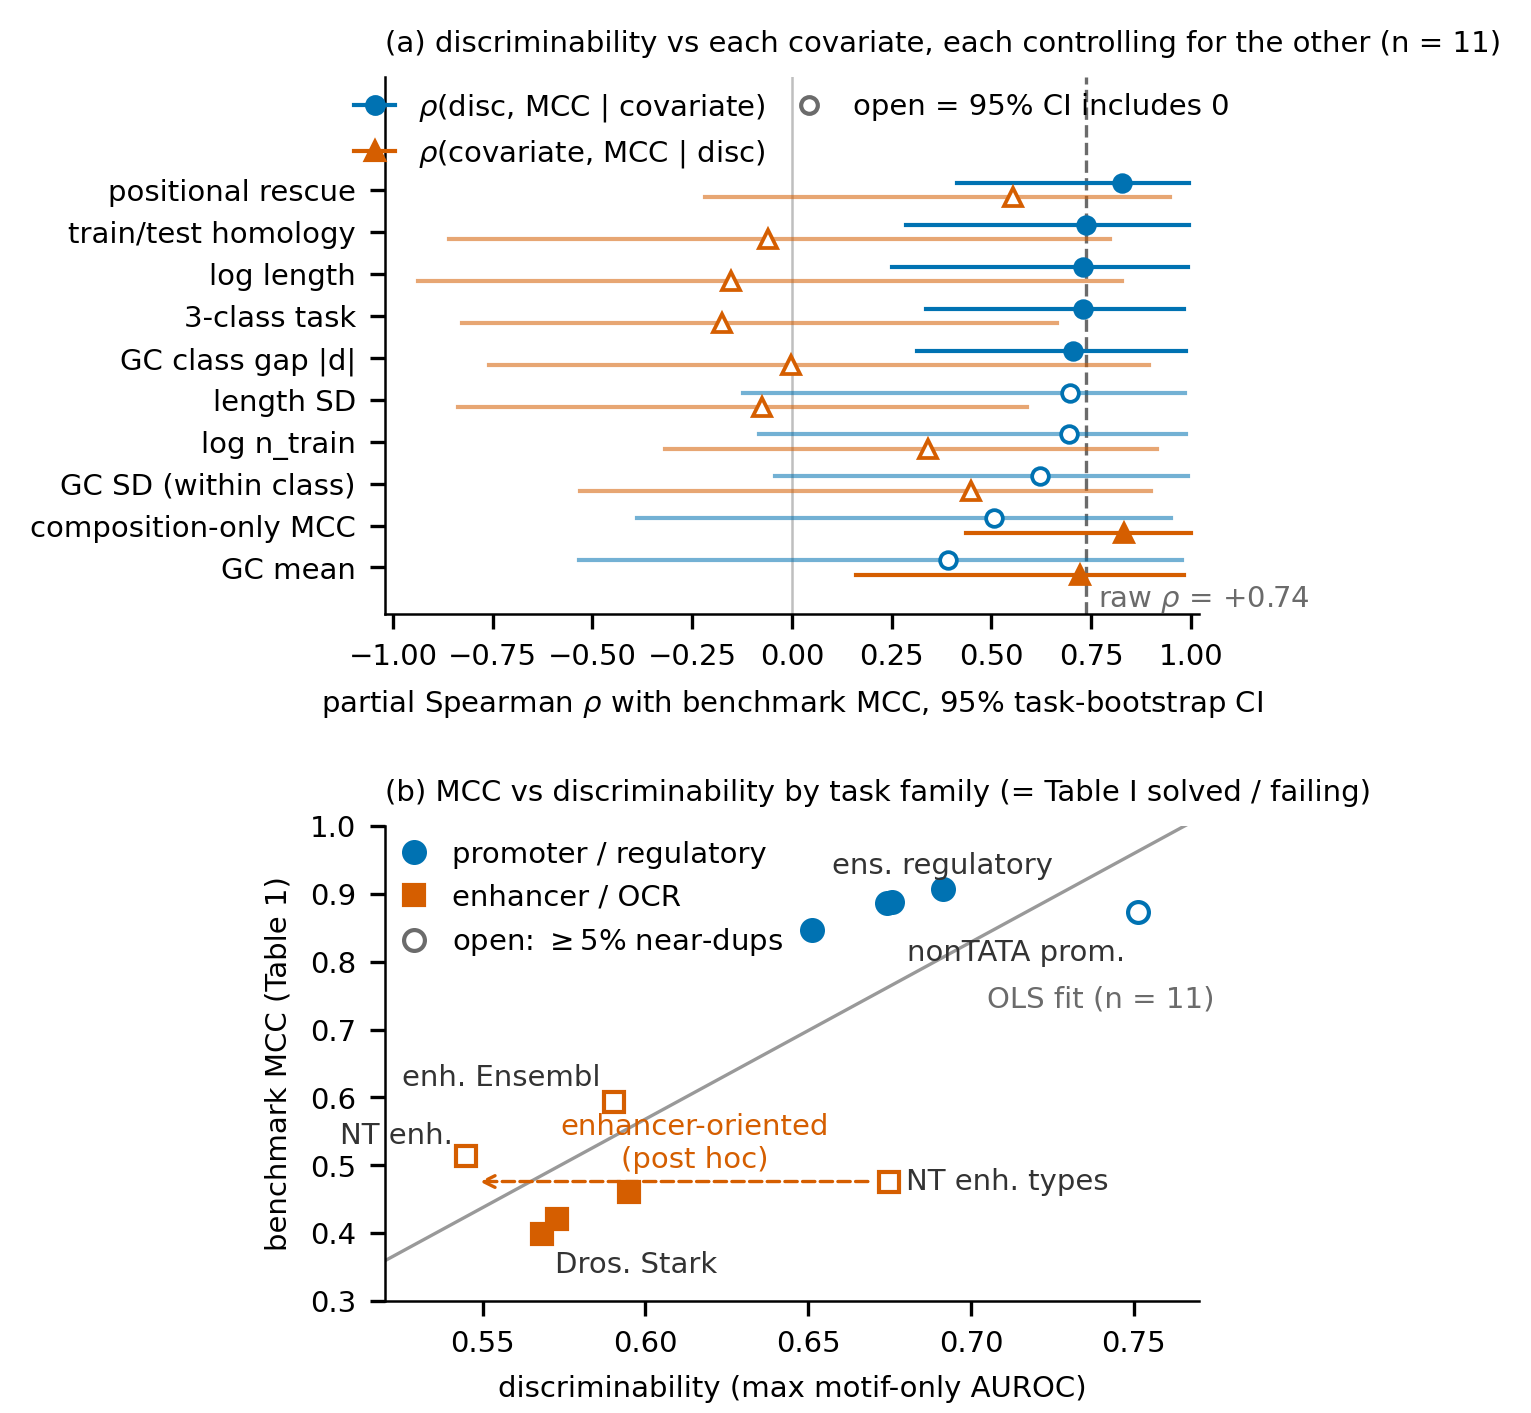
\includegraphics[width=0.6\linewidth]{figs/multivar_covariates_cropped.png}
\caption{Route~1 covariates on the 11 TF-motif tasks. (a) Partial Spearman correlation of benchmark
MCC with discriminability given each covariate (circles) and with the covariate given
discriminability (triangles); 95\% task-bootstrap CIs; open symbols: CI includes 0. (b) Benchmark
MCC vs.\ discriminability by task family (= Table~I's solved/failing split; ``OCR'': open-chromatin);
open symbols: tasks with $\ge$5\% train/test near-duplicates by 8-mer Jaccard $\ge$0.7; arrow: the
post hoc enhancer-oriented discriminability of \task{nt\_enhancers\_types}. The 11 tasks are
\smNdistinct\ distinct sequence sets (Table~\ref{tab:subsets}).
Source: \src{results/upgrades/figures/multivar\_covariates.png} (in-figure footnote cropped).}
\label{fig:multivar}
\end{figure}

% =====================================================================
\section{Provenance of the negatives}\label{sec:s3}

The paper traces the Route-3 composition gap mainly to GC-rich positives, with genomic negatives
drawn from gene-distal or unmarked DNA. This section gives the evidence
(Tables~\ref{tab:provcompact}--\ref{tab:provrules}).

\subsection{Where the negatives come from}
\task{cohn} negatives are random 500-bp windows at least 15\,kb from genes and outside liver H3K27ac
peaks~\cite{cohn2018}. On GRCh38, \smCohnPc\ \smCohnPcCI\ of them lie at least 15\,kb from every
GENCODE v44 protein-coding gene, against \smRandPc\ of random windows. They are gene-distal but not
gene-free: only \smCohnAll\ lie at least 15\,kb from every GENCODE gene of any biotype, \smCohnInGene\
lie inside a gene (\smCohnIntron\ in introns, mostly of non-coding genes; \smCohnExon\ in exons),
\smCohnSthirteen\ are ChromHMM state~13 in all nine lines, and \smCohnEnhAny\ carry an enhancer state in
at least one line.

Genomic \task{nt\_enhancers} training negatives (iEnhancer-2L~\cite{liu2016}) are ChromHMM low-signal
state~13 (a nine-mark model without H3K9me3) in all nine ENCODE
lines~\cite{ernst2011}: \smStrainNeg, against \smSrand\ of random windows. This rule also reproduces
the published candidate count (\smRuleCount\ 200-bp fragments against \smRulePub;
Table~\ref{tab:provrules}). The test negatives (iEnhancer-EL~\cite{liu2018}) differ: only
\smStestNeg\ \smStestNegCI\ are state~13 in all nine lines, and their FASTA headers point to single
state-13 segments rather than to the nine-line intersection (the construction is inferred post hoc
from the headers). They are equally AT-rich (Table~\ref{tab:provsplit}). Most of the training data are not genomic: \smSynTrNeg\ of the
training negatives (\smSynTrNegN) and \smSynTrPos\ of the training positives are RankGAN-synthetic
sequences~\cite{geng2022} with no locus, and only \smGenomicAll\ of all \task{nt\_enhancers} sequences
(\smGenomicAllN, including the whole test split) are genomic.

Such DNA lies in AT-rich isochores~\cite{costantini2006}: \smCohnIso\ of \task{cohn} negatives and
\smNtIso\ of genomic \task{nt\_enhancers} negatives are in L1+L2 isochores (100-kb GC below 41\%),
against \smRandIso\ and \smNtRandIso\ of random windows.

TATA-box rates in this section use every sequence: positives against negatives, \smTataAllCohn\ for
\task{cohn} and \smTataAllNt\ for the whole \task{nt\_enhancers} class. The TATA gate and the
motif-only scans (Section~\ref{sec:s4ctl}) use a seeded sample of \smTataSampleN\ sequences per class,
which gives \smTataSubCohn\ and \smTataSubNt.

% generated by bibm/supplement/make_sm_tables.py -- do not edit; sources: neg_provenance_compact_table.csv
\begin{table}[!htbp]
\caption{Provenance of the negatives: composition and genomic context of positives, negatives and rule-drawn or random genomic backgrounds. Source: \src{neg\_provenance\_compact\_table.csv}.}
\label{tab:provcompact}
\centering
\footnotesize
\setlength{\tabcolsep}{3.5pt}
\begin{tabular}{>{\raggedright\arraybackslash}p{0.27\linewidth}rrrrrrrr}
\toprule
Group & $n$ & GC & TATA & L1+L2 & $\ge$15\,kb pc & cCRE & S13 all 9 & enh.\ $\ge$1 \\
\midrule
cohn: positives (H3K27ac peaks) & 13{,}895 & 0.468 & 0.352 & 0.299 & 0.240 & 0.940 & 0.032 & 0.792 \\
cohn: negatives & 13{,}896 & 0.393 & 0.574 & 0.711 & 0.947 & 0.388 & 0.575 & 0.143 \\
cohn: rule, $\ge$15 kb from protein-coding genes (post hoc) & 10{,}000 & 0.393 & 0.581 & 0.720 & 1.000 & 0.346 & 0.580 & 0.137 \\
cohn: rule, $\ge$15 kb from any GENCODE gene (pre-specified) & 10{,}000 & 0.387 & 0.608 & 0.792 & 1.000 & 0.320 & 0.649 & 0.116 \\
cohn: random genome & 10{,}000 & 0.408 & 0.541 & 0.602 & 0.462 & 0.451 & 0.368 & 0.217 \\
nt: positives (genomic, train+test) & 1{,}584 & 0.489 & 0.119 & 0.232 & 0.226 & 0.814 & 0.000 & 0.999 \\
nt: negatives (genomic, train+test) & 1{,}684 & 0.374 & 0.356 & 0.840 & 0.685 & 0.189 & 0.955 & 0.015 \\
nt: negatives, train (iEnhancer-2L benchmark) & 1{,}484 & 0.375 & 0.357 & 0.846 & 0.695 & 0.187 & 0.998 & 0.000 \\
nt: negatives, test (iEnhancer-EL independent set) & 200 & 0.372 & 0.345 & 0.794 & 0.610 & 0.205 & 0.640 & 0.125 \\
nt: negatives (RankGAN-synthetic, train only) & 5{,}889 & 0.406 & 0.296 & n/a & n/a & n/a & n/a & n/a \\
nt: rule, ChromHMM state 13 in all 9 lines (pre-specified secondary) & 10{,}000 & 0.375 & 0.356 & 0.852 & 0.695 & 0.175 & 0.999 & 0.000 \\
nt: rule, non-enhancer (not 4-7) in all 9 lines (pre-specified primary) & 10{,}000 & 0.400 & 0.301 & 0.650 & 0.492 & 0.256 & 0.480 & 0.000 \\
nt: random genome & 10{,}000 & 0.410 & 0.285 & 0.599 & 0.462 & 0.338 & 0.370 & 0.214 \\
\bottomrule
\end{tabular}
\par\smallskip
\begin{minipage}{\linewidth}\footnotesize\raggedright
Point estimates; the 95\% bootstrap CIs (window = resampling unit) are in the source file. GC: local window GC; TATA: fraction with a TBP hit $\ge$1.3 bits/pos; L1+L2: 100-kb GC $<$41\%; $\ge$15\,kb pc: distance $\ge$15\,kb from every GENCODE v44 protein-coding gene; cCRE: any ENCODE V4 cCRE overlap; S13 all 9: ChromHMM low-signal state 13 (a nine-mark model without H3K9me3) in all nine ENCODE lines; enh.\ $\ge$1: an enhancer state in at least one line. `Rule' rows are backgrounds re-drawn by the documented sampling rules; which rule variant is pre-specified and which was added post hoc is stated in each row. RankGAN-synthetic sequences have no locus (n/a). TATA-box rates here use every sequence of each group. The TATA gate and the motif-only scans (Table~\ref{tab:ctlmotif}) use a seeded sample of 4{,}000 sequences per class, which gives 34.6\% vs.\ 57.3\% (+22.7 points) for \task{cohn} positives vs.\ negatives and 10.6\% vs.\ 31.5\% (+20.9) for the whole \task{nt\_enhancers} class; on all sequences the excess is +22.2 and +20.8 points (\task{nt\_enhancers} whole class: 10.2\% vs.\ 31.0\%; Table~\ref{tab:provd1}).
\end{minipage}
\end{table}


\subsection{Why the negatives are AT-rich, and why that is not the whole gap}
Relative to random genome, the sampling rules shift the negatives toward AT (TATA-box rate
\smTataShiftCohn\ and \smTataShiftNt\ points for \task{cohn} and genomic \task{nt\_enhancers}). That
shift is a minority of the positive--negative gap (Table~\ref{tab:provd1}). The negative side carries
\smShareCohnGC\ \smShareCohnGCCI\ (\task{cohn}) and \smShareNtGC\ \smShareNtGCCI\ (genomic
\task{nt\_enhancers}) of the GC gap, and only \smShareWholeGC\ over the whole, mostly synthetic
\task{nt\_enhancers} class; of the TATA gap it carries \smShareCohnTata\ and \smShareNtTata\
(\smShareWholeTata\ over the whole class). The rest (\smPosShareCohnGC\ and \smPosShareNtGC\ of the GC
gap; \smPosShareWholeGC\ over the whole class) is the positives' GC-richness and TATA depletion
relative to random genome.

Backgrounds re-drawn by the documented rules, with unstated details inferred post hoc, reproduce the
negatives' GC. For \task{cohn}, a rule restricted to protein-coding genes differs from the negatives
by \smBgPcGC\ in GC and \smBgPcTata\ in TATA-box rate (six pooled background draws); for
\task{nt\_enhancers}, the state-13 rule differs by \smBgSthirteenGC\ and \smBgSthirteenTata. The
pre-specified rule variants fare worse: the all-gene \task{cohn} rule over-shoots the negatives' AT
shift, and the literal \task{nt\_enhancers} rule (non-enhancer states in all nine lines) does not
explain it (Table~\ref{tab:provd1}).

% generated by bibm/supplement/make_sm_tables.py -- do not edit; sources: neg_provenance_tests.csv, neg_provenance_nt_wholeclass.csv
\begin{table}[!htbp]
\caption{How much of the positive--negative composition gap the negatives' sampling explains (decision rule D1). Source: \src{neg\_provenance\_tests.csv},\enspace \src{neg\_provenance\_nt\_wholeclass.csv}.}
\label{tab:provd1}
\centering
\scriptsize
\setlength{\tabcolsep}{3pt}
\begin{tabular}{llrrlll}
\toprule
Data & Metric & POS$-$NEG & Random$-$NEG & Neg.-side share [CI] & $f_\mathrm{rule}$ [CI] & D1 verdict \\
\midrule
\task{cohn} & GC (window) & +0.075 & +0.015 & 20\% [18, 23] & 1.36 [1.22, 1.54] & explained \\
\task{cohn} & TATA-box rate & −0.222 & −0.033 & 15\% [9, 20] & 2.05 [1.54, 3.18] & explained \\
\task{cohn} & GC (100 kb) & +0.051 & +0.016 & 31\% [28, 33] & 1.38 [1.30, 1.46] & explained \\
\task{cohn} & L1+L2 isochore & −0.412 & −0.109 & 26\% [24, 29] & 1.75 [1.61, 1.92] & explained \\
genomic \task{nt\_enh.} & GC (window) & +0.115 & +0.036 & 31\% [28, 34] & 0.28 [0.21, 0.35] & not explained \\
genomic \task{nt\_enh.} & TATA-box rate & −0.236 & −0.070 & 30\% [21, 37] & 0.23 [0.05, 0.43] & not explained \\
genomic \task{nt\_enh.} & GC (100 kb) & +0.079 & +0.028 & 36\% [34, 38] & 0.23 [0.18, 0.27] & not explained \\
genomic \task{nt\_enh.} & L1+L2 isochore & −0.608 & −0.241 & 40\% [37, 42] & 0.21 [0.16, 0.26] & not explained \\
whole \task{nt\_enh.} class$^\ast$ & GC (window) & +0.083 & +0.011 & 13.5\% [11, 16] & -- & -- \\
whole \task{nt\_enh.} class$^\ast$ & TATA-box rate & −0.208 & −0.024 & 11.8\% [5, 17] & -- & -- \\
\bottomrule
\end{tabular}
\par\smallskip
\begin{minipage}{\linewidth}\footnotesize\raggedright
$^\ast$ post hoc; mostly RankGAN-synthetic sequences. The gap POS$-$NEG splits into (POS$-$random genome) $+$ (random genome$-$NEG); the negative-side share is the second term's share: the part of the gap that comes from where the negatives were sampled. The rest is the positives' departure from random genome (their GC-richness and TATA depletion). $f_\mathrm{rule}$ = (random$-$rule background)/(random$-$NEG) for the pre-specified rule backgrounds (\task{cohn}: $\ge$15\,kb from any GENCODE gene; \task{nt\_enhancers}: literal non-enhancer states in all nine lines); $f_\mathrm{rule}{>}1$ means the rule background over-shoots the negatives' AT shift. The verdict answers only whether that documented rule reproduces the negatives' shift from random genome. All sequences are used (for the seeded 4,000-per-class sample of the motif scan, see the note to Table~\ref{tab:provcompact}).
\end{minipage}
\end{table}


\subsection{Chromosomes}
The chromosome distribution of the genomic \task{nt\_enhancers} negatives is consistent with the
state-13 rule (\smChromNtChi; homogeneity test against the rule background). That of the \task{cohn}
negatives is not reproduced by any rule background (\smChromCohnP): there are \smChrNineNeg\ chr9
negatives against \smChrNinePos\ chr9 positives (\smChrNineExp\ expected under the rule background).
This skew is unexplained and is a potential chromosome-level label shortcut.

% generated by bibm/supplement/make_sm_tables.py -- do not edit; sources: neg_provenance_nt_by_split.csv, neg_provenance_nt_origin.csv
\begin{table}[!htbp]
\caption{Genomic \task{nt\_enhancers} negatives by split: training (iEnhancer-2L) vs.\ test (iEnhancer-EL independent set). Source: \src{neg\_provenance\_nt\_by\_split.csv},\enspace \src{neg\_provenance\_nt\_origin.csv}.}
\label{tab:provsplit}
\centering
\footnotesize
\begin{tabular}{lllr}
\toprule
Metric & Train negatives ($n{=}1{,}484$) [CI] & Test negatives ($n{=}200$) [CI] & Train positives \\
\midrule
ChromHMM state 13 in all 9 lines & 0.998 [0.995, 1.000] & 0.640 [0.570, 0.700] & 0.000 \\
enhancer state in $\ge$1 line & 0.000 [0.000, 0.000] & 0.125 [0.080, 0.170] & 0.999 \\
GC (window) & 0.375 [0.371, 0.378] & 0.372 [0.360, 0.383] & 0.491 \\
TATA-box rate & 0.357 [0.334, 0.382] & 0.345 [0.275, 0.405] & 0.119 \\
L1+L2 isochore & 0.846 [0.829, 0.864] & 0.794 [0.734, 0.849] & 0.222 \\
any cCRE overlap & 0.187 [0.168, 0.207] & 0.205 [0.150, 0.260] & 0.821 \\
\bottomrule
\end{tabular}
\par\smallskip
\begin{minipage}{\linewidth}\footnotesize\raggedright
Synthetic share (RankGAN; no locus): 5{,}889 of 7{,}484 training negatives (78.7\%), 5{,}146 of 7{,}484 training positives (68.8\%); 76.6\% of all 7{,}684 negatives and 71.8\% of all 15{,}368 sequences; no test sequence is synthetic. The test negatives' FASTA headers point to single ChromHMM state-13 segments rather than to the nine-line intersection (inferred post hoc from the headers).
\end{minipage}
\end{table}

% generated by bibm/supplement/make_sm_tables.py -- do not edit; sources: neg_provenance_chromhmm_rule_counts.csv
\begin{table}[!htbp]
\caption{Which ChromHMM definition reproduces the published iEnhancer-2L candidate counts (post hoc). Source: \src{neg\_provenance\_chromhmm\_rule\_counts.csv}.}
\label{tab:provrules}
\centering
\footnotesize
\begin{tabular}{lrrr}
\toprule
Rule (hg19 ChromHMM, nine ENCODE lines) & 200-bp fragments & Published count & Ratio \\
\midrule
state13\_all9 (low signal in all nine) & 5{,}260{,}191 & 5{,}257{,}994 & 1.0004 \\
nonenhancer\_all9 (not states 4-7 in all nine) & 11{,}148{,}205 & 5{,}257{,}994 & 2.1202 \\
nonenh\_nonprom\_all9 (not states 1-7 in all nine) & 10{,}933{,}257 & 5{,}257{,}994 & 2.0794 \\
state13or12\_all9 (low signal or Repressed in all nine) & 6{,}302{,}797 & 5{,}257{,}994 & 1.1987 \\
state13to15\_all9 (low signal or Repetitive/CNV in all nine) & 5{,}287{,}100 & 5{,}257{,}994 & 1.0055 \\
strongenh\_all9 (states 4-5 in all nine) & 742 & 742 & 1.0000 \\
enhancer\_all9 (states 4-7 in all nine) & 4{,}222 & 742 & 5.6900 \\
weakenh\_any (states 6-7 in >=1 of nine) & 2{,}460{,}484 & 370{,}517 & 6.6407 \\
enhancer\_any (states 4-7 in >=1 of nine) & 3{,}004{,}738 & 370{,}517 & 8.1096 \\
enhancer\_any\_not\_strong\_all9 (4-7 in >=1, not 4-5 in all nine) & 3{,}003{,}996 & 370{,}517 & 8.1076 \\
\bottomrule
\end{tabular}
\par\smallskip
\begin{minipage}{\linewidth}\footnotesize\raggedright
Published counts: non-enhancer candidates for the non-enhancer rules, 742 strong enhancers for the strong rule, weak-enhancer candidates for the weak rules. `State 13 in all nine' reproduces the non-enhancer count; it does not separate state 13 from states 13--15, and no reading reproduces the weak count.
\end{minipage}
\end{table}


\subsection{What the provenance shows and does not show}\label{sec:s3wider}
The coordinate analysis in the paper refutes core-promoter leakage for \task{cohn} (TATA-flagged
negatives are depleted at TSSs; Fisher $p$~=~\smCohnTssP); on the genomic \task{nt\_enhancers} subset
(\smNtMapped\ of its sequences) the depletion is directional but underpowered ($p=\smNtTssP$). The
provenance shows that most
of the composition gap is the positives' own GC-richness, with the negative-sampling choices
(gene-distal windows; ChromHMM low-signal chromatin) contributing the rest. Neither is a data error,
and neither separates artifactual from biological composition. Route~3's critique is one of benchmark
design: on these otherwise hard tasks composition alone supplies most of the separability
(composition-only AUROC \smCompZero\ and \smCompZeroNt\ against $k$-mer \smAzero\ and \smAzeroNt\ for
\task{cohn} and \task{nt\_enhancers}), whatever the composition's origin.

% =====================================================================
\section{Route-3 matching sensitivity and the control-motif panel}\label{sec:s4}

\subsection{Designs and the pre-specified rule}
Composition equalization resamples the negatives, within each split, to the positives' histogram of
a propensity score fit on the 20-dimensional mono- plus dinucleotide signature~\cite{rosenbaum1983}.
In this section \emph{matching} means this equalization (the paper's composition-equalized intervention), and
its kept negatives are the \emph{matched} negatives; it is not the GC-matched test subset of the frozen
probes (Section~\ref{sec:s5}). The equalizer is \emph{one-sided}: it removes negatives only.
The released equalizer ($\alpha{=}1$) keeps \smKeptCohn\ of \task{cohn} negatives (max$|$SMD$|$ \smSMDpub\ on
the released equalized split; \smSMDredraw\ on the seed-42 re-draw). We compare it with size-matched random
negatives (\smNrandom\ draws per level) in designs that differ in what they hold fixed
(Table~\ref{tab:psmdesigns}):
\begin{itemize}
\item \emph{within} (retrained on matched vs.\ random negatives, each scored on its own reduced test;
unpaired). The pre-specified decision rule uses this design at strictness $\alpha=1$
(Table~\ref{tab:psmdecision});
\item \emph{undistorted test} (retrained on matched or random negatives, both scored on the untouched
original test; paired);
\item \emph{model fixed} (the original model scored on the matched vs.\ random test subsets; paired);
\item removal-free overlap weighting~\cite{li2018}, retrained or with the original model, against a
permuted-weight placebo;
\item positive-side matching (positives subsampled to the negatives' propensity histogram; every
negative kept);
\item two-sided 1:1 caliper matching (both classes subsampled; the test stays balanced).
\end{itemize}

% generated by bibm/supplement/make_sm_tables.py -- do not edit; sources: psm_sensitivity_decision.csv
\begin{table}[!htbp]
\caption{Decision table for composition matching at the released equalizer's retention ($\alpha{=}1$; $k$-mer AUROC; retrained within-arm design). The rule and the \task{cohn}, original \task{nt\_enhancers} and control rows are pre-specified; the two leak-free \task{nt\_enhancers} rows apply the same rule post hoc. Source: \src{psm\_sensitivity\_decision.csv}.}
\label{tab:psmdecision}
\centering
\scriptsize
\setlength{\tabcolsep}{2pt}
\begin{tabular}{>{\raggedright\arraybackslash}p{0.11\linewidth}lllllrrr>{\raggedright\arraybackslash}p{0.055\linewidth}>{\raggedright\arraybackslash}p{0.085\linewidth}}
\toprule
Data & Original [CI] & Random (10 draws) & Matched, seed 42 [CI] & Seeds 42--44 & Released & Kept & Test neg. & max$|$SMD$|$ & Failed & Verdict \\
\midrule
\task{cohn} & 0.805 [0.795, 0.814] & 0.765 (0.738--0.793) & 0.621 [0.582, 0.658] & 0.613--0.637 & 0.613 & 4.5\% & 228 & 0.07 & (i-a) & supported, with a size component \\
\task{nt\_enhancers}, original test & 0.850 [0.812, 0.889] & 0.807 (0.763--0.832) & 0.799 [0.722, 0.871] & 0.707--0.799 & 0.748 & 4.9\% & 36 & 0.30 & (i-a), (i-b) & not supported \\
\task{nt\_enhancers}, leak-free test$^\dagger$ & 0.735 [0.670, 0.790] & 0.723 (0.689--0.751) & 0.684 [0.587, 0.782] & 0.575--0.684 & 0.628 & 4.9\% & 36 & 0.30 & (i-b) & not supported \\
\task{nt\_enhancers}, leak-free refit$^\dagger$ & 0.804 [0.760, 0.844] & 0.786 (0.743--0.818) & 0.706 [0.623, 0.788] & 0.563--0.706 & 0.624 & 4.9\% & 36 & 0.31 & (i-b) & not supported \\
GC-balanced control & 0.763 [0.743, 0.786] & 0.754 (0.729--0.775) & 0.674 [0.632, 0.719] & 0.650--0.674 & 0.661 & 42.9\% & 217 & 0.06 & none & supported \\
\bottomrule
\end{tabular}
\par\smallskip
\begin{minipage}{\linewidth}\footnotesize\raggedright
Released: AUROC on the released equalized split. Random: mean (range) over 10 size-matched random negative draws; matched: the released equalizer rule re-drawn with selection seed 42 (the verdict uses seed 42, as pre-specified). Criteria: (i-a) size effect $\le$ tolerance $\tau=\max(0.03$, half-width of the original CI); (i-b) matched below every random seed and its upper CI below the random mean; (ii-a) overlap-weighted AUROC below every permuted-weight placebo, upper CI below the placebo mean, and a drop $\ge$0.5$\times$ the matching drop; (ii-b) the same for two-sided 1:1 matching at caliper 0.2 SD. SUPPORTED: all four; SUPPORTED-WITH-SIZE-COMPONENT: all but (i-a); NOT SUPPORTED: (i-b) fails or both (ii) fail. max$|$SMD$|$ of the re-drawn matched set; the released equalized \task{cohn} split has 0.06. 100 of the 400 \task{nt\_enhancers} test sequences, all of them positives, occur verbatim in the training split. $^\dagger$Post hoc: the leak-free rows remove them from every test set (leak-free test; same models) or refit every arm without their training copies and score the full test set (leak-free refit). The verdict is the same in all three \task{nt\_enhancers} rows.
\end{minipage}
\end{table}


\subsection{\texorpdfstring{\task{cohn}}{cohn}: shortcut removal or sample loss?}
Random reduction to \smKeptCohn\ of the negatives lowers $k$-mer AUROC from \smAzero\ to \smAr\ (range
\smArRange), and composition matching to \smAm\ \smAmCI\ in one matching draw (selection seed 42;
seeds 42--44 give \smAmSeeds; the released equalized split \smPub). The total drop of \smDropTotal\ splits into
a size effect of \smSizeEff\ (\smSizeShare\ \smSizeShareCI\ of the drop) and a matched-vs-random effect
of \smMvr\ (\smMvrShare\ \smMvrShareCI; Table~\ref{tab:psmdecomp}). The size share depends on the
matching draw: over \smDraws\ equally valid draws of the released equalizer the matched AUROC spans
\smDrawRange\ (median \smDrawMedian), which puts the size share at about \smSizeShareMedian\ at the
median draw (\smSizeShareMedianExact) and \smSizeShareMax\ at the highest draw; the mean of selection
seeds 42--44 gives \smSizeShareSeeds. Because the size effect exceeds the pre-specified tolerance
(\smTau), the verdict is ``supported, with a size component''.

\emph{Test distortion and negative removal.} With the test held fixed, a model trained on matched
negatives scores \smTrainOnly\ on the untouched original test, against \smTrainOnlyR\ for one trained on
random negatives (difference \smTrainOnlyD). With the model held fixed, the original model scores
\smFixed\ on the matched test subset and \smFixedR\ on random subsets (\smFixedD). Changing only the
test's class ratio moves AUROC by \smRatioOnly, as expected for a prevalence-invariant metric. With no
negative removed at all, matching the positives to the negatives (\smFfourPos\ of positives kept,
every negative kept) gives \smFfour\ \smFfourCI\ against \smFfourR\ for random positive subsets. Under
removal-free overlap weighting the original model scores \smOverlapFixed\ against a placebo of
\smOverlapPlacebo, and two-sided 1:1 matching at caliper 0.2\,SD gives \smOneToOne\ against \smOneToOneR.

\emph{Sweeps.} Along the strictness sweep (Table~\ref{tab:psmsweep}; Fig.~\ref{fig:psm}) the gap
between random and matched negatives grows with balance, from \smSweepGapLoose\ at \smSweepKeptLoose\
of negatives kept to \smSweepGapHalf\ at \smSweepKeptHalf\ and \smSweepGapNine\ at \smSweepKeptNine,
then levels off (\smSweepGapOne\ at $\alpha{=}1$; this last step lies within the
matching-draw variation above). Meanwhile the size-matched random controls fall from
\smSweepRandLoose\ to \smSweepRandOne: that fall is the size component. Along the caliper sweep
(Table~\ref{tab:psmcaliper}; Fig.~\ref{fig:psmcal}) random 1:1 subsets stay at \smCalRandRange, while
the matched gap rises from \smCalGapTwo\ at a caliper of 2\,SD to \smCalGapPtTwo\ at 0.2\,SD, where both
classes are balanced.

% generated by bibm/supplement/make_sm_tables.py -- do not edit; sources: psm_sensitivity_decision.csv
\begin{table}[!htbp]
\caption{Designs at $\alpha{=}1$ that change what matching can distort: which test set is scored, whether the model is retrained, and whether any negative is removed ($k$-mer AUROC; composition-balanced: matched with selection seed 42, or overlap-weighted; random / placebo: mean of 10 size-matched random draws, or of the permuted-weight placebo for the weighting rows). Source: \src{psm\_sensitivity\_decision.csv}.}
\label{tab:psmdesigns}
\centering
\scriptsize
\setlength{\tabcolsep}{3pt}
\begin{tabular}{>{\raggedright\arraybackslash}p{0.46\linewidth}>{\raggedright\arraybackslash}p{0.17\linewidth}rrr}
\toprule
Design & Pairing & Composition-balanced & Random / placebo & Difference \\
\midrule
\multicolumn{5}{@{}l}{\emph{\task{cohn}}} \\
Retrained on matched vs.\ random negatives, each scored on its own reduced test & unpaired (within) & 0.621 & 0.765 & +0.144 \\
Retrained on matched vs.\ random negatives, scored on the untouched original test & paired (undistorted test) & 0.584 & 0.765 & +0.181 \\
Original model scored on the matched vs.\ random test subsets & paired (model fixed) & 0.595 & 0.803 & +0.209 \\
Original model on the original test, class ratio changed only & size/ratio check & -- & -- & +0.001 \\
Original model, overlap-weighted original test vs.\ permuted-weight placebo & removal-free, paired & 0.609 & 0.806 & +0.197 \\
Retrained with overlap weights vs.\ placebo & removal-free & 0.671 & 0.805 & +0.134 \\
Positives matched to the negatives, every negative kept, vs.\ random positive subsets & no negative removed & 0.622 & 0.780 & +0.157 \\
Two-sided 1:1 caliper 0.2 SD vs.\ random 1:1 & balanced test & 0.688 & 0.802 & +0.114 \\
\multicolumn{5}{@{}l}{\emph{\task{nt\_enhancers}, leak-free test}} \\
Retrained on matched vs.\ random negatives, each scored on its own reduced test & unpaired (within) & 0.684 & 0.723 & +0.039 \\
Retrained on matched vs.\ random negatives, scored on the untouched original test & paired (undistorted test) & 0.570 & 0.715 & +0.145 \\
Original model scored on the matched vs.\ random test subsets & paired (model fixed) & 0.535 & 0.735 & +0.200 \\
Original model on the original test, class ratio changed only & size/ratio check & -- & -- & −0.001 \\
Original model, overlap-weighted original test vs.\ permuted-weight placebo & removal-free, paired & 0.311$^\ddagger$ & 0.738 & +0.427 \\
Retrained with overlap weights vs.\ placebo & removal-free & 0.406$^\ddagger$ & 0.736 & +0.330 \\
Positives matched to the negatives, every negative kept, vs.\ random positive subsets & no negative removed$^\S$ & 0.464 & 0.746 & +0.282 \\
Two-sided 1:1 caliper 0.2 SD vs.\ random 1:1 & balanced test & 0.594 & 0.729 & +0.135 \\
\multicolumn{5}{@{}l}{\emph{GC-balanced control}} \\
Retrained on matched vs.\ random negatives, each scored on its own reduced test & unpaired (within) & 0.674 & 0.754 & +0.081 \\
Retrained on matched vs.\ random negatives, scored on the untouched original test & paired (undistorted test) & 0.703 & 0.754 & +0.051 \\
Original model scored on the matched vs.\ random test subsets & paired (model fixed) & 0.690 & 0.762 & +0.072 \\
Original model on the original test, class ratio changed only & size/ratio check & -- & -- & +0.001 \\
Original model, overlap-weighted original test vs.\ permuted-weight placebo & removal-free, paired & 0.687 & 0.763 & +0.076 \\
Retrained with overlap weights vs.\ placebo & removal-free & 0.695 & 0.762 & +0.067 \\
Positives matched to the negatives, every negative kept, vs.\ random positive subsets & no negative removed & 0.662 & 0.727 & +0.065 \\
Two-sided 1:1 caliper 0.2 SD vs.\ random 1:1 & balanced test & 0.683 & 0.755 & +0.072 \\
\bottomrule
\end{tabular}
\par\smallskip
\begin{minipage}{\linewidth}\footnotesize\raggedright
`Paired' designs hold either the model or the test set fixed, so a difference cannot come from a changed test distribution (undistorted test) or from retraining on fewer negatives (model fixed). $^\ddagger$ the overlap weights over-correct (the composition-only model's weighted AUROC falls below 0.5), so only the direction is interpretable. $^\S$ underpowered (17 test positives). Differences are computed from unrounded values; CIs of the within, undistorted-test and model-fixed contrasts are in Table~\ref{tab:psmdecomp}.
\end{minipage}
\end{table}

% generated by bibm/supplement/make_sm_tables.py -- do not edit; sources: psm_sensitivity_decomposition_ci.csv
\begin{table}[!htbp]
\caption{Decomposition of the matching drop at $\alpha{=}1$, with two-level paired bootstrap CIs (post hoc P7): size effect (original $-$ random) and matched-vs-random effect (random $-$ matched). Source: \src{psm\_sensitivity\_decomposition\_ci.csv}.}
\label{tab:psmdecomp}
\centering
\scriptsize
\setlength{\tabcolsep}{3pt}
\begin{tabular}{llllr}
\toprule
Design & Model & Size effect [CI] & Matched-vs-random [CI] & Test neg.\ scored \\
\midrule
\multicolumn{5}{@{}l}{\emph{\task{cohn}}} \\
within (retrained, own test) & $k$-mer & +0.040 [+0.022, +0.059] & +0.144 [+0.102, +0.184] & 228 \\
within (retrained, own test) & composition-only & +0.046 [+0.030, +0.064] & +0.184 [+0.138, +0.223] & 228 \\
within (retrained, own test), seeds 42--44 & $k$-mer & +0.040 [+0.022, +0.059] & +0.141 [+0.107, +0.177] & 228 \\
within (retrained, own test), seeds 42--44 & composition-only & +0.046 [+0.030, +0.064] & +0.173 [+0.133, +0.205] & 228 \\
undistorted test (retrained, original test) & $k$-mer & +0.040 [+0.034, +0.046] & +0.181 [+0.166, +0.195] & 3{,}474 \\
undistorted test (retrained, original test) & composition-only & +0.046 [+0.039, +0.053] & +0.216 [+0.199, +0.233] & 3{,}474 \\
model fixed (original model) & $k$-mer & -- & +0.209 [+0.169, +0.249] & 228 \\
model fixed (original model) & composition-only & -- & +0.229 [+0.187, +0.270] & 228 \\
\multicolumn{5}{@{}l}{\emph{\task{nt\_enhancers}, leak-free test}} \\
within (retrained, own test) & $k$-mer & +0.011 [−0.029, +0.052] & +0.039 [−0.077, +0.145] & 36 \\
within (retrained, own test) & composition-only & +0.018 [−0.022, +0.058] & +0.134 [−0.008, +0.273] & 36 \\
within (retrained, own test), seeds 42--44 & $k$-mer & +0.011 [−0.029, +0.052] & +0.091 [−0.029, +0.217] & 36 \\
within (retrained, own test), seeds 42--44 & composition-only & +0.018 [−0.022, +0.058] & +0.106 [−0.036, +0.246] & 36 \\
undistorted test (retrained, original test) & $k$-mer & +0.020 [−0.004, +0.042] & +0.145 [+0.055, +0.235] & 200 \\
undistorted test (retrained, original test) & composition-only & +0.028 [+0.006, +0.051] & +0.265 [+0.154, +0.356] & 200 \\
model fixed (original model) & $k$-mer & -- & +0.200 [+0.117, +0.294] & 36 \\
model fixed (original model) & composition-only & -- & +0.236 [+0.149, +0.329] & 36 \\
\multicolumn{5}{@{}l}{\emph{GC-balanced control}} \\
within (retrained, own test) & $k$-mer & +0.009 [−0.009, +0.028] & +0.081 [+0.040, +0.123] & 217 \\
within (retrained, own test) & composition-only & +0.021 [+0.000, +0.043] & +0.041 [−0.004, +0.090] & 217 \\
within (retrained, own test), seeds 42--44 & $k$-mer & +0.009 [−0.009, +0.028] & +0.091 [+0.058, +0.131] & 217 \\
within (retrained, own test), seeds 42--44 & composition-only & +0.021 [+0.000, +0.043] & +0.080 [+0.031, +0.127] & 217 \\
undistorted test (retrained, original test) & $k$-mer & +0.009 [−0.000, +0.018] & +0.051 [+0.033, +0.070] & 865 \\
undistorted test (retrained, original test) & composition-only & +0.014 [+0.002, +0.028] & +0.098 [+0.075, +0.123] & 865 \\
model fixed (original model) & $k$-mer & -- & +0.072 [+0.039, +0.111] & 217 \\
model fixed (original model) & composition-only & -- & +0.076 [+0.039, +0.116] & 217 \\
\bottomrule
\end{tabular}
\par\smallskip
\begin{minipage}{\linewidth}\footnotesize\raggedright
Bootstrap: test sequences (shared by every arm) $\times$ random seeds, 1000 resamples; the models are fixed, so training-set variability is not resampled. In the model-fixed design the original model is scored on the matched vs.\ random test subsets, so there is no size term. The composition-only rows show how much composition signal the same selection removes; they are the reference for reading the $k$-mer rows. Within-design rows use one matching draw (seed 42) unless marked.
\end{minipage}
\end{table}

% generated by bibm/supplement/make_sm_tables.py -- do not edit; sources: psm_sensitivity_summary.csv
\begin{table}[!htbp]
\caption{Matching-strictness sweep: composition-matched vs.\ size-matched random negatives at every level (retrained, within-arm design; $k$-mer AUROC). Source: \src{psm\_sensitivity\_summary.csv}.}
\label{tab:psmsweep}
\centering
\scriptsize
\setlength{\tabcolsep}{3.5pt}
\begin{tabular}{rrrrlllrr}
\toprule
$\alpha$ & Neg.\ kept & Test neg. & max$|$SMD$|$ & Matched, seed 42 [CI] & Seeds 42--44 & Random (range) & Gap & Comp.-only gap \\
\midrule
\multicolumn{9}{@{}l}{\emph{\task{cohn}}} \\
0.02 & 92.9\% & 3{,}255 & 0.99 & 0.804 [0.794, 0.814] & 0.801--0.804 & 0.806 (0.802--0.808) & +0.001 & +0.004 \\
0.05 & 83.3\% & 2{,}957 & 0.96 & 0.799 [0.789, 0.809] & 0.795--0.799 & 0.805 (0.804--0.809) & +0.007 & +0.010 \\
0.10 & 69.7\% & 2{,}526 & 0.91 & 0.787 [0.776, 0.799] & 0.787--0.793 & 0.803 (0.800--0.808) & +0.016 & +0.017 \\
0.20 & 49.1\% & 1{,}852 & 0.81 & 0.771 [0.757, 0.784] & 0.768--0.771 & 0.801 (0.796--0.807) & +0.029 & +0.038 \\
0.30 & 35.0\% & 1{,}376 & 0.71 & 0.745 [0.728, 0.759] & 0.745--0.764 & 0.798 (0.794--0.808) & +0.053 & +0.059 \\
0.40 & 25.2\% & 1{,}031 & 0.61 & 0.725 [0.707, 0.744] & 0.725--0.745 & 0.797 (0.789--0.809) & +0.071 & +0.086 \\
0.50 & 18.4\% & 781 & 0.51 & 0.712 [0.693, 0.732] & 0.706--0.712 & 0.794 (0.783--0.801) & +0.082 & +0.119 \\
0.60 & 13.6\% & 597 & 0.41 & 0.670 [0.645, 0.693] & 0.670--0.708 & 0.790 (0.773--0.803) & +0.119 & +0.136 \\
0.70 & 10.2\% & 465 & 0.32 & 0.665 [0.639, 0.690] & 0.665--0.687 & 0.787 (0.766--0.800) & +0.122 & +0.168 \\
0.80 & 7.7\% & 364 & 0.24 & 0.648 [0.618, 0.677] & 0.648--0.676 & 0.782 (0.760--0.807) & +0.134 & +0.173 \\
0.90 & 5.8\% & 285 & 0.15 & 0.619 [0.586, 0.653] & 0.619--0.640 & 0.779 (0.759--0.804) & +0.160 & +0.205 \\
1.00 & 4.5\% & 228 & 0.07 & 0.621 [0.582, 0.658] & 0.613--0.637 & 0.765 (0.738--0.793) & +0.144 & +0.184 \\
\multicolumn{9}{@{}l}{\emph{\task{nt\_enhancers}, leak-free test}} \\
0.02 & 90.8\% & 192 & 1.51 & 0.726 [0.663, 0.787] & 0.726--0.740 & 0.730 (0.723--0.740) & +0.004 & +0.010 \\
0.05 & 78.7\% & 178 & 1.47 & 0.721 [0.656, 0.782] & 0.712--0.721 & 0.732 (0.722--0.756) & +0.012 & +0.008 \\
0.10 & 62.4\% & 157 & 1.38 & 0.709 [0.642, 0.777] & 0.704--0.723 & 0.732 (0.714--0.753) & +0.023 & +0.023 \\
0.20 & 40.4\% & 130 & 1.19 & 0.668 [0.597, 0.736] & 0.668--0.690 & 0.732 (0.719--0.747) & +0.064 & +0.053 \\
0.30 & 27.1\% & 104 & 1.00 & 0.670 [0.593, 0.743] & 0.670--0.690 & 0.733 (0.708--0.756) & +0.063 & +0.072 \\
0.40 & 19.0\% & 86 & 0.81 & 0.666 [0.587, 0.745] & 0.666--0.683 & 0.730 (0.703--0.741) & +0.064 & +0.094 \\
0.50 & 13.8\% & 70 & 0.66 & 0.616 [0.527, 0.696] & 0.616--0.659 & 0.731 (0.706--0.756) & +0.116 & +0.107 \\
0.60 & 10.6\% & 62 & 0.51 & 0.614 [0.516, 0.702] & 0.614--0.644 & 0.726 (0.691--0.762) & +0.112 & +0.109 \\
0.70 & 8.4\% & 54 & 0.36 & 0.608 [0.515, 0.700] & 0.608--0.625 & 0.730 (0.686--0.788) & +0.122 & +0.137 \\
0.80 & 6.8\% & 44 & 0.32 & 0.666 [0.567, 0.759] & 0.630--0.672 & 0.722 (0.680--0.755) & +0.055 & +0.173 \\
0.90 & 5.7\% & 41 & 0.32 & 0.670 [0.567, 0.758] & 0.620--0.670 & 0.721 (0.677--0.772) & +0.051 & +0.131 \\
1.00 & 4.9\% & 36 & 0.30 & 0.684 [0.587, 0.782] & 0.575--0.684 & 0.723 (0.689--0.751) & +0.039 & +0.134 \\
\multicolumn{9}{@{}l}{\emph{GC-balanced control}} \\
0.02 & 97.2\% & 823 & 0.26 & 0.756 [0.731, 0.779] & 0.756--0.759 & 0.761 (0.753--0.767) & +0.006 & +0.010 \\
0.05 & 93.9\% & 782 & 0.25 & 0.758 [0.734, 0.779] & 0.746--0.758 & 0.759 (0.751--0.767) & +0.001 & +0.021 \\
0.10 & 88.9\% & 720 & 0.22 & 0.745 [0.719, 0.769] & 0.745--0.750 & 0.762 (0.756--0.771) & +0.017 & +0.023 \\
0.20 & 80.0\% & 615 & 0.20 & 0.735 [0.709, 0.762] & 0.721--0.735 & 0.760 (0.755--0.771) & +0.025 & +0.029 \\
0.30 & 72.5\% & 527 & 0.17 & 0.726 [0.699, 0.754] & 0.703--0.726 & 0.763 (0.750--0.776) & +0.036 & +0.042 \\
0.40 & 66.3\% & 459 & 0.14 & 0.710 [0.680, 0.741] & 0.681--0.710 & 0.758 (0.743--0.772) & +0.047 & +0.059 \\
0.50 & 60.9\% & 401 & 0.12 & 0.711 [0.679, 0.742] & 0.680--0.711 & 0.756 (0.746--0.774) & +0.045 & +0.074 \\
0.60 & 56.2\% & 349 & 0.10 & 0.697 [0.664, 0.728] & 0.669--0.697 & 0.758 (0.741--0.778) & +0.061 & +0.088 \\
0.70 & 52.1\% & 306 & 0.07 & 0.688 [0.653, 0.724] & 0.642--0.688 & 0.759 (0.741--0.775) & +0.070 & +0.074 \\
0.80 & 48.6\% & 271 & 0.06 & 0.689 [0.653, 0.725] & 0.658--0.689 & 0.759 (0.735--0.785) & +0.070 & +0.071 \\
0.90 & 45.7\% & 245 & 0.05 & 0.692 [0.653, 0.729] & 0.663--0.692 & 0.754 (0.731--0.780) & +0.061 & +0.058 \\
1.00 & 42.9\% & 217 & 0.06 & 0.674 [0.632, 0.719] & 0.650--0.674 & 0.754 (0.729--0.775) & +0.081 & +0.041 \\
\bottomrule
\end{tabular}
\par\smallskip
\begin{minipage}{\linewidth}\footnotesize\raggedright
$\alpha$: share of the propensity-histogram mismatch removed ($\alpha{=}0$ keeps every negative; $\alpha{=}1$ is the released 20-bin equalizer rule, re-drawn). Gap = random $-$ matched (positive: matching lowers AUROC more than removing as many random negatives); comp.-only gap: the same for the composition-only LightGBM. Gaps are computed from unrounded values. Each arm is scored on its own reduced test set, so this design is unpaired; the paired designs are in Table~\ref{tab:psmdesigns}. The size-matched random controls fall along this sweep (the size component), whereas along the caliper sweep (Table~\ref{tab:psmcaliper}) random 1:1 subsets stay nearly flat.
\end{minipage}
\end{table}

% generated by bibm/supplement/make_sm_tables.py -- do not edit; sources: psm_sensitivity_caliper_sweep.csv
\begin{table}[!htbp]
\caption{Caliper sweep: two-sided 1:1 nearest-neighbour matching on the logit propensity vs.\ random 1:1 subsets of the same size ($k$-mer AUROC; pre-specified part 4b). Source: \src{psm\_sensitivity\_caliper\_sweep.csv}.}
\label{tab:psmcaliper}
\centering
\scriptsize
\setlength{\tabcolsep}{3.5pt}
\begin{tabular}{rrrrrllrr}
\toprule
Caliper (SD) & Kept/class & Test pos./neg. & SMD matched & SMD random & Matched [CI] & Random 1:1 (range) & Gap & Comp.-only gap \\
\midrule
\multicolumn{9}{@{}l}{\emph{\task{cohn}}} \\
2 & 89\% & 3{,}125/3{,}125 & 0.74 & 1.01 & 0.765 [0.754, 0.777] & 0.805 (0.801--0.809) & +0.040 & +0.047 \\
1 & 73\% & 2{,}574/2{,}574 & 0.31 & 1.01 & 0.702 [0.688, 0.714] & 0.802 (0.797--0.808) & +0.101 & +0.124 \\
0.5 & 65\% & 2{,}279/2{,}279 & 0.10 & 1.01 & 0.693 [0.677, 0.707] & 0.800 (0.794--0.806) & +0.108 & +0.171 \\
0.2 & 61\% & 2{,}158/2{,}158 & 0.04 & 1.01 & 0.688 [0.673, 0.704] & 0.802 (0.798--0.807) & +0.114 & +0.170 \\
0.01 & 60\% & 2{,}088/2{,}088 & 0.03 & 1.01 & 0.694 [0.679, 0.709] & 0.802 (0.797--0.807) & +0.107 & +0.170 \\
\multicolumn{9}{@{}l}{\emph{\task{nt\_enhancers}, leak-free test}} \\
2 & 82\% & 91/184 & 1.22 & 1.55 & 0.695 [0.625, 0.761] & 0.733 (0.718--0.754) & +0.038 & +0.050 \\
1 & 53\% & 74/145 & 0.54 & 1.54 & 0.592 [0.512, 0.669] & 0.724 (0.687--0.743) & +0.132 & +0.133 \\
0.5 & 38\% & 67/122 & 0.15 & 1.54 & 0.552 [0.468, 0.640] & 0.731 (0.688--0.763) & +0.179 & +0.181 \\
0.2 & 32\% & 62/111 & 0.07 & 1.54 & 0.594 [0.506, 0.679] & 0.729 (0.702--0.761) & +0.135 & +0.172 \\
0.01 & 30\% & 44/81 & 0.08 & 1.54 & 0.628 [0.528, 0.723] & 0.729 (0.665--0.778) & +0.102 & +0.155 \\
\multicolumn{9}{@{}l}{\emph{GC-balanced control}} \\
2 & 91\% & 783/783 & 0.13 & 0.26 & 0.732 [0.708, 0.757] & 0.761 (0.753--0.770) & +0.029 & +0.060 \\
1 & 80\% & 677/677 & 0.04 & 0.27 & 0.696 [0.669, 0.723] & 0.756 (0.747--0.763) & +0.060 & +0.097 \\
0.5 & 75\% & 627/627 & 0.03 & 0.26 & 0.686 [0.657, 0.717] & 0.755 (0.743--0.763) & +0.069 & +0.112 \\
0.2 & 72\% & 607/607 & 0.03 & 0.27 & 0.683 [0.651, 0.713] & 0.755 (0.745--0.765) & +0.072 & +0.118 \\
0.01 & 69\% & 546/546 & 0.03 & 0.27 & 0.681 [0.650, 0.713] & 0.755 (0.745--0.761) & +0.074 & +0.110 \\
\bottomrule
\end{tabular}
\par\smallskip
\begin{minipage}{\linewidth}\footnotesize\raggedright
Both classes are subsampled to the same fraction, so the test stays balanced. Kept/class: retained fraction of negatives (for the leak-free \task{nt\_enhancers} test the positive fraction differs by at most about one point, because the leak-free removal touches positives only). SMD: max$|$SMD$|$ over the 20 composition features.
\end{minipage}
\end{table}


\begin{figure}[!htbp]
\centering
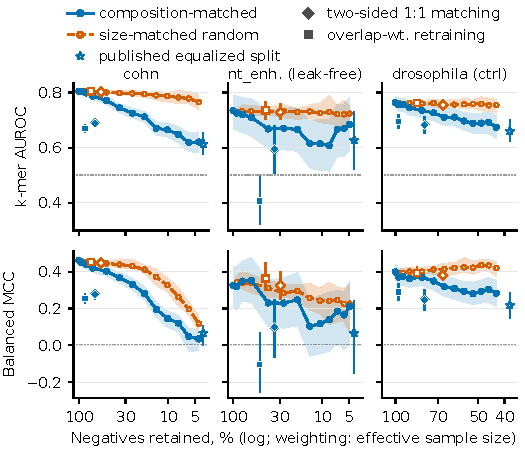
\includegraphics[width=0.62\linewidth]{figs/psm_sensitivity.pdf}
\caption{Composition matching vs.\ size-matched random negatives across matching strictness. $k$-mer
AUROC (top) and balanced MCC (bottom; class-balance-weighted, threshold = training positive
fraction) against the percentage of negatives retained (log scale; for weighting, the effective
sample size). Solid: composition-matched negatives (95\% bootstrap CI; the last point is the
released equalizer rule re-drawn with selection seed 42). Dashed: size-matched random negatives
(10-draw range). Star: the released equalized split (legend: ``published equalized split''). Square:
model retrained with overlap weights
against a permuted-weight placebo. Diamond: two-sided 1:1 caliper-0.2 matching against random 1:1.
Markers are offset in $x$ for legibility. \task{nt\_enh.}: leak-free test (post hoc); its overlap weights
over-correct, so its square lies below chance. Source:
\src{results/upgrades/figures/psm\_sensitivity.pdf}.}
\label{fig:psm}
\end{figure}

\begin{figure}[!htbp]
\centering
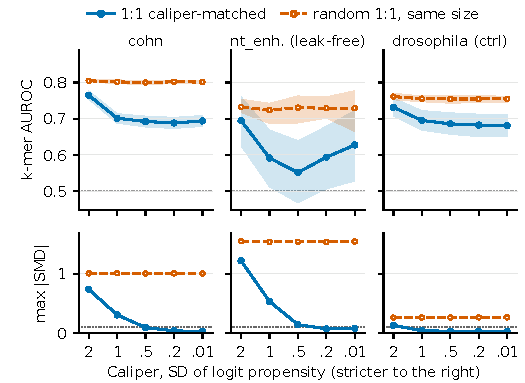
\includegraphics[width=0.62\linewidth]{figs/psm_sensitivity_caliper.pdf}
\caption{Two-sided 1:1 matching across calipers from 2 to 0.01 SD of the logit propensity. Top:
$k$-mer AUROC, matched (95\% CI) against random 1:1 subsets of the same size (10-draw range). Bottom:
max$|$SMD$|$ of the matched set (solid) and of the random subsets (dashed); dotted line 0.1. Source:
\src{results/upgrades/figures/psm\_sensitivity\_caliper.pdf}.}
\label{fig:psmcal}
\end{figure}

\subsection{What matching removes: the GC-balanced control}
Matching also lowers the GC-balanced control (random \smCtlAr, matched \smCtlAm\ \smCtlAmCI;
pre-specified verdict supported). The control has composition signal of its own (composition-only
LightGBM AUROC \smCtlComp), and in the paired designs its composition-only baseline falls as much as
the $k$-mer model does: \smCtlFixedC\ against \smCtlFixedK\ with the model fixed, and \smCtlTrainC\
against \smCtlTrainK\ on the original test. (In the retrained within design with seed 42 the
composition-only loss is smaller, \smCtlWithinC\ \smCtlWithinCCI\ against \smCtlWithinK; over seeds
42--44 the two are \smCtlWithinCS\ and \smCtlWithinKS.) Matching therefore removes
composition-associated signal, artifactual or biological. It is also incomplete: the composition-only
AUROC falls from \smCompZero\ to \smCompPub\ \smCompPubCI\ on the released equalized \task{cohn} split,
not to 0.5.

For \task{cohn} the $k$-mer loss does not exceed the composition-only loss (\smMvrPoint\ against
\smCohnWithinC\ retrained; \smCohnFixedK\ against \smCohnFixedC\ with the model fixed). Across the
matching arms, \task{cohn}'s $k$-mer gap correlates with the composition-only gap more than with
selection depth in all three designs, but by the 0.3-margin reading rule of this post hoc summary the
separation is clear only in the within design (Table~\ref{tab:psmdissoc}). Under overlap weighting \task{cohn} loses a larger share
of its above-chance AUROC than the control (contrast \smBetK), but the composition-only model loses an
equally larger share under the same weights (\smBetC; difference of contrasts \smBetDoc;
Table~\ref{tab:psmbetween}). The contrast measures reliance on the composition gap, not contamination
specificity.

% generated by bibm/supplement/make_sm_tables.py -- do not edit; sources: psm_sensitivity_between_dataset.csv
\begin{table}[!htbp]
\caption{Between-dataset contrast under removal-free overlap weighting: share of above-chance AUROC lost by the $k$-mer model and by the composition-only model under the same weights (post hoc P4/P6). Source: \src{psm\_sensitivity\_between\_dataset.csv}.}
\label{tab:psmbetween}
\centering
\footnotesize
\begin{tabular}{llll}
\toprule
Data & $k$-mer share lost [CI] & Comp.-only share lost [CI] & $k$-mer/comp.-only [CI] \\
\midrule
\multicolumn{4}{@{}l}{\emph{original model, overlap-weighted test}} \\
\task{cohn} & 0.644 [0.606, 0.685] & 0.806 [0.760, 0.855] & 0.80 [0.77, 0.83] \\
GC-balanced control & 0.290 [0.248, 0.336] & 0.454 [0.376, 0.545] & 0.64 [0.52, 0.75] \\
\task{cohn} $-$ control & +0.353 [+0.293, +0.413] & +0.352 [+0.247, +0.442] & diff.\ of contrasts +0.002 [−0.070, +0.088] \\
\multicolumn{4}{@{}l}{\emph{retrained with overlap weights}} \\
\task{cohn} & 0.441 [0.403, 0.477] & 0.622 [0.577, 0.665] & 0.71 [0.64, 0.78] \\
GC-balanced control & 0.257 [0.209, 0.310] & 0.364 [0.278, 0.460] & 0.71 [0.54, 0.95] \\
\task{cohn} $-$ control & +0.183 [+0.119, +0.244] & +0.258 [+0.153, +0.356] & diff.\ of contrasts −0.074 [−0.186, +0.031] \\
\bottomrule
\end{tabular}
\par\smallskip
\begin{minipage}{\linewidth}\footnotesize\raggedright
The $k$-mer contrast between \task{cohn} and the GC-balanced control is matched by the composition-only contrast under the same weights (difference of contrasts near 0), so it measures reliance on the composition gap, not contamination specificity. \task{nt\_enhancers} is omitted: the weights over-correct there (weighted AUROC below 0.5), so its shares ($>$1) are not interpretable.
\end{minipage}
\end{table}

% generated by bibm/supplement/make_sm_tables.py -- do not edit; sources: psm_sensitivity_dissociation_stats.csv
\begin{table}[!htbp]
\caption{Across matching arms, does the $k$-mer gap track the composition signal removed or the selection depth? (post hoc, descriptive). Source: \src{psm\_sensitivity\_dissociation\_stats.csv}.}
\label{tab:psmdissoc}
\centering
\scriptsize
\setlength{\tabcolsep}{3pt}
\begin{tabular}{l>{\raggedright\arraybackslash}p{0.17\linewidth}rrrrr>{\raggedright\arraybackslash}p{0.2\linewidth}}
\toprule
Data & Design & Arms & $\rho$ w/ comp.\ gap & $\rho$ w/ depth & OLS comp. & OLS depth & Reading (0.3-margin rule) \\
\midrule
\task{cohn} & within (retrained, own test) & 24 & +0.96 & +0.39 & +0.045 & +0.016 & gap tracks composition-signal removal more than selection depth \\
 & model fixed (original model) & 24 & +0.98 & +0.71 & +0.061 & +0.005 & no clear separation of composition-signal removal and selection depth \\
 & undistorted test (retrained, original test) & 24 & +0.92 & +0.65 & +0.070 & +0.024 & no clear separation of composition-signal removal and selection depth \\
\task{nt\_enhancers}, leak-free test & within (retrained, own test) & 22 & +0.81 & +0.18 & +0.040 & −0.007 & gap tracks composition-signal removal more than selection depth \\
 & model fixed (original model) & 22 & +0.99 & +0.63 & +0.067 & +0.001 & gap tracks composition-signal removal more than selection depth \\
 & undistorted test (retrained, original test) & 24 & +0.86 & +0.63 & +0.085 & −0.022 & no clear separation of composition-signal removal and selection depth \\
GC-balanced control & within (retrained, own test) & 24 & +0.07 & +0.86 & +0.016 & +0.038 & gap tracks selection depth (-log retention) more than composition-signal removal \\
 & model fixed (original model) & 24 & +0.99 & +0.76 & +0.040 & −0.001 & no clear separation of composition-signal removal and selection depth \\
 & undistorted test (retrained, original test) & 24 & +0.97 & +0.81 & +0.025 & +0.019 & no clear separation of composition-signal removal and selection depth \\
\bottomrule
\end{tabular}
\par\smallskip
\begin{minipage}{\linewidth}\footnotesize\raggedright
Spearman correlation of the $k$-mer gap with the composition-only gap and with selection depth ($-\log$ retained fraction) over the non-underpowered strictness, trimming and caliper arms; OLS: partial coefficients per SD. Arms overlap and the random controls are nested, so no $p$-values are given. For \task{cohn} the correlation with the composition gap is the larger of the two in all three designs, but by the 0.3-margin rule the separation is clear only in the within design.
\end{minipage}
\end{table}


\subsection{Selection bias and label noise}
The kept \task{cohn} negatives match the positives' TATA-box rate (\smTataKept\ against \smTataPos;
discarded \smTataDisc) and are enriched for enhancer-like cCREs~\cite{encode2020} (\smElsKept\ of kept
against \smElsDisc\ of discarded negatives; positives \smElsPos; Bonferroni $p$~=~\smElsP), but not for
TSS overlap after correction (\smTssKept\ against \smTssDisc; $p$~=~\smTssP; Table~\ref{tab:psmselbias}).
If some kept negatives are unlabeled enhancers, the matched AUROC would be too low. Re-scoring
without cCRE-overlapping test negatives keeps the drop (\smCcreFree\ \smCcreFreeCI\ against
\smCcreFreeR, with \smCcreFreeN\ matched test negatives), and a mixture-model estimate (not a
worst case) puts the AUROC cost of hidden enhancers at \smLabelNoise, \smLabelNoiseRatio\ times the
matched-vs-random effect (Table~\ref{tab:psmlabelnoise}).

% generated by bibm/supplement/make_sm_tables.py -- do not edit; sources: psm_sensitivity_selection_bias.csv
\begin{table}[!htbp]
\caption{Selection bias of composition matching on \task{cohn} ($\alpha{=}1$, seed 42): features outside the propensity model in kept vs.\ discarded negatives. Source: \src{psm\_sensitivity\_selection\_bias.csv}.}
\label{tab:psmselbias}
\centering
\footnotesize
\begin{tabular}{lrrrrr}
\toprule
Feature & Kept neg.\ ($n{=}627$) & Discarded (13{,}269) & Random, same size & Positives & Bonferroni $p$ \\
\midrule
TATA-box hit (TBP $\ge$1.3 bits/pos) & 0.346 & 0.585 & 0.576 & 0.352 & 1.4{\texttimes}10\textsuperscript{−29} \\
ENCODE enhancer-like cCRE (ELS) overlap & 0.337 & 0.236 & 0.239 & 0.907 & 5.3{\texttimes}10\textsuperscript{−6} \\
any ENCODE cCRE overlap & 0.512 & 0.382 & 0.391 & 0.940 & 2.3{\texttimes}10\textsuperscript{−8} \\
promoter-like cCRE (PLS) overlap & 0.011 & 0.003 & 0.003 & 0.067 & 0.52 \\
GENCODE v44 TSS $\pm$500\,bp overlap & 0.043 & 0.024 & 0.026 & 0.156 & 0.77 \\
RepeatMasker coverage & 0.539 & 0.552 & 0.555 & 0.286 & 1.0 \\
\bottomrule
\end{tabular}
\par\smallskip
\begin{minipage}{\linewidth}\footnotesize\raggedright
Fisher or Mann--Whitney test of kept vs.\ discarded negatives, Bonferroni-adjusted over 158 tests (part 6, pre-specified). The kept negatives match the positives' TATA rate and are enriched for enhancer-like cCREs, the expected signature if some are unlabeled enhancers; Table~\ref{tab:psmlabelnoise} checks what that could do to the AUROC.
\end{minipage}
\end{table}

% generated by bibm/supplement/make_sm_tables.py -- do not edit; sources: psm_sensitivity_decision.csv
\begin{table}[!htbp]
\caption{Label-noise checks on \task{cohn}: does matching lower AUROC only because kept negatives are unlabeled enhancers? Source: \src{psm\_sensitivity\_decision.csv}.}
\label{tab:psmlabelnoise}
\centering
\footnotesize
\begin{tabular}{>{\raggedright\arraybackslash}p{0.5\linewidth}llr}
\toprule
Check & Matched [CI] & Random & Matched test neg. \\
\midrule
cCRE-overlapping test negatives removed, same models (pre-specified design c) & 0.646 [0.596, 0.696] & 0.817 & 119 \\
Two-sided 1:1 on the cCRE-purged pool (design b; balanced) & 0.755 [0.738, 0.772] & 0.862 & -- \\
Re-matching on the cCRE-purged pool (design a; not balanced) & 0.686 [0.610, 0.762] & 0.779 & -- \\
\bottomrule
\end{tabular}
\par\smallskip
\begin{minipage}{\linewidth}\footnotesize\raggedright
Design (a) keeps 0.9\% of negatives and is not composition-balanced (max$|$SMD$|$ 0.17); design (b) is balanced (max$|$SMD$|$ 0.08). A mixture-model \emph{estimate} (not a worst case) of the AUROC cost of hidden enhancers among the kept negatives is 0.038, 0.26$\times$ the matched-vs-random effect.
\end{minipage}
\end{table}


\subsection{\texorpdfstring{\task{nt\_enhancers}}{nt\textunderscore enhancers}}
\smNtDup\ of the \smNtTest\ \task{nt\_enhancers} test sequences, all of them positives, occur verbatim in
the training split (original AUROC \smNtLeakA; \smNtLeakFreeA\ without them), so we also score a
leak-free test (post hoc) that drops them. At $\alpha{=}1$ the one-sided equalizer keeps
\smNtTestNeg\ test negatives and cannot balance the set (max$|$SMD$|$ \smNtSMD; released equalized split
\smSMDntPub). The pre-specified within-design test, on the original test, fails (matched \smNtPreAm\
against random \smNtPreAr; matched-vs-random \smNtPreWithinD), and so does the same test on the
leak-free test (matched \smNtAm\ against random \smNtAr; \smNtWithinD): the verdict is ``not
supported'' in every \task{nt\_enhancers} variant (Table~\ref{tab:psmdecision}; Fig.~\ref{fig:psmraw} for the
original test). On the leak-free test
(post hoc), with the original model or the original test held fixed, the set loses \smNtFixedD\ and
\smNtTrainD\ AUROC beyond random negatives, and the two-sided 1:1 caliper
design, which does balance \task{nt\_enhancers} (\smCalNtKept\ of each class kept; max$|$SMD$|$
\smCalNtSMD), gives a \task{cohn}-like gap (\smCalNtMatched\ against \smCalNtRand, gap \smCalNtGap). In
each of these designs the composition-only baseline loses at least as much (\smNtFixedComp,
\smNtTrainComp\ and \smCalNtComp). As for \task{cohn}, this is reliance on composition-associated
signal, not contamination specificity; the control's caliper gap is \smCalCtlGap.

\begin{figure}[!htbp]
\centering
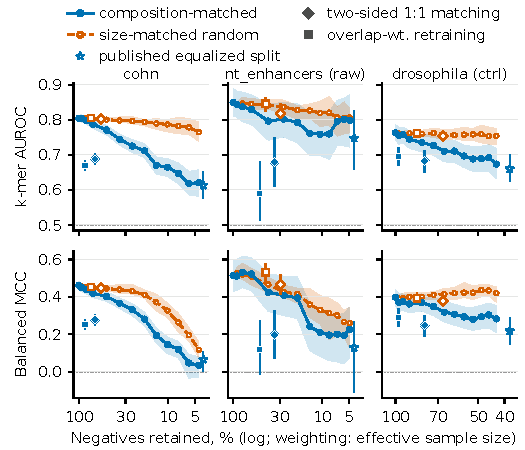
\includegraphics[width=0.62\linewidth]{figs/psm_sensitivity_ntraw.pdf}
\caption{As Fig.~\ref{fig:psm}, with the uncorrected \task{nt\_enhancers} test (\smNtDup\ of its test
positives occur verbatim in training). This original test carries the pre-specified verdict (not
supported); Figs.~\ref{fig:psm} and~\ref{fig:psmcal} use the leak-free test (post hoc). Source:
\src{results/upgrades/figures/psm\_sensitivity\_ntraw.pdf}.}
\label{fig:psmraw}
\end{figure}

\subsection{Why the equalized-split MCC is not used}
Size-matched random negatives reproduce the equalized-split MCC collapse: for the $k$-mer model on
\task{cohn}, random negatives give \smMCCrand\ (range \smMCCrandRange) against \smMCCpub\ on the
released equalized split, from \smMCCzero\ (share reproduced \smMCCshare); for the composition-only
baseline they reproduce \smCompMCCshare\ of its collapse (\smCompMCCzero\ to \smCompMCCrand, against
\smCompMCCpub\ on the released equalized split; Table~\ref{tab:psmmcc}). The released split's \smMCCpub\
is also the largest of \smDraws\ equally valid matching draws (range \smDrawMCC, median \smDrawMCCmed).
Random removal at a retention comparable to the TATA-flag cleaning (\smMCCrandKeptRange\ of negatives
kept) lowers the \task{cohn} MCC by about \smMCCrandDrop\ (\smMCCzero\ to \smMCCrandMin--\smMCCrandMax).

% generated by bibm/supplement/make_sm_tables.py -- do not edit; sources: psm_sensitivity_decision.csv
\begin{table}[!htbp]
\caption{Why the equalized-split MCC is not used: size-matched random negatives reproduce most or all of its collapse (MCC at threshold 0.5). Source: \src{psm\_sensitivity\_decision.csv}.}
\label{tab:psmmcc}
\centering
\scriptsize
\setlength{\tabcolsep}{3pt}
\begin{tabular}{>{\raggedright\arraybackslash}p{0.2\linewidth}rlrrrrrr}
\toprule
 & \multicolumn{4}{c}{$k$-mer LightGBM} & \multicolumn{4}{c}{composition-only LightGBM} \\
Data & Original & Random (range) & Released split & Share & Original & Random & Released split & Share \\
\midrule
\task{cohn} & 0.461 & 0.022 (0.000--0.091) & 0.064 & 1.11 & 0.410 & 0.144 & 0.000 & 0.65 \\
\task{nt\_enhancers}, leak-free test & 0.311 & 0.191 (0.065--0.290) & 0.000 & 0.39 & 0.310 & 0.131 & 0.060 & 0.72 \\
GC-balanced control & 0.398 & 0.425 (0.398--0.477) & 0.177 & −0.12 & 0.253 & 0.257 & 0.049 & −0.02 \\
\bottomrule
\end{tabular}
\par\smallskip
\begin{minipage}{\linewidth}\footnotesize\raggedright
Share = (original $-$ random)/(original $-$ released equalized split), the share of the collapse that size-matched random negatives reproduce. On the \task{cohn} test set, which is about 94\% positive at this retention, a model trained on about 96\% positives predicts almost everything positive, so MCC at 0.5 mostly measures the size/imbalance change. Over the 20 equally valid matching draws of the released equalizer on \task{cohn}, the equalized $k$-mer MCC ranges 0.000--0.064 (median 0.000; \task{homology\_recluster\_e1\_draws\_summary.csv}). In the balanced 1:1 design MCC isolates the matched-vs-random contrast at caliper 0.2 SD: 0.277 vs.\ 0.448 for random 1:1 subsets (\task{psm\_sensitivity\_caliper\_sweep.csv}).
\end{minipage}
\end{table}


\subsection{Dinucleotide-shuffled negatives}
Against dinucleotide-preserving shuffles of the positives~\cite{altschul1985} (no mono- or
dinucleotide composition gap by construction), the negative-class TATA skew disappears
(\task{cohn} TATA AUROC \smShufTata; \smShufTataRange\ over \smHashDraws\ shuffle draws), while the positives remain
separable from their own shuffles by higher-order structure ($k$-mer AUROC \smShufKmerCohn\ and
\smShufKmerNt; Table~\ref{tab:shuffle}). The skew is thus a by-product of the composition gap. Like
matching, the shuffle does not separate artifactual from biological composition. The shuffle depends
on \task{PYTHONHASHSEED}, and the paper's exact draw was not recovered by the \smHashDraws-draw scan.

% generated by bibm/supplement/make_sm_tables.py -- do not edit; sources: shuffled_neg.csv, alt_model_shuffle_hashseed.csv
\begin{table}[!htbp]
\caption{Dinucleotide-shuffled negatives: the paper's draw and the range over 16 \task{PYTHONHASHSEED} draws of the shuffle. Source: \src{shuffled\_neg.csv},\enspace \src{alt\_model\_shuffle\_hashseed.csv}.}
\label{tab:shuffle}
\centering
\scriptsize
\setlength{\tabcolsep}{3pt}
\begin{tabular}{lllllll}
\toprule
 & \multicolumn{2}{c}{TATA motif-only AUROC} &  &  &  &  \\
Data & real neg. & shuffled (range) & GC-content AUROC & $k$-mer AUROC (range) & $k$-mer MCC (range) & = paper \\
\midrule
\task{cohn} & 0.371 & 0.551 (0.549--0.554) & 0.500 & 0.955 (0.951--0.955) & 0.769 (0.759--0.776) & 0/16 \\
\task{nt\_enhancers} & 0.393 & 0.507 (0.503--0.510) & 0.500 & 0.856 (0.839--0.879) & 0.545 (0.520--0.627) & 0/16 \\
control & 0.539 & 0.749 (0.746--0.754) & 0.500 & 0.989 (0.988--0.996) & 0.922 (0.906--0.937) & 0/16 \\
\bottomrule
\end{tabular}
\par\smallskip
\begin{minipage}{\linewidth}\footnotesize\raggedright
Shuffles of the positives remove the mono- and dinucleotide composition gap by construction (GC-content AUROC 0.500 on every task; the GC-content AUROC is that of per-sequence GC content, not a motif score). The negative-class TATA skew disappears (\task{cohn} TATA AUROC slightly above 0.5 in every draw), while the positives remain separable from their own shuffles by higher-order structure; for the control, whose TATA is a positive-class motif, the TATA AUROC rises. All sequences are scanned. The shuffle depends on \task{PYTHONHASHSEED}; the paper's exact draw was not recovered by the 16-seed scan.
\end{minipage}
\end{table}


\subsection{Control-motif panel}\label{sec:s4ctl}
Fig.~\ref{fig:ctlmotif} and Table~\ref{tab:ctlmotif} give the control-motif panel. Random PWMs matched to the TBP information content produce no class skew
(motif-only AUROC \smRandICcohn\ on \task{cohn}), so the scan does not manufacture one;
column-scrambled TBP PWMs keep the TBP columns' AT-rich composition but not the ordered TATA pattern,
and stay skewed. The skew is therefore composition-driven, not a scan artifact. The panel does not
show contamination specificity.

% generated by bibm/supplement/make_sm_tables.py -- do not edit; sources: route3_specificity.csv, route3_threshold_invariance.csv
\begin{table}[!htbp]
\caption{Control-motif panel (motif-only AUROC at 1.3 bits/pos; mean $\pm$ SD over the panel, or estimate [95\% CI]) and threshold invariance of the TATA skew. Source: \src{route3\_specificity.csv},\enspace \src{route3\_threshold\_invariance.csv}.}
\label{tab:ctlmotif}
\centering
\footnotesize
\begin{tabular}{llr}
\toprule
Data & Motif & Motif-only AUROC \\
\midrule
\task{cohn} & real TATA (TBP PSSM) & 0.367 [0.356, 0.378] \\
\task{cohn} & column-scrambled TBP (20 PWMs) & 0.376 $\pm$ 0.017 \\
\task{cohn} & IC-matched random PWMs (10) & 0.502 $\pm$ 0.033 \\
\task{nt\_enhancers} & real TATA (TBP PSSM) & 0.392 [0.383, 0.400] \\
\task{nt\_enhancers} & column-scrambled TBP (20 PWMs) & 0.396 $\pm$ 0.027 \\
\task{nt\_enhancers} & IC-matched random PWMs (10) & 0.507 $\pm$ 0.016 \\
\task{nt\_prom\_tata} & real TATA (TBP PSSM) & 0.589 [0.577, 0.600] \\
\midrule
\task{cohn} & TATA AUROC over 0.8--1.5 bits/pos: original / equalized & 0.307--0.401 / 0.485--0.503 \\
\task{nt\_enhancers} & TATA AUROC over 0.8--1.5 bits/pos: original / equalized & 0.282--0.431 / 0.490--0.501 \\
\bottomrule
\end{tabular}
\par\smallskip
\begin{minipage}{\linewidth}\footnotesize\raggedright
An AUROC below 0.5 means the motif is commoner in the negatives. Random PWMs matched to the TBP information content produce no class skew, so the scan does not manufacture one; column-scrambled TBP PWMs keep the TBP columns' AT-rich composition but not the ordered TATA pattern and stay skewed, so the skew is composition-driven. Real TATA on \task{nt\_promoter\_tata} is skewed toward the positives (positive control). The panel was re-run on homology-clean data (\task{homology\_recluster\_extra\_specificity.csv}); see Table~\ref{tab:homroutes}. Both panels scan a seeded sample of at most 4{,}000 sequences per class (the equalized splits keep fewer negatives); on all sequences the real-TATA AUROC of the original split is 0.371 (\task{cohn}) and 0.393 (\task{nt\_enhancers}; Table~\ref{tab:shuffle}).
\end{minipage}
\end{table}


\begin{figure}[!htbp]
\centering
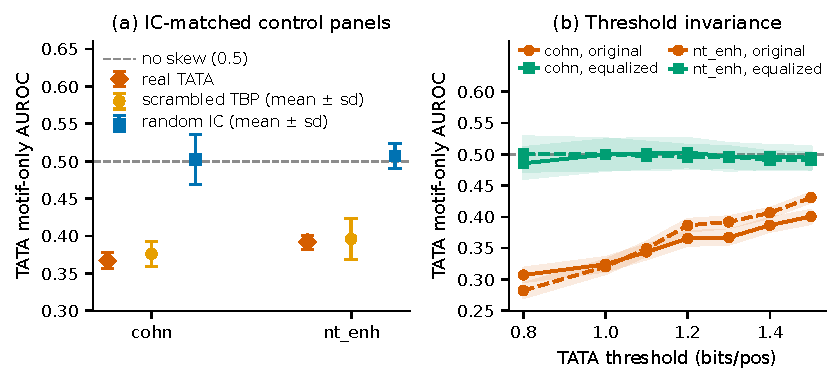
\includegraphics[width=0.8\linewidth]{figs/route3_control_motif_panel.pdf}
\caption{Control-motif panel (data and sources as in Table~\ref{tab:ctlmotif}; seed 42; at most \smTataSampleN\
sequences per class). (a) TATA motif-only AUROC (positives $>$ negatives) of the real TBP PSSM (95\% CI),
\smNscr\ column-scrambled TBP PWMs (composition kept, order destroyed) and \smNric\ random PWMs matched to
TBP's information content (both mean $\pm$ SD), on \task{cohn} and \task{nt\_enhancers} (\task{nt\_enh});
dashed line: no skew. (b) The same AUROC across 0.8--1.5 bits/pos on the original and the released
equalized splits (95\% bootstrap bands). Re-plot of \src{results/upgrades/figures/route3\_specificity.pdf}
(same code and data) with the legend of (b) moved.}
\label{fig:ctlmotif}
\end{figure}

% =====================================================================
\section{FM probes, frozen and fine-tuned}\label{sec:s5}

\subsection{Frozen probes}
A frozen probe's \emph{test effect} is the AUROC change of the same fixed head when composition-biased
test negatives are removed (negative = loss), leaving the GC-matched subset (test negatives subsampled to
the positives' GC histogram; the paper's GC-matched intervention). It is significant for both
FMs on both contaminated sets, for both heads and under both poolings (Table~\ref{tab:frozen},
Fig.~\ref{fig:frozen}). Whether the GC-balanced control is flat depends on the pooling: it is flat
under HyenaDNA's [SEP] token (\smFrozCtlSep), not under mean pooling (\smFrozCtlMean). The small
test effect is a floor: on composition-equalized negatives the same models lose
\smFloorLo--\smFloorHi\ \task{cohn} AUROC, frozen or fine-tuned (Table~\ref{tab:ftcompare}), a loss that
also includes genuine composition signal.

% generated by bibm/supplement/make_sm_tables.py -- do not edit; sources: fm_head_invariance.csv, fm_cross_architecture.csv
\begin{table}[!htbp]
\caption{Frozen FM probes: test effect, the AUROC change of the same fixed head (negative = loss) when composition-biased test negatives are removed (GC-matched arm), by pooling and head. Source: \src{fm\_head\_invariance.csv},\enspace \src{fm\_cross\_architecture.csv}.}
\label{tab:frozen}
\centering
\footnotesize
\begin{tabular}{llllll}
\toprule
Model & Data & Pooling & Head & Test effect [95\% CI] & CI excludes 0 \\
\midrule
HyenaDNA-tiny & \task{cohn} & [SEP] & LightGBM & −0.0481 [−0.053, −0.043] & yes \\
HyenaDNA-tiny & \task{cohn} & [SEP] & LR & −0.0502 [−0.056, −0.045] & yes \\
HyenaDNA-tiny & \task{cohn} & mean & LightGBM & −0.0575 [−0.063, −0.052] & yes \\
HyenaDNA-tiny & \task{cohn} & mean & LR & −0.0727 [−0.079, −0.067] & yes \\
HyenaDNA-tiny & \task{nt\_enhancers} & [SEP] & LightGBM & −0.0793 [−0.107, −0.056] & yes \\
HyenaDNA-tiny & \task{nt\_enhancers} & [SEP] & LR & −0.0971 [−0.128, −0.067] & yes \\
HyenaDNA-tiny & \task{nt\_enhancers} & mean & LightGBM & −0.0799 [−0.108, −0.055] & yes \\
HyenaDNA-tiny & \task{nt\_enhancers} & mean & LR & −0.1243 [−0.159, −0.093] & yes \\
HyenaDNA-tiny & control & [SEP] & LightGBM & +0.0055 [−0.003, +0.014] & no \\
HyenaDNA-tiny & control & [SEP] & LR & +0.0040 [−0.004, +0.013] & no \\
HyenaDNA-tiny & control & mean & LightGBM & −0.0385 [−0.047, −0.030] & yes \\
HyenaDNA-tiny & control & mean & LR & −0.0188 [−0.033, −0.006] & yes \\
DNABERT-2-117M & \task{cohn} & mean & LightGBM & −0.0467 [−0.051, −0.042] & yes \\
DNABERT-2-117M & \task{cohn} & mean & LR & −0.0486 [−0.053, −0.044] & yes \\
DNABERT-2-117M & \task{cohn} & [CLS] & LightGBM & −0.0465 [−0.052, −0.042] & yes \\
DNABERT-2-117M & \task{cohn} & [CLS] & LR & −0.0472 [−0.052, −0.043] & yes \\
DNABERT-2-117M & \task{nt\_enhancers} & mean & LightGBM & −0.0720 [−0.100, −0.049] & yes \\
DNABERT-2-117M & \task{nt\_enhancers} & mean & LR & −0.0939 [−0.126, −0.065] & yes \\
DNABERT-2-117M & \task{nt\_enhancers} & [CLS] & LightGBM & −0.0771 [−0.106, −0.051] & yes \\
DNABERT-2-117M & \task{nt\_enhancers} & [CLS] & LR & −0.0921 [−0.125, −0.063] & yes \\
\bottomrule
\end{tabular}
\par\smallskip
\begin{minipage}{\linewidth}\footnotesize\raggedright
Nested paired bootstrap. The effect has the same sign and significance for both heads under each pooling (head-invariant). Whether the GC-balanced control (\task{drosophila\_enhancers\_stark}) is flat depends on the pooling: it is flat under the [SEP] token only. DNABERT-2 was not run on the control; its flat reference in the paper is a placebo that removes as many \task{cohn} test negatives at random.
\end{minipage}
\end{table}


\begin{figure}[!htbp]
\centering
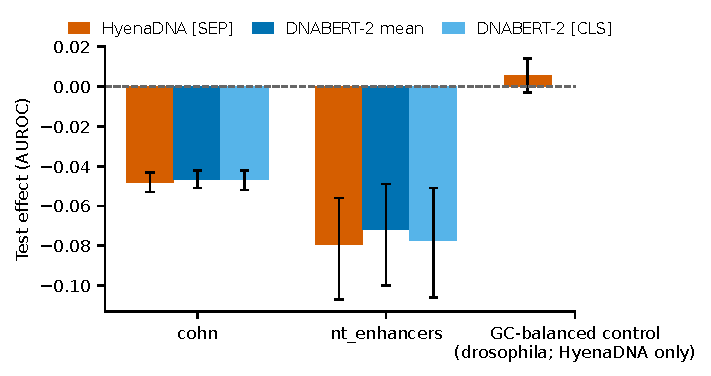
\includegraphics[width=0.69\linewidth]{figs/fm_frozen_probe.pdf}
\caption{Frozen FM probes: test effect (AUROC change, negative = loss; Section~\ref{sec:s5}) of the fixed LightGBM head on the
GC-matched arm for HyenaDNA ([SEP] token) and DNABERT-2 (mean and [CLS] pooling), with 95\% bootstrap
CIs (data as in Table~\ref{tab:frozen}). The GC-balanced control (\task{drosophila}) was probed with
HyenaDNA only, [SEP] token. Seed 42. Re-plotted for this supplement from
\src{fm\_cross\_architecture.csv}; same data as \src{results/upgrades/figures/fm\_cross\_architecture.png}.}
\label{fig:frozen}
\end{figure}

\subsection{End-to-end fine-tuning}\label{sec:s5ft}
Two FMs were fine-tuned end to end, \smNunits\ units in total: HyenaDNA-tiny-16k-d128~\cite{hyenadna}
with all \smFTHParams\ parameters trainable (AdamW, learning rate $6\times10^{-4}$, 6 epochs), and
DNABERT-2-117M~\cite{dnabert2} with LoRA~\cite{hu2022} (rank 8, $\alpha=16$, on the attention and GLU
layers; \smFTDParams\ parameters trainable, \smFTDParamsPct; AdamW, $3\times10^{-4}$, at most 4 epochs
with early stopping). Each has a linear head on mean-pooled states and class-weighted cross-entropy;
the epoch is chosen on a 10\% validation carve of the training split; seeds 42--44; one fixed recipe
per model, with no hyperparameter search. Every model scores the whole original test split, so the
arms are the same weights scored on different test negatives: original ($A$), composition-equalized
($B$) and a size-matched random subset of the original negatives ($C$). Models retrained on equalized
($D$) or random ($E$) negatives are also reported. The contrasts and rules were fixed before any unit
finished; the share of above-chance AUROC lost is a post hoc re-expression.

On \task{cohn} both models lose AUROC on equalized test negatives and nothing on random ones
(Table~\ref{tab:ft}): HyenaDNA \smFTHA\ to \smFTHB\ (random \smFTHC) and DNABERT-2 \smFTDA\ to \smFTDB\
(random \smFTDC; by arm in Fig.~\ref{fig:ftarms}). Re-expressed, that is \smFTHShare\ and \smFTDShare\ of the
above-chance AUROC (Fig.~\ref{fig:ftcompare}).
Fine-tuned HyenaDNA's share is not significantly different from the $k$-mer model's in the same design
(\smFTKmerShare; paired difference \smFTHvsKmer), and LoRA reduces but does not remove the reliance.
Rule~1 is met for HyenaDNA only through its $B<0.6$ clause and is not met for DNABERT-2
(Table~\ref{tab:ftrules}). $B$ is not a chance draw of a small negative set: it lies below all 1000
random draws of as many negatives (Table~\ref{tab:ftranddraw}).

% generated by bibm/supplement/make_sm_tables.py -- do not edit; sources: fm_finetune_v2_paper_table.csv, fm_finetune_v2_unit_diagnostics.csv
\begin{table}[!htbp]
\caption{End-to-end fine-tuning (seed means over 42--44): the same weights scored on original ($A$), composition-equalized ($B$) and size-matched random ($C$) test negatives; $D$/$E$: retrained on equalized/random negatives. Source: \src{fm\_finetune\_v2\_paper\_table.csv},\enspace \src{fm\_finetune\_v2\_unit\_diagnostics.csv}.}
\label{tab:ft}
\centering
\scriptsize
\setlength{\tabcolsep}{1.8pt}
\begin{tabular}{llllllllll}
\toprule
Model & Data & $A$ & $B$ [CI] & $C$ & $D$ & $E$ & $S{=}A{-}B$ [CI] & $T{=}C{-}B$ [CI] & Share lost [CI] (random) \\
\midrule
HyenaDNA-tiny, full & \task{cohn} & 0.796 & 0.581 [0.542, 0.618] & 0.804 & 0.522$^\ast$ & 0.775 & +0.214 [+0.180, +0.252] & +0.223 [+0.181, +0.271] & 72\% [60, 86] (−3\%) \\
DNABERT-2, LoRA & \task{cohn} & 0.848 & 0.720 [0.683, 0.752] & 0.863 & 0.703 & 0.833 & +0.128 [+0.095, +0.161] & +0.143 [+0.103, +0.183] & 37\% [27, 46] (−4\%) \\
HyenaDNA-tiny, full & \task{nt\_enhancers} & 0.762 & 0.593 [0.504, 0.684] & 0.797 & 0.643 & 0.822 & +0.169 [+0.095, +0.241] & +0.204 [+0.099, +0.309] & 64\% [35, 98] (−13\%) \\
DNABERT-2, LoRA & \task{nt\_enhancers} & 0.820 & 0.680 [0.592, 0.773] & 0.833 & 0.693 & 0.816 & +0.140 [+0.069, +0.216] & +0.153 [+0.049, +0.265] & 44\% [20, 70] (−4\%) \\
HyenaDNA-tiny, full & control & 0.828 & 0.742 [0.707, 0.779] & 0.846 & 0.726 & 0.819 & +0.086 [+0.056, +0.114] & +0.105 [+0.065, +0.142] & 26\% [17, 35] (−6\%) \\
\bottomrule
\end{tabular}
\par\smallskip
\begin{minipage}{\linewidth}\footnotesize\raggedright
AUROC; CIs from 1000 resamples of the original test sequences, jointly across arms and averaged over seeds. Share lost $=(A{-}B)/(A{-}0.5)$, the share of above-chance AUROC lost (post hoc re-expression of the pre-specified $S$); random share $=(A{-}C)/(A{-}0.5)$, in parentheses. $^\ast$ all three retrained units are degenerate one-class fits (every test probability $\ge$0.5), so this $D$ is not evidence that the equalized arm is unlearnable. Rule verdicts are in Table~\ref{tab:ftrules}.
\end{minipage}
\end{table}

% generated by bibm/supplement/make_sm_tables.py -- do not edit; sources: fm_finetune_v2_paper_table.csv
\begin{table}[!htbp]
\caption{Pre-specified fine-tuning decision rules, as evaluated. Source: \src{fm\_finetune\_v2\_paper\_table.csv}.}
\label{tab:ftrules}
\centering
\scriptsize
\setlength{\tabcolsep}{3pt}
\begin{tabular}{ll>{\raggedright\arraybackslash}p{0.11\linewidth}>{\raggedright\arraybackslash}p{0.11\linewidth}>{\raggedright\arraybackslash}p{0.22\linewidth}>{\raggedright\arraybackslash}p{0.1\linewidth}}
\toprule
Model & Data & 1: rides the shortcut & 2: drop not a test-imbalance artifact & 3: cause of the retrained collapse & 5: control not destroyed \\
\midrule
HyenaDNA-tiny, full & \task{cohn} & met & met & composition removal (random arm preserves signal) & -- \\
DNABERT-2, LoRA & \task{cohn} & not met & met & composition removal (random arm preserves signal) & -- \\
HyenaDNA-tiny, full & \task{nt\_enhancers} & met & met & composition removal (random arm preserves signal) & -- \\
DNABERT-2, LoRA & \task{nt\_enhancers} & not met & met & composition removal (random arm preserves signal) & -- \\
HyenaDNA-tiny, full & control & not met & met & composition removal (random arm preserves signal) & not met \\
\bottomrule
\end{tabular}
\par\smallskip
\begin{minipage}{\linewidth}\footnotesize\raggedright
Rule 1: $S{>}0$ (CI excludes 0) and either $B$'s CI covers 0.5 or $B{<}0.6$; for HyenaDNA it is met only through $B{<}0.6$ ($B$'s CI excludes 0.5). Rule 2: $T{>}0$ (CI excludes 0) and $C$'s CI overlaps $A$'s. Rule 3 reads $U{=}E{-}D$ and $R$; for HyenaDNA on \task{cohn} it rests on degenerate retrains (Table~\ref{tab:ft}). Rule 5 (GC-balanced control not destroyed): $B$ and $D$ stay above chance (CIs above 0.5) and the control's $S$ lies below that of each contaminated set (its CI upper bound below the other CI's lower bound). Not met: $B$ and $D$ stay above chance, but the control's $S$, +0.086 [+0.056, +0.114], overlaps that of \task{nt\_enhancers}, +0.169 [+0.095, +0.241]. For \task{nt\_enhancers} the retrain-side reading is not used, because the matching test there is not supported (Table~\ref{tab:psmdecision}).
\end{minipage}
\end{table}


The equalizer keeps more cCRE-overlapping negatives than the random control does (\task{cohn} test
negatives: \smCcreEq\ against \smCcreRand; Table~\ref{tab:ftccre}). Without them the \task{cohn} drop
shrinks but persists (\smCcreFTH\ and \smCcreFTD\ of the above-chance AUROC). On \task{nt\_enhancers}
(\smFTNtEqNeg\ equalized test negatives) both models lose AUROC (HyenaDNA \smFTNtH; DNABERT-2 \smFTNtD), but
without cCRE-overlapping negatives the loss is no longer separable from the random control ($T$ CIs
\smCcreNtTH\ and \smCcreNtTD; Table~\ref{tab:ftccrefree}), so the fine-tuned drop is established for
\task{cohn} only.

The GC-balanced control also loses \smFTCtlShare\ of its above-chance AUROC (HyenaDNA only). The
pre-specified rule~5 (the control's $B$ and $D$ above chance and its $S$ below that of each contaminated set, with
disjoint CIs) is not met: $B$ and $D$ stay above chance, but its $S$, \smFTCtlS, overlaps that of
\task{nt\_enhancers}, \smFTNtS\ (Table~\ref{tab:ftrules}). After fine-tuning, the control's GC-matched test
effect is also no longer flat (\smFTCtlGA;
Table~\ref{tab:ftgc}). Fine-tuning, like matching, shows reliance on composition-associated signal,
not that the signal is an artifact. Post hoc, on the leak-free \task{nt\_enhancers} test the drop
persists but carries the cCRE caveat, and on homology-clean data fine-tuned HyenaDNA still loses
\smHcFTS\ on \task{cohn}, while on the homology-clean \task{nt\_enhancers} re-split its GC-matched
shortcut vanishes ($S_\mathrm{gc}$ \smHcFTSgc; Table~\ref{tab:ftposthoc}).

\emph{Caveats.} All three HyenaDNA \task{cohn} models retrained on equalized negatives collapsed to
one-class predictors, so their $D$ is not evidence that the arm is unlearnable. Fine-tuned HyenaDNA
reaches a \task{cohn} accuracy of \smFTBalAcc\ against 0.742 published for the same architecture after a
sweep~\cite{hyenadna}, and an \task{nt\_enhancers} MCC of \smFTNtMCC\ against 0.626 published for a
larger (1.6M) HyenaDNA~\cite{hyenadna}; the models are not leaderboard-tuned. On \task{nt\_enhancers}
\smValLeakMin--\smValLeakMax\ of validation rows have an exact copy among the fitting rows, so
validation AUROC overstates test AUROC (per-model means \smValAucH\ against \smTestAucH\ for HyenaDNA,
\smValAucD\ against \smTestAucD\ for DNABERT-2); the test split is never used for selection. The only
full-parameter model is the \smFTHParamsM-parameter HyenaDNA-tiny; full-parameter DNABERT-2 and NT-v2-500M runs
are packaged but not run (Section~\ref{sec:s9}), and DNABERT-2 was not run on the GC-balanced control
(Section~\ref{sec:s1tok}).

% generated by bibm/supplement/make_sm_tables.py -- do not edit; sources: fm_finetune_v2_compare.csv, fm_finetune_v2_compare_paired.csv
\begin{table}[!htbp]
\caption{One design, three model families on \task{cohn}: the same test sets for the $k$-mer model, the frozen probes and the fine-tuned FMs (post hoc, descriptive). Source: \src{fm\_finetune\_v2\_compare.csv},\enspace \src{fm\_finetune\_v2\_compare\_paired.csv}.}
\label{tab:ftcompare}
\centering
\footnotesize
\begin{tabular}{lllllr}
\toprule
Model & $A$ & $B$ [CI] & $C$ & $S$ & Share lost [CI] \\
\midrule
$k$-mer LightGBM & 0.805 & 0.603 [0.564, 0.639] & 0.820 & +0.202 & 66\% [55, 79] \\
HyenaDNA frozen [SEP] & 0.723 & 0.577 [0.536, 0.614] & 0.740 & +0.146 & 66\% [50, 83] \\
HyenaDNA frozen mean & 0.790 & 0.621 [0.580, 0.660] & 0.802 & +0.169 & 58\% [46, 72] \\
HyenaDNA fine-tuned (full) & 0.796 & 0.581 [0.542, 0.618] & 0.804 & +0.214 & 72\% [60, 86] \\
DNABERT-2 frozen mean & 0.831 & 0.688 [0.650, 0.724] & 0.841 & +0.142 & 43\% [33, 54] \\
DNABERT-2 frozen [CLS] & 0.804 & 0.672 [0.632, 0.709] & 0.814 & +0.132 & 44\% [32, 56] \\
DNABERT-2 fine-tuned (LoRA) & 0.848 & 0.720 [0.683, 0.752] & 0.863 & +0.128 & 37\% [27, 46] \\
\midrule
HyenaDNA fine-tuned (full) $-$ $k$-mer LightGBM &  &  &  &  & +0.063 [−0.007, +0.135] \\
HyenaDNA fine-tuned (full) $-$ HyenaDNA frozen [SEP] &  &  &  &  & +0.069 [−0.084, +0.218] \\
HyenaDNA fine-tuned (full) $-$ HyenaDNA frozen mean &  &  &  &  & +0.141 [+0.052, +0.238] \\
DNABERT-2 fine-tuned (LoRA) $-$ DNABERT-2 frozen mean &  &  &  &  & −0.061 [−0.109, −0.013] \\
DNABERT-2 fine-tuned (LoRA) $-$ $k$-mer LightGBM &  &  &  &  & −0.293 [−0.387, −0.213] \\
\bottomrule
\end{tabular}
\par\smallskip
\begin{minipage}{\linewidth}\footnotesize\raggedright
Lower block: paired differences of the share lost (same resamples). The $k$-mer share here is in the fine-tuning design; the overlap-weighting design of Section~\ref{sec:s4} gives a different $k$-mer share, so the design is always named. Non-fine-tuned baselines are single deterministic fits on the full training arm.
\end{minipage}
\end{table}


\begin{figure}[!htbp]
\centering
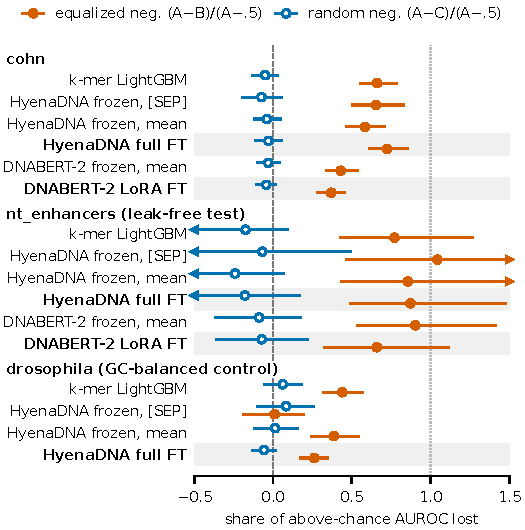
\includegraphics[width=0.55\linewidth]{figs/fm_finetune_v2_compare.pdf}
\caption{Share of above-chance AUROC lost when the same weights are scored on composition-equalized
test negatives, $(A-B)/(A-0.5)$ (filled), and on size-matched random test negatives, $(A-C)/(A-0.5)$
(open), for the $k$-mer model, frozen probes and fine-tuned FMs (post hoc, descriptive; 95\% CIs).
\task{nt\_enhancers} is on its leak-free test (\smFTNtEqNeg\ equalized negatives; wide intervals, some past 1);
\task{drosophila} is the GC-balanced control. The cCRE caveat of Table~\ref{tab:ftccrefree} applies.
Source: \src{results/upgrades/figures/fm\_finetune\_v2\_compare.pdf}.}
\label{fig:ftcompare}
\end{figure}

% generated by bibm/supplement/make_sm_tables.py -- do not edit; sources: fm_finetune_v2_ccre_enrichment.csv
\begin{table}[!htbp]
\caption{Equalized test negatives overlap ENCODE cCREs more often than size-matched random test negatives (post hoc Q3). Source: \src{fm\_finetune\_v2\_ccre\_enrichment.csv}.}
\label{tab:ftccre}
\centering
\footnotesize
\begin{tabular}{llllll}
\toprule
Data & Annotation & Equalized neg.\ overlapping & Random neg. & Positives & Fisher $p$ \\
\midrule
\task{cohn} & any cCRE & 115/228 (50\%) & 32\% & 93\% & 6.0{\texttimes}10\textsuperscript{−5} \\
\task{cohn} & enhancer-like (ELS) & 76/228 (33\%) & 21\% & 91\% & 0.0030 \\
\task{nt\_enhancers} & any cCRE & 14/36 (39\%) & 14\% & 84\% & 0.031 \\
\task{nt\_enhancers} & enhancer-like (ELS) & 9/36 (25\%) & 8\% & 76\% & 0.11 \\
\bottomrule
\end{tabular}
\par\smallskip
\begin{minipage}{\linewidth}\footnotesize\raggedright
The leak-free \task{nt\_enhancers} test has the same 36 equalized negatives. cCRE overlap is itself composition-correlated (positives overlap far more often), so removing cCRE-overlapping negatives also removes the most positive-like negatives; the cCRE-free shares below are a conservative sensitivity analysis, not the `true' composition share.
\end{minipage}
\end{table}

% generated by bibm/supplement/make_sm_tables.py -- do not edit; sources: fm_finetune_v2_ccre_sensitivity.csv
\begin{table}[!htbp]
\caption{Fine-tuned and $k$-mer models re-scored without cCRE-overlapping test negatives (post hoc Q3). Source: \src{fm\_finetune\_v2\_ccre\_sensitivity.csv}.}
\label{tab:ftccrefree}
\centering
\scriptsize
\setlength{\tabcolsep}{3pt}
\begin{tabular}{lllllll}
\toprule
Data & Model & $B$ neg. & $B$ [CI] & $S$ [CI] & $T$ [CI] & Share lost \\
\midrule
cohn & HyenaDNA fine-tuned (full) & 113 & 0.654 [0.604, 0.701] & +0.194 [+0.149, +0.242] & +0.174 [+0.125, +0.228] & 56\% (unfiltered 72\%) \\
 & DNABERT-2 fine-tuned (LoRA) & 113 & 0.804 [0.762, 0.842] & +0.098 [+0.063, +0.135] & +0.101 [+0.059, +0.144] & 24\% (unfiltered 37\%) \\
 & $k$-mer LightGBM & 113 & 0.696 [0.648, 0.742] & +0.164 [+0.121, +0.210] & +0.166 [+0.116, +0.215] & 46\% (unfiltered 66\%) \\
nt\_enhancers & HyenaDNA fine-tuned (full) & 22 & 0.691 [0.578, 0.789] & +0.105 [+0.020, +0.204] & +0.109 [−0.000, +0.227] & 35\% (unfiltered 64\%) \\
 & DNABERT-2 fine-tuned (LoRA) & 22 & 0.774 [0.670, 0.870] & +0.078 [+0.001, +0.170] & +0.065 [−0.045, +0.192] & 22\% (unfiltered 44\%) \\
 & $k$-mer LightGBM & 22 & 0.803 [0.726, 0.873] & +0.075 [+0.022, +0.138] & +0.095 [+0.028, +0.167] & 20\% (unfiltered 43\%) \\
nt\_enhancers\_leakfree & HyenaDNA fine-tuned (full) & 22 & 0.618 [0.495, 0.731] & +0.113 [+0.033, +0.211] & +0.120 [+0.008, +0.238] & 49\% (unfiltered 87\%) \\
 & DNABERT-2 fine-tuned (LoRA) & 22 & 0.677 [0.559, 0.784] & +0.098 [+0.011, +0.189] & +0.091 [−0.027, +0.224] & 36\% (unfiltered 66\%) \\
 & $k$-mer LightGBM & 22 & 0.652 [0.536, 0.762] & +0.118 [+0.040, +0.209] & +0.146 [+0.043, +0.258] & 44\% (unfiltered 77\%) \\
\bottomrule
\end{tabular}
\par\smallskip
\begin{minipage}{\linewidth}\footnotesize\raggedright
On \task{cohn} both $S$ and $T$ exclude 0 for every model. On \task{nt\_enhancers} (22 cCRE-free equalized negatives) $S$ stays positive but $T$'s CI includes 0 for both fine-tuned models, so there the loss is no longer separable from the size-matched random control; the fine-tuned drop is established for \task{cohn} only.
\end{minipage}
\end{table}

% generated by bibm/supplement/make_sm_tables.py -- do not edit; sources: fm_finetune_v2_randdraw.csv
\begin{table}[!htbp]
\caption{Is $B$ a chance draw of a small negative set? 1000 random draws of as many test negatives as the equalized arm holds, with the same positives (post hoc Q4). Source: \src{fm\_finetune\_v2\_randdraw.csv}.}
\label{tab:ftranddraw}
\centering
\footnotesize
\begin{tabular}{llrrlrr}
\toprule
Data & Model & Neg.\ per draw & $B$ & Draw min (2.5--97.5\%) & $C$ & Draws $\le B$ \\
\midrule
cohn & HyenaDNA fine-tuned (full) & 228 & 0.581 & 0.753 (0.768--0.824) & 0.804 & 0 \\
cohn & DNABERT-2 fine-tuned (LoRA) & 228 & 0.720 & 0.803 (0.822--0.870) & 0.863 & 0 \\
nt\_enhancers & HyenaDNA fine-tuned (full) & 36 & 0.593 & 0.634 (0.690--0.822) & 0.797 & 0 \\
nt\_enhancers & DNABERT-2 fine-tuned (LoRA) & 36 & 0.680 & 0.702 (0.752--0.880) & 0.833 & 0 \\
nt\_enhancers\_leakfree & HyenaDNA fine-tuned (full) & 36 & 0.525 & 0.582 (0.624--0.761) & 0.732 & 0 \\
nt\_enhancers\_leakfree & DNABERT-2 fine-tuned (LoRA) & 36 & 0.582 & 0.620 (0.668--0.805) & 0.756 & 0 \\
drosophila & HyenaDNA fine-tuned (full) & 217 & 0.742 & 0.784 (0.801--0.854) & 0.846 & 0 \\
\bottomrule
\end{tabular}
\par\smallskip
\begin{minipage}{\linewidth}\footnotesize\raggedright
The random draws do not control for cCRE enrichment (Table~\ref{tab:ftccre}); for \task{nt\_enhancers} read them together with Table~\ref{tab:ftccrefree}. The GC-balanced control's $B$ also lies below every draw.
\end{minipage}
\end{table}

% generated by bibm/supplement/make_sm_tables.py -- do not edit; sources: fm_finetune_v2_posthoc_paper_table.csv, homology_recluster_ft_contrasts.csv, homology_recluster_ft_split_manifest.csv
\begin{table}[!htbp]
\caption{Fine-tuning on leak-free and on homology-clean data (post hoc; no decision rule attached). Source: \src{fm\_finetune\_v2\_posthoc\_paper\_table.csv},\enspace \src{homology\_recluster\_ft\_contrasts.csv},\enspace \src{homology\_recluster\_ft\_split\_manifest.csv}.}
\label{tab:ftposthoc}
\centering
\scriptsize
\setlength{\tabcolsep}{3pt}
\begin{tabular}{>{\raggedright\arraybackslash}p{0.2\linewidth}>{\raggedright\arraybackslash}p{0.3\linewidth}llll}
\toprule
Model & Data & $A$ & $B$ [CI] & $C$ & $S$ [CI] \\
\midrule
HyenaDNA fine-tuned (full) & leak-free \task{nt\_enhancers} (100 pos./36 neg.) & 0.697 & 0.525 [0.424, 0.620] & 0.732 & +0.172 [+0.105, +0.247] \\
DNABERT-2 fine-tuned (LoRA) & leak-free \task{nt\_enhancers} (100 pos./36 neg.) & 0.739 & 0.582 [0.474, 0.682] & 0.756 & +0.158 [+0.079, +0.242] \\
\midrule
HyenaDNA fine-tuned (full) & \task{cohn} on homology-clean data (id80; 176 eq.\ test neg.) & 0.791 & 0.583 [0.541, 0.625] & 0.797 & +0.208 [+0.170, +0.245] \\
HyenaDNA fine-tuned (full) & GC-balanced control on homology-clean data (id80; 429 eq.\ test neg.) & 0.829 & 0.769 [0.740, 0.796] & 0.831 & +0.059 [+0.043, +0.075] \\
HyenaDNA fine-tuned (full) & \task{nt\_enhancers} on homology-clean data (3 eq.\ test neg.) & 0.984 & n/e & n/e & $S_\mathrm{gc}$ +0.003 [−0.003, +0.010] \\
\bottomrule
\end{tabular}
\par\smallskip
\begin{minipage}{\linewidth}\footnotesize\raggedright
Leak-free \task{nt\_enhancers}: the 100 test positives that occur verbatim in training are removed; 14 of the 36 equalized negatives overlap a cCRE against 5 of 36 random ones (Table~\ref{tab:ftccre}), so these rows carry that caveat. Homology-clean data: the cluster-aware id80 re-split, HyenaDNA only (DNABERT-2 on these splits is packaged, not run; Section~\ref{sec:s9}). n/e: not evaluable (fewer than 10 test negatives in the arm); $S_\mathrm{gc}$ uses the GC-matched arm instead. On this re-split the fine-tuned GC-matched shortcut on \task{nt\_enhancers} vanishes; 96.5\% of its test set comes from the provided training split.
\end{minipage}
\end{table}

% generated by bibm/supplement/make_sm_tables.py -- do not edit; sources: fm_finetune_v2_gc_paired.csv
\begin{table}[!htbp]
\caption{GC-matched test effect $G{-}A$ (AUROC of the same weights on the GC-matched test subset minus on the original test; post hoc Q2). Source: \src{fm\_finetune\_v2\_gc\_paired.csv}.}
\label{tab:ftgc}
\centering
\footnotesize
\begin{tabular}{lll}
\toprule
Data & Model & $G{-}A$ [CI] \\
\midrule
cohn & HyenaDNA frozen [SEP] & −0.048 [−0.053, −0.043] \\
cohn & HyenaDNA frozen mean & −0.058 [−0.062, −0.053] \\
cohn & HyenaDNA fine-tuned (full) & −0.060 [−0.065, −0.055] \\
cohn & DNABERT-2 frozen mean & −0.047 [−0.052, −0.042] \\
cohn & DNABERT-2 fine-tuned (LoRA) & −0.041 [−0.045, −0.036] \\
cohn & $k$-mer LightGBM & −0.059 [−0.064, −0.054] \\
nt\_enhancers & HyenaDNA frozen [SEP] & −0.079 [−0.105, −0.053] \\
nt\_enhancers & HyenaDNA frozen mean & −0.080 [−0.106, −0.055] \\
nt\_enhancers & HyenaDNA fine-tuned (full) & −0.109 [−0.143, −0.080] \\
nt\_enhancers & DNABERT-2 frozen mean & −0.072 [−0.096, −0.049] \\
nt\_enhancers & DNABERT-2 fine-tuned (LoRA) & −0.082 [−0.110, −0.056] \\
nt\_enhancers & $k$-mer LightGBM & −0.076 [−0.102, −0.054] \\
drosophila & HyenaDNA frozen [SEP] & +0.005 [−0.003, +0.014] \\
drosophila & HyenaDNA frozen mean & −0.039 [−0.047, −0.031] \\
drosophila & HyenaDNA fine-tuned (full) & −0.025 [−0.030, −0.019] \\
drosophila & $k$-mer LightGBM & −0.035 [−0.042, −0.028] \\
\bottomrule
\end{tabular}
\par\smallskip
\begin{minipage}{\linewidth}\footnotesize\raggedright
The frozen rows reproduce the point estimates of the frozen probes' test effect (Table~\ref{tab:frozen}); their CIs come from this analysis's paired bootstrap and differ slightly. After fine-tuning the GC-balanced control is no longer flat.
\end{minipage}
\end{table}


\begin{figure}[!htbp]
\centering
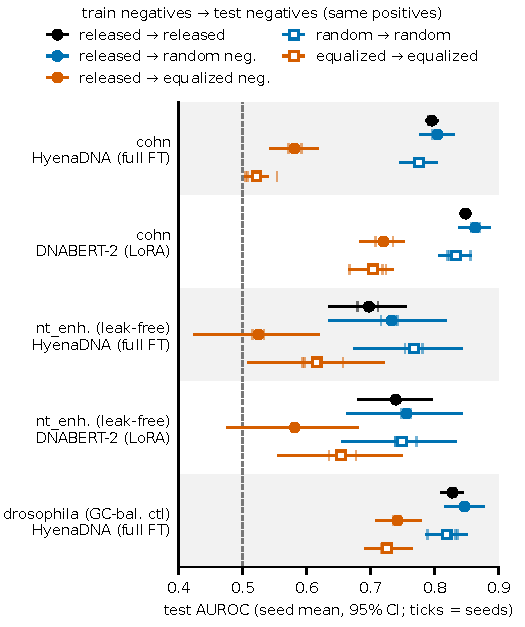
\includegraphics[width=0.52\linewidth]{figs/fm_finetune_v2.pdf}
\caption{Fine-tuned models: test AUROC by training arm $\to$ test negatives (seed mean, 95\% CI;
ticks: individual seeds; in-figure ``released'' denotes the original benchmark negatives). The HyenaDNA \task{cohn} equalized$\to$equalized point is a degenerate
one-class fit (all three seeds) and is not evidence that the arm is unlearnable. \task{nt\_enh.} is on
its leak-free test. Source: \src{results/upgrades/figures/fm\_finetune\_v2.pdf}.}
\label{fig:ftarms}
\end{figure}

% =====================================================================
\section{Homology re-clustering}\label{sec:s6}

All 15 tasks were re-clustered with MMseqs2~\cite{steinegger2017}: an all-vs-all nucleotide search on
both strands, edges at $\ge$80\% identity (id80, primary; id50, strict) over $\ge$80\% of both
sequences, and connected components as clusters, so near-duplicates chained through intermediates
cannot straddle a split. Two protocols re-score every baseline, each against a control: a purge that
scores the same trained model on the test split minus every test sequence with a training homolog,
against 1000 random removals with the same per-class counts; and a cluster-aware re-split, against a
random re-split, over three split seeds.

A median \smHomMedian\ of test sequences have an id80 training homolog (maximum \smHomMax;
\task{cohn} \smHomCohn). Against the random-removal null, the pre-specified test flags inflation in
\smHomNflag\ of the \smHomNeval\ evaluable tasks; the effect exceeds 0.05 MCC (a post hoc cut) in
\smHomNbig, one of which (\task{nt\_enhancers}) coincides with removing all \smNtDup\ verbatim strong
enhancers (Table~\ref{tab:homtasks}; Fig.~\ref{fig:hom}).

\emph{Labels} (Table~\ref{tab:homlabels}). The purge preserves every label it can score on the
prevalence-adjusted MCC (the purged test set re-weighted so that each class has its original test
proportion; post hoc), because purging can change the class mix, which by itself moves MCC;
\task{human\_nontata\_promoters} passes only after that adjustment (raw purged MCC \smHomNontataRaw,
adjusted \smHomNontataStd). Under cluster-aware re-splits \smHomLabelsSFortyTwo\
labels are unchanged at seed 42 and \smHomLabelsMean\ by split-seed mean.
\task{human\_nontata\_promoters} relabels because of homology (MCC \smHomNontataCl\ against
\smHomNontataRa\ on random re-splits), and the two NT enhancer tasks become solved under random
re-splits too, a re-pooling effect of their separately built test split. The label counts are partly
true by construction (composition labels are task types; once a task fails its contamination vs.\
shared-motif label is set by the model-free gate; the purge re-scores only the MCC and that gate), so
the informative labels are the solved and positional ones.

\emph{Routes.} Route~1 under homology control is in Section~\ref{sec:s2}. Route~2 persists: the splice
rescue is \smHcSplice\ on homology-clean data against \smHcSpliceOrig\ on the same training arm, graded
in bin resolution (Table~\ref{tab:homroutes}). For Route~3, TATA-flag cleaning of homology-clean
\task{cohn} moves the TATA AUROC to \smHcTataFlag\ against \smHcTataPlacebo\ for a size-matched
placebo, composition equalization stays below its size-matched placebo ($k$-mer AUROC \smHcEqK\
against \smHcEqPlacebo\ in one draw; \smHcEqDrawRange\ over \smHcEqDraws\ equally valid matching draws,
median \smHcEqDrawMed), the control-motif panel and the TSS depletion are preserved, and the \task{cohn}
FM shortcut persists (frozen probes; fine-tuned HyenaDNA). On homology-clean \task{nt\_enhancers} the frozen probes
shrink but every CI still excludes 0, while the fine-tuned GC-matched shortcut vanishes
(Table~\ref{tab:ftposthoc}).

\emph{Limits.} MMseqs2 cannot seed very short or mostly-N sequences: \smMissedEnh\ short exact twins in
\task{human\_enhancers\_ensembl} (median \smMissedEnhLen\ bp) and \smMissedWorm\ masked all-N sequences in
\task{demo\_human\_or\_worm} are reported as a sensitivity analysis, not merged into the graph.
Many tests are uncorrected for multiplicity; the pre-specified rules and the named primary Route-1 test
are the calls. The semi-synthetic dose-response is not re-run, by design (its random backgrounds have
no natural homology), and DNABERT-2 fine-tuning on the homology-clean splits was not run
(Section~\ref{sec:s9}).

% generated by bibm/supplement/make_sm_tables.py -- do not edit; sources: homology_recluster_table.csv, homology_recluster_paper_table.csv
\begin{table}[!htbp]
\caption{Homology re-clustering (MMseqs2, id80): train/test homology, purge vs.\ random-removal null, and cluster-aware vs.\ random re-splits for all 15 tasks. Source: \src{homology\_recluster\_table.csv},\enspace \src{homology\_recluster\_paper\_table.csv}.}
\label{tab:homtasks}
\centering
\scriptsize
\setlength{\tabcolsep}{2pt}
\begin{tabular}{lrrrlllllr}
\toprule
 & \multicolumn{2}{c}{Test sequences} &  & \multicolumn{3}{c}{Purge vs.\ random removal} & \multicolumn{3}{c}{Re-split (seeds 42--44)} \\
Task & homolog & exact dup. & MCC & MCC raw/adj. & effect ($p$) & flag & cluster/random & cl.$-$rand.\ [range] & robust \\
\midrule
\task{human\_or\_worm} & 11.2\% & 2.6\% & 0.914 & 0.908 / 0.908 & −0.006 ($<$0.001) & yes & 0.909 / 0.912 & −0.003 [−0.009, +0.001] & no \\
\task{regulatory} & 6.1\% & 0.0\% & 0.907 & 0.905 / 0.906 & −0.001 (0.030) & no & 0.911 / 0.911 & 0.000 [−0.000, +0.001] & no \\
\task{nt\_prom\_all} & 3.9\% & 0.4\% & 0.888 & 0.888 / 0.887 & −0.001 (0.33) & no & 0.888 / 0.883 & +0.006 [+0.002, +0.010] & no \\
\task{nt\_prom\_no\_tata} & 3.7\% & 0.3\% & 0.887 & 0.885 / 0.885 & −0.002 (0.090) & no & 0.881 / 0.886 & −0.005 [−0.008, +0.000] & no \\
\task{nontata} & 44.9\% & 0.0\% & 0.874 & 0.469 / 0.768 & −0.058 ($<$0.001) & yes & 0.638 / 0.869 & −0.231 [−0.243, −0.211] & yes \\
\task{nt\_prom\_tata} & 4.7\% & 1.0\% & 0.846 & 0.842 / 0.840 & −0.006 (0.20) & no & 0.883 / 0.869 & +0.013 [−0.008, +0.040] & no \\
\task{coding} & 18.8\% & 0.1\% & 0.800 & 0.777 / 0.777 & −0.023 ($<$0.001) & yes & 0.706 / 0.801 & −0.095 [−0.137, −0.023] & yes \\
\task{enh\_ensembl} & 42.9\% & 38.0\% & 0.593 & 0.427 / 0.490 & −0.089 ($<$0.001) & yes & 0.544 / 0.596 & −0.051 [−0.074, −0.037] & yes \\
\task{mouse\_enh} & 0.0\% & 0.0\% & 0.529 & 0.529 / 0.529 & 0.000 (1.0) & no & 0.518 / 0.542 & −0.024 [−0.071, +0.066] & no \\
\task{nt\_enhancers} & 27.0\% & 25.0\% & 0.514 & 0.303 / 0.317 & −0.179 ($<$0.001) & yes & 0.821 / 0.867 & −0.045 [−0.063, −0.027] & no \\
\task{nt\_enh\_types} & 27.0\% & 25.0\% & 0.476 & n/e & n/e & n/e & 0.769 / 0.759 & +0.010 [−0.090, +0.084] & no \\
\task{cohn} & 4.3\% & 0.0\% & 0.461 & 0.449 / 0.450 & −0.012 ($<$0.001) & yes & 0.451 / 0.460 & −0.009 [−0.027, +0.002] & no \\
\task{ocr} & 11.2\% & 0.0\% & 0.421 & 0.400 / 0.400 & −0.021 ($<$0.001) & yes & 0.400 / 0.424 & −0.024 [−0.042, −0.010] & yes \\
control & 2.1\% & 0.0\% & 0.398 & 0.388 / 0.388 & −0.010 ($<$0.001) & yes & 0.366 / 0.365 & +0.001 [−0.014, +0.021] & no \\
\task{splice} & 12.3\% & 7.4\% & 0.244 & 0.184 / 0.180 & −0.063 ($<$0.001) & yes & 0.195 / 0.271 & −0.076 [−0.095, −0.061] & yes \\
\bottomrule
\end{tabular}
\par\smallskip
\begin{minipage}{\linewidth}\footnotesize\raggedright
Test w/ homolog: test sequences whose connected component contains a training sequence (both strands; $\ge$80\% identity over $\ge$80\% of both sequences). Purge: the same trained model scored on the test split minus those sequences; raw and prevalence-adjusted MCC (the purged test set re-weighted so that each class has its original test proportion; post hoc, chosen after the first results). Effect vs.\ null: purged minus the mean of 1000 random removals with the same per-class counts; Flag: the pre-specified homology-inflation call. For \task{nt\_enhancers} the purge removes all 100 verbatim strong enhancers; against a subtype-matched null the effect is −0.008 ($p$ = 0.28). Re-split: mean over split seeds 42--44; seed-robust = the pre-specified seed-42 call (CI below 0) and cluster $<$ random in all three seeds. n/e: a class is eliminated by the purge. The 0.05-MCC materiality cut used in the text is post hoc.
\end{minipage}
\end{table}

% generated by bibm/supplement/make_sm_tables.py -- do not edit; sources: homology_recluster_labels_addendum.csv, homology_recluster_paper_table.csv
\begin{table}[!htbp]
\caption{Route labels after homology control, against the paper's Table~I labels. Source: \src{homology\_recluster\_labels\_addendum.csv},\enspace \src{homology\_recluster\_paper\_table.csv}.}
\label{tab:homlabels}
\centering
\scriptsize
\setlength{\tabcolsep}{2.5pt}
\begin{tabular}{>{\raggedright\arraybackslash}p{0.145\linewidth}>{\raggedright\arraybackslash}p{0.09\linewidth}>{\raggedright\arraybackslash}p{0.12\linewidth}>{\raggedright\arraybackslash}p{0.11\linewidth}>{\raggedright\arraybackslash}p{0.11\linewidth}>{\raggedright\arraybackslash}p{0.09\linewidth}l>{\raggedright\arraybackslash}p{0.15\linewidth}}
\toprule
Task & Table I & Purge (prev.-adj.\ MCC) & Cluster re-split, seed 42 & Cluster re-split, seed mean & Random re-split & MCC cl./rand. & Reading \\
\midrule
\task{human\_or\_worm} & composition & task type (unchanged by construction) & task type (unchanged by construction) & task type (unchanged by construction) & -- & 0.91/0.91 & composition signal preserved \\
\task{regulatory} & solved & solved & solved & solved & solved & 0.91/0.91 &  \\
\task{nt\_prom\_all} & solved & solved & solved & solved & solved & 0.89/0.88 &  \\
\task{nt\_prom\_no\_tata} & solved & solved & solved & solved & solved & 0.88/0.89 &  \\
\task{nontata} & solved & solved & shared-motif & shared-motif & solved & 0.64/0.87 & relabel attributable to homology \\
\task{nt\_prom\_tata} & solved & solved & solved & solved & solved & 0.88/0.87 &  \\
\task{coding} & composition & task type (unchanged by construction) & task type (unchanged by construction) & task type (unchanged by construction) & -- & 0.71/0.80 & composition signal preserved \\
\task{enh\_ensembl} & contamination (weak) & gate fires (preserved) & gate fires (CLI: Route 3) & gate fires (CLI: Route 3) & -- & 0.54/0.60 & rests on the TATA gate alone \\
\task{mouse\_enh} & composition & task type (unchanged by construction) & task type (unchanged by construction) & task type (unchanged by construction) & -- & 0.52/0.54 & composition signal preserved \\
\task{nt\_enhancers} & contamination & contamination & solved & solved & solved & 0.82/0.87 & also under random re-splits (re-pooling) \\
\task{nt\_enh\_types} & shared-motif & n/e & solved & solved & solved & 0.77/0.76 & also under random re-splits (re-pooling) \\
\task{cohn} & contamination & contamination & contamination & contamination & contamination & 0.45/0.46 &  \\
\task{ocr} & shared-motif & shared-motif & shared-motif & shared-motif & shared-motif & 0.40/0.42 &  \\
control & shared-motif & shared-motif & shared-motif & shared-motif & shared-motif & 0.37/0.37 &  \\
\task{splice} & positional & positional & positional & positional & positional & 0.20/0.27 &  \\
\bottomrule
\end{tabular}
\par\smallskip
\begin{minipage}{\linewidth}\footnotesize\raggedright
Unchanged against Table~I: 12/15 at seed 42 and 12/15 by split-seed mean; the purge preserves every label it can score on the prevalence-adjusted MCC (\task{human\_nontata\_promoters} would relabel on the raw purged MCC). These counts are partly true by construction: the composition labels are task types; once a task fails, contamination vs.\ shared-motif is set by the model-free TATA gate; and the purge re-scores only the MCC and that gate. The informative labels are the solved and positional ones. A relabel is attributed to homology only if the random re-split does not reproduce it.
\end{minipage}
\end{table}

% generated by bibm/supplement/make_sm_tables.py -- do not edit; sources: homology_recluster_positional.csv, homology_recluster_extra_graded.csv, homology_recluster_interventions.csv, homology_recluster_extra_cleaning.csv, homology_recluster_e1_draws_summary.csv, homology_recluster_extra_coords.csv, homology_recluster_extra_specificity.csv, homology_recluster_extra_fm.csv
\begin{table}[!htbp]
\caption{Routes 2 and 3 and the frozen FM probe on homology-clean data (cluster-aware re-split plus one representative per component and label). Source: \src{homology\_recluster\_positional.csv},\enspace \src{homology\_recluster\_extra\_graded.csv},\enspace \src{homology\_recluster\_interventions.csv},\enspace \src{homology\_recluster\_extra\_cleaning.csv},\enspace \src{homology\_recluster\_e1\_draws\_summary.csv},\enspace \src{homology\_recluster\_extra\_coords.csv},\enspace \src{homology\_recluster\_extra\_specificity.csv},\enspace \src{homology\_recluster\_extra\_fm.csv}.}
\label{tab:homroutes}
\centering
\scriptsize
\setlength{\tabcolsep}{3pt}
\begin{tabular}{l>{\raggedright\arraybackslash}p{0.5\linewidth}>{\raggedright\arraybackslash}p{0.33\linewidth}}
\toprule
Route & Readout & Value \\
\midrule
Route 2 & splice $\Delta$MCC ($B{=}8{-}B{=}1$), original (20,001-sequence training arm) & +0.601 [+0.571, +0.629] \\
Route 2 & splice $\Delta$MCC ($B{=}8{-}B{=}1$), homology-clean id80 & +0.620 [+0.590, +0.651] \\
Route 2 & splice $\Delta$MCC ($B{=}8{-}B{=}1$), homology-clean id50 & +0.653 [+0.621, +0.684] \\
Route 2 & splice, graded over $B\in\{2,4,8,16\}$ (id80) & +0.476, +0.549, +0.620, +0.672 \\
Route 2 & selectivity (pre-specified: CI includes 0 or $|\Delta|\le$0.05) on the non-positional tasks (id80) & 12/13 pass \\
Route 2 & selectivity violation: \task{nontata} (id80; a loss, not a rescue) & −0.092 [−0.125, −0.056] \\
Route 3 & \task{cohn} TATA motif-only / GC-content AUROC, original $\to$ equalized (id80) & 0.370$\to$0.500; 0.738$\to$0.506 \\
Route 3 & \task{cohn} TATA-flag cleaning vs.\ size-matched placebo (id80): TATA AUROC; $k$-mer MCC & 0.435 vs.\ 0.373 (uncleaned 0.370); 0.395 vs.\ 0.428 \\
Route 3 & \task{nt\_enhancers} TATA-flag cleaning vs.\ size-matched placebo (id80): TATA AUROC; $k$-mer MCC & 0.486 vs.\ 0.389 (uncleaned 0.390); 0.833 vs.\ 0.882 \\
Route 3 & \task{cohn} equalization vs.\ size-matched placebo (id80; one draw, X1): $k$-mer AUROC & 0.625 [0.582, 0.666] vs.\ 0.737 [0.700, 0.772]; 20 draws 0.551--0.633 (median 0.606) \\
Route 3 & \task{cohn} TATA-flagged negatives at a TSS vs.\ unflagged (id80) & 1.9\% vs.\ 3.5\% ($\times$0.55; Fisher $p$ = 3.1{\texttimes}10\textsuperscript{−8}) \\
Route 3 & control-motif panel, \task{cohn} (id80) & real TATA 0.377; scrambled TBP panel 0.377; random IC panel 0.504 \\
Route 3 & control-motif panel, \task{nt\_enhancers} (id80) & real TATA 0.388; scrambled TBP panel 0.392; random IC panel 0.508 \\
FM probe & frozen HyenaDNA [SEP], \task{cohn}: test effect (id80) & −0.051 [−0.056, −0.046] \\
FM probe & frozen HyenaDNA [SEP], \task{nt\_enhancers}: test effect (id80) & −0.063 [−0.100, −0.030] \\
FM probe & frozen DNABERT-2 mean, \task{cohn}: test effect (id80) & −0.043 [−0.048, −0.039] \\
FM probe & frozen DNABERT-2 mean, \task{nt\_enhancers}: test effect (id80) & −0.019 [−0.033, −0.008] \\
\bottomrule
\end{tabular}
\par\smallskip
\begin{minipage}{\linewidth}\footnotesize\raggedright
Equalized-arm TATA and GC-content AUROCs are partly true by construction, so the cleaning-vs.-placebo rows are the less circular replication; their $k$-mer MCC compares cleaning with removing as many negatives at random. The equalized $k$-mer AUROC depends on the matching draw: its row shows one draw (X1; equalized TATA AUROC 0.492; the TATA/GC-content row uses another, E1) and the range over 20 equally valid draws, all below the placebo's CI. The homology-clean \task{nt\_enhancers} equalized arm keeps 3 test negatives at id80 (1 at id50; MCC not evaluable). GC-content AUROC: the AUROC of per-sequence GC content.
\end{minipage}
\end{table}


\begin{figure}[!htbp]
\centering
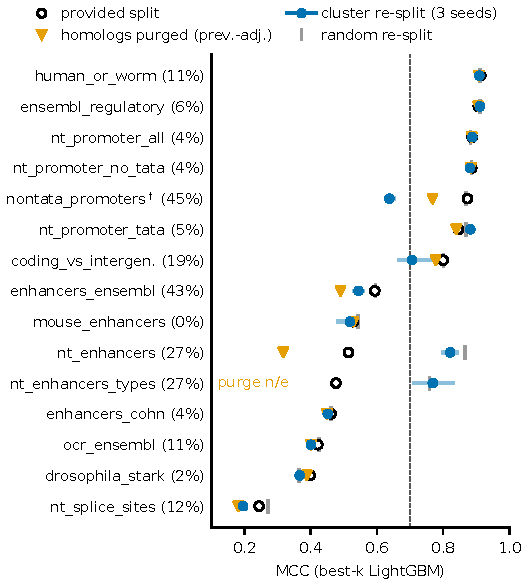
\includegraphics[width=0.55\linewidth]{figs/homology_recluster_mcc.pdf}
\caption{MCC of the best-$k$ LightGBM per task under homology control: provided split (open circle),
test purged of training homologs (triangle; prevalence-adjusted MCC; raw purged MCC of
\task{human\_nontata\_promoters} \smHomNontataRaw), cluster-aware re-split (filled; mean and range over
split seeds 42--44) and random re-split (bar). Percent: test sequences with an id80 training homolog.
Dashed line: the 0.7 ``solved'' threshold. The \task{nt\_enhancers} purge removes all \smNtDup\ verbatim
strong enhancers; the NT-enhancer tasks rise under random re-splits as well (re-pooling). Purge n/e: a
class is eliminated. Source: \src{results/upgrades/figures/homology\_recluster\_mcc.pdf}.}
\label{fig:hom}
\end{figure}

% =====================================================================
\section{Alternative interpretable classifiers}\label{sec:s7}

$k$-mer spectra map onto transcription-factor motifs and are the established interpretable
representation for regulatory sequence~\cite{lee2011,ghandi2014}; gradient-boosted trees capture
non-linear $k$-mer effects on a CPU and expose the per-feature split gains that the paper's motif
enrichment uses. To test whether the diagnosis depends on this classifier, every model-dependent
diagnostic was refit with MCC-tuned L1/L2 logistic regression (LR; penalty and $C$ chosen by validation MCC)
and an explainable boosting machine (EBM)~\cite{lou2013} on the 20-dimensional composition signature
plus the 128 $k$-mers with the largest training-only ANOVA $F$. Only the classifier varies; the
representation is the same $k$-mer spectrum. Model-free diagnostics (motif-only AUROCs, the TATA
gate, the GC-content AUROC, coordinates, the control-motif panel) do not depend on the classifier and were not
recomputed.

Against the paper's Table~I labels, LR and the EBM each keep \smAltSame\ labels and \smAltFailKept\
failure-route labels (Tables~\ref{tab:altagree} and~\ref{tab:altlabels}). The counts are partly true by
construction; the informative checks are the solved and positional labels, and each change is a
solved task that the weaker model fails (regulatory under LR; \task{human\_nontata\_promoters} under
the 128-$k$-mer EBM, solved again with 512 $k$-mers). Splice is the only positional task under every
model, and the dose-response slope persists, but the real-task correlation is not significant under
LR or the EBM (Table~\ref{tab:altroutes}).

No model-level Route-3 readout is contamination-specific (Tables~\ref{tab:altroute3}
and~\ref{tab:altretrained}). Every task tested loses some AUROC beyond size-matched random negatives,
the control included. Under overlap weighting \task{cohn} loses a larger share than the control under
every model, but for LightGBM the composition-only baseline shows the same contrast, and under the EBM,
which sees composition explicitly, the solved gate-positive \task{human\_nontata\_promoters} also loses
more than the control. The weak-excess gate-positive \task{human\_enhancers\_ensembl} also loses AUROC
beyond random negatives, but under overlap weighting a smaller share than the control with LightGBM and
LR (with the EBM the CI of the difference includes 0); its label rests on the TATA gate alone (Table~\ref{tab:homlabels}). Retrained against random negatives, the \task{cohn}-minus-control difference is
significant only for the MCC-tuned LR (\smRetrR; AUROC-tuned LR \smRetrA; LightGBM \smRetrL; EBM
\smRetrE). The overlap shares of \task{nt\_enhancers} exceed 1 and are not interpretable. Motif
attributions agree only partly across classifiers (Table~\ref{tab:altattr}). Only the classifier was
varied: no gapped-$k$-mer SVM or other representation was run in this analysis.

% generated by bibm/supplement/make_sm_tables.py -- do not edit; sources: alt_model_agreement.csv
\begin{table}[!htbp]
\caption{Route labels under alternative interpretable classifiers, against the paper's Table~I labels (post hoc mapping). Source: \src{alt\_model\_agreement.csv}.}
\label{tab:altagree}
\centering
\footnotesize
\begin{tabular}{llll}
\toprule
Classifier & Same label & Failure-route labels kept & Changes (task: new label) \\
\midrule
LightGBM & 15/15 & 7/7 & none \\
LR (MCC-tuned L1/L2) & 14/15 & 7/7 & human\_ensembl\_regulatory:shared-motif \\
EBM (128 $k$-mers) & 14/15 & 7/7 & human\_nontata\_promoters:contamination (weak) \\
EBM (512 $k$-mers) & 15/15 & 7/7 & none \\
\bottomrule
\end{tabular}
\par\smallskip
\begin{minipage}{\linewidth}\footnotesize\raggedright
Only the classifier is varied; the representation stays the $k$-mer spectrum at LightGBM's validation-selected $k$ (the EBM sees the 20-d composition signature plus a train-selected $k$-mer subset). The counts are partly true by construction: composition labels are task types, and once a task fails its contamination vs.\ shared-motif label is set by the model-free TATA gate, so a weaker model can hardly change a failure label. The informative checks are the solved and positional labels: each change is a solved task that the weaker model fails.
\end{minipage}
\end{table}

% generated by bibm/supplement/make_sm_tables.py -- do not edit; sources: alt_model_labels.csv
\begin{table}[!htbp]
\caption{Per-task labels (MCC) under each classifier, mapped to the paper's Table~I vocabulary. Source: \src{alt\_model\_labels.csv}.}
\label{tab:altlabels}
\centering
\scriptsize
\setlength{\tabcolsep}{2pt}
\begin{tabular}{llllll}
\toprule
Task & Table I & LightGBM & LR & EBM-128 & EBM-512 \\
\midrule
\task{human\_or\_worm} & composition & composition (0.911) & composition (0.904) & composition (0.902) & composition (0.914) \\
\task{regulatory} & solved & solved (0.899) & \textbf{shared-motif} (0.389) & solved (0.879) & solved (0.879) \\
\task{nt\_prom\_all} & solved & solved (0.886) & solved (0.821) & solved (0.881) & solved (0.887) \\
\task{nt\_prom\_no\_tata} & solved & solved (0.887) & solved (0.814) & solved (0.876) & solved (0.889) \\
\task{nontata} & solved & solved (0.874) & solved (0.782) & \textbf{contam. (weak)} (0.673) & solved (0.717) \\
\task{nt\_prom\_tata} & solved & solved (0.846) & solved (0.836) & solved (0.894) & solved (0.898) \\
\task{coding} & composition & composition (0.800) & composition (0.789) & composition (0.737) & composition (0.785) \\
\task{enh\_ensembl} & contam. (weak) & contam. (weak) (0.569) & contam. (weak) (0.570) & contam. (weak) (0.481) & contam. (weak) (0.498) \\
\task{mouse\_enh} & composition & composition (0.529) & composition (0.488) & composition (0.554) & composition (0.546) \\
\task{nt\_enhancers} & contamination & contamination (0.514) & contamination (0.421) & contamination (0.449) & contamination (0.473) \\
\task{nt\_enh\_types} & shared-motif & shared-motif (0.476) & shared-motif (0.347) & shared-motif (0.348) & shared-motif (0.428) \\
\task{cohn} & contamination & contamination (0.461) & contamination (0.453) & contamination (0.423) & contamination (0.443) \\
\task{ocr} & shared-motif & shared-motif (0.399) & shared-motif (0.386) & shared-motif (0.349) & shared-motif (0.366) \\
control & shared-motif & shared-motif (0.398) & shared-motif (0.376) & shared-motif (0.372) & shared-motif (0.385) \\
\task{splice} & positional & positional (0.243) & positional (0.203) & positional (0.229) & positional (0.249) \\
\bottomrule
\end{tabular}
\par\smallskip
\begin{minipage}{\linewidth}\footnotesize\raggedright
Bold: a label that differs from Table~I. MCC on the pre-specified capped training arm (tasks capped at 50k training sequences); uncapped refits change no label.
\end{minipage}
\end{table}

% generated by bibm/supplement/make_sm_tables.py -- do not edit; sources: alt_model_route2.csv, alt_model_dose.csv, alt_model_route1.csv
\begin{table}[!htbp]
\caption{Routes 1 and 2 under each classifier. Source: \src{alt\_model\_route2.csv},\enspace \src{alt\_model\_dose.csv},\enspace \src{alt\_model\_route1.csv}.}
\label{tab:altroutes}
\centering
\scriptsize
\setlength{\tabcolsep}{3pt}
\begin{tabular}{lllllll}
\toprule
Classifier & Splice $\Delta$MCC ($B{=}8{-}1$) & Largest other $|\Delta|$ & Dose slope (pooled) & Real-task $\rho$, $n{=}11$ & Real-task $\rho$, $n{=}9^\dagger$ & Presence $\rho$ (GB, $n{=}9$) \\
\midrule
LightGBM & +0.601 [+0.571, +0.629] & 0.028 & +1.99 [+1.92, +2.06] & +0.74 ($p$ 0.013) & +0.87 ($p$ 0.0045) & −0.03 \\
LR (MCC-tuned L1/L2) & +0.681 [+0.654, +0.711] & 0.035 & +1.95 [+1.88, +2.01] & +0.27 ($p$ 0.42) & +0.13 ($p$ 0.74) & −0.15 \\
EBM (128 $k$-mers) & +0.440 [+0.409, +0.470] & 0.031 & +1.81 [+1.73, +1.87] & +0.47 ($p$ 0.14) & +0.47 ($p$ 0.21) & −0.27 \\
\bottomrule
\end{tabular}
\par\smallskip
\begin{minipage}{\linewidth}\footnotesize\raggedright
Splice rescue on the same 20{,}001-sequence training arm for every model; the EBM with position-binned $k$-mers guaranteed (post hoc) gives +0.450. Largest other $|\Delta|$: largest CI-significant change on the other tasks. Dose slope: semi-synthetic dose-response, 135 settings. Real-task $\rho$: uncapped MCCs where available (the EBM keeps its capped MCC on the regulatory task). $^\dagger$ Without \task{human\_nontata\_promoters} and \task{nt\_enhancers}. Presence: Spearman of MCC with the number of enriched TFs.
\end{minipage}
\end{table}

% generated by bibm/supplement/make_sm_tables.py -- do not edit; sources: alt_model_route3_sizecontrolled.csv, alt_model_route3_overlap_contrast.csv, psm_sensitivity_between_dataset.csv
\begin{table}[!htbp]
\caption{Route-3 model-level readouts under each classifier (post hoc). Source: \src{alt\_model\_route3\_sizecontrolled.csv},\enspace \src{alt\_model\_route3\_overlap\_contrast.csv},\enspace \src{psm\_sensitivity\_between\_dataset.csv}.}
\label{tab:altroute3}
\centering
\footnotesize
\begin{tabular}{llll}
\toprule
Task & LightGBM & LR (MCC-tuned L1/L2) & EBM (128 $k$-mers) \\
\midrule
\multicolumn{4}{@{}l}{\emph{AUROC loss beyond size-matched random negatives (random $-$ matched)}} \\
\task{cohn} & +0.152 [+0.110, +0.193] & +0.170 [+0.124, +0.212] & +0.132 [+0.091, +0.172] \\
\task{nt\_enhancers} (leak-free test) & +0.087 [−0.035, +0.217] & +0.062 [−0.045, +0.167] & +0.093 [−0.034, +0.225] \\
control & +0.101 [+0.063, +0.142] & +0.090 [+0.047, +0.133] & +0.108 [+0.065, +0.149] \\
\task{enh\_ensembl} & +0.026 [+0.018, +0.034] & +0.050 [+0.041, +0.059] & +0.037 [+0.027, +0.047] \\
\task{ocr} & +0.036 [+0.027, +0.046] & +0.045 [+0.036, +0.054] & +0.045 [+0.035, +0.054] \\
\multicolumn{4}{@{}l}{\emph{Overlap weighting, model fixed: share of above-chance AUROC lost, task $-$ GC-balanced control}} \\
\task{cohn} & +0.353 [+0.293, +0.413] & +0.292 [+0.228, +0.353] & +0.419 [+0.350, +0.487] \\
\task{nt\_enhancers} & not interpretable & not interpretable & not interpretable \\
\task{enh\_ensembl} & −0.122 [−0.169, −0.079] & −0.137 [−0.195, −0.087] & −0.047 [−0.103, +0.004] \\
\task{ocr} & −0.112 [−0.158, −0.068] & −0.138 [−0.195, −0.088] & −0.074 [−0.132, −0.022] \\
\task{nontata} & −0.229 [−0.276, −0.187] & −0.090 [−0.150, −0.037] & +0.201 [+0.134, +0.260] \\
\bottomrule
\end{tabular}
\par\smallskip
\begin{minipage}{\linewidth}\footnotesize\raggedright
Loss beyond random: random-negative AUROC minus AUROC on the released equalized split. Every task tested loses some AUROC beyond random negatives, the GC-balanced control included. Overlap contrast: share of above-chance AUROC the unretrained model loses under overlap weighting, task minus control; for \task{nt\_enhancers} the weights over-correct (weighted AUROC below 0.5, share above 1), so its share is not interpretable. The LightGBM contrast for \task{cohn} is matched by the composition-only model's contrast under the same weights (+0.352; Table~\ref{tab:psmbetween}), so these contrasts measure reliance on the composition gap, not contamination specificity. Under the EBM, which sees composition explicitly, the solved gate-positive \task{human\_nontata\_promoters} also loses more than the control.
\end{minipage}
\end{table}

% generated by bibm/supplement/make_sm_tables.py -- do not edit; sources: alt_model_route3_contrast.csv
\begin{table}[!htbp]
\caption{Retrained random-negative design: share of above-chance AUROC lost, \task{cohn} minus the GC-balanced control (post hoc). Source: \src{alt\_model\_route3\_contrast.csv}.}
\label{tab:altretrained}
\centering
\footnotesize
\begin{tabular}{llll}
\toprule
Classifier & \task{cohn} & Control & Difference [CI] \\
\midrule
LightGBM & 0.573 & 0.386 & +0.187 [−0.014, +0.390] \\
LR (MCC-tuned L1/L2) & 0.662 & 0.358 & +0.305 [+0.091, +0.529] \\
LR (AUROC-tuned) & 0.563 & 0.392 & +0.171 [−0.038, +0.390] \\
EBM (128 $k$-mers) & 0.500 & 0.427 & +0.074 [−0.128, +0.289] \\
\bottomrule
\end{tabular}
\par\smallskip
\begin{minipage}{\linewidth}\footnotesize\raggedright
The difference excludes 0 only for the MCC-tuned LR; with the AUROC-tuned LR it does not. No model-level readout here is contamination-specific.
\end{minipage}
\end{table}

% generated by bibm/supplement/make_sm_tables.py -- do not edit; sources: alt_model_attribution.csv
\begin{table}[!htbp]
\caption{Motif attribution under each classifier (post hoc): the paper's named TFs on \task{human\_nontata\_promoters}, and agreement with LightGBM across tasks. Source: \src{alt\_model\_attribution.csv}.}
\label{tab:altattr}
\centering
\footnotesize
\begin{tabular}{llllll}
\toprule
Classifier & SP1 rank & SP2 rank & Jaccard vs.\ LightGBM (nontata) & Median Jaccard (all tasks) & Median $z$-profile $\rho$ \\
\midrule
LightGBM & 1 & 2 & -- & -- & -- \\
LR (MCC-tuned L1/L2) & 6 & 4 & 0.49 & 0.25 & 0.76 \\
EBM (128 $k$-mers) & 4 & 8 & 0.55 & 0.37 & 0.83 \\
\bottomrule
\end{tabular}
\par\smallskip
\begin{minipage}{\linewidth}\footnotesize\raggedright
Ranks among FDR-enriched vertebrate JASPAR TFs by importance-weighted enrichment; Jaccard: overlap of enriched TF sets.
\end{minipage}
\end{table}


% =====================================================================
\section{The GUE suite}\label{sec:s8}

The unchanged pipeline and route thresholds were applied to the 28 datasets of GUE~\cite{dnabert2}
(human, mouse, yeast and virus), with predictions stated before the run (Table~\ref{tab:guepred}). GUE
is separately assembled but mostly not new DNA (Table~\ref{tab:guefam}): only \smGueNear\ of the 28
datasets are near-disjoint from GB/NT (at most \smNearMax\ of sequences shared; only covid shares none),
\smGueHumanTF\ of the human-TF sequences occur in GB/NT, and the promoter positives, most splice
sequences and all yeast sequences are NT data.

The rule gives \smGueFail\ failure routes (\smGuePos\ positional, \smGueShared\ shared-motif,
\smGueContam\ contamination), \smGueSolved\ solved and \smGueHard\ ``hard'' labels (MCC below 0.7 with no
single route; Table~\ref{tab:gue}).
Every failure route falls on a dataset that shares at least \smGueMinShared\ of its sequences with
GB/NT. The positional rule fires on splice ($\Delta$MCC \smGueDeltaSplice) and, against our pre-stated
prediction, also on both TATA-promoter tasks (\smGueDeltaCore\ and \smGueDeltaThreeHundred).
\task{prom\_300\_tata} has the same positives as \task{nt\_promoter\_tata}, yet on \task{nt\_promoter\_tata}
the same code gives \smNtPromTataDelta, not significant: with identical positives, the route follows how
the negatives were built. (The GUE negatives of the two TATA tasks differ from NT's, although
\smPromLabelZero\ of their label-0 sequences also occur in the paper's tasks.)

Only the three positional labels survive our post hoc checks. The five yeast shared-motif labels depend
on a length-dependent richness threshold (Table~\ref{tab:guerule}), which also makes \smGueHardRich\ short tasks
``hard''. The four yeast contamination labels fall on measured low-signal genomic windows (the
low-signal class of each histone-mark dataset), not on sampled negatives, and genomic location accounts
for only \smEmpShareLo--\smEmpShareHi\ of their TATA excess with two location strata
(Table~\ref{tab:gueemp}); they are not evidence of negative-set contamination. Of the
\smGuePredApplicable\ applicable pre-stated predictions, \smGuePredFail\ failed. A split artifact outside
the three routes appears in the mouse-TF tasks, whose dinucleotide-shuffle negatives were split
independently of their source positives: the composition-only baseline inverts (AUROC \smTwinAuc;
Table~\ref{tab:guetwins}). When negatives are shuffles of the positives, each positive and its shuffle
belong in the same split.

On the development tasks the same driver reproduces \smPaperMCCRepro\ of the paper's 15 MCCs, and its rule reproduces
\smCliAgree\ Table~I routes that it can emit (in-sample consistency, not calibration). The CPU $k$-mer
baseline sits a median of \smGueGapMedian\ MCC points (MCC$\times$100) below DNABERT-2 as published, over
the \smGueGapN\ MCC datasets; the comparison only locates the baseline. GUE was difficulty-filtered by its authors, so its
route distribution is not representative of benchmarks in general.

% generated by bibm/supplement/make_sm_tables.py -- do not edit; sources: gue_family_summary.csv
\begin{table}[!htbp]
\caption{GUE task families: how the negatives were built, how much of the DNA is shared with GB/NT, and the labels. Source: \src{gue\_family\_summary.csv}.}
\label{tab:guefam}
\centering
\scriptsize
\setlength{\tabcolsep}{3pt}
\begin{tabular}{>{\raggedright\arraybackslash}p{0.13\linewidth}r>{\raggedright\arraybackslash}p{0.33\linewidth}l>{\raggedright\arraybackslash}p{0.17\linewidth}rr}
\toprule
Family & $n$ & Negatives / label-0 class (as documented) & Shared & Labels & $k$-mer & DNABERT-2 \\
\midrule
Core promoter (70 bp) & 3 & as prom\_300, center -34..+35 bp around the TSS & 50.1--77.4\% & hard:2, positional:1 & 58.2 & 70.5 \\
Promoter (300 bp) & 3 & non-TATA: randomly substituted promoter sequences; TATA: random non-promoter genomic sequences carrying a TATA motif & 50.0--65.8\% & solved:2, positional:1 & 66.8 & 84.2 \\
TF binding, human & 5 & non-overlapping genomic sequences of the same length and GC content (GC-matched) & 19.8--44.8\% & hard:3, solved:2 & 63.1 & 70.1 \\
Splice site (3-class) & 1 & Wang et al. 2019 donor/acceptor/non-site, reconstructed with adversarial negatives & 68.4--68.4\% & positional:1 & 34.7 & 85.0 \\
TF binding, mouse & 5 & dinucleotide-shuffled positives (dinucleotide frequencies preserved) & 0.0--0.2\% & hard:3, solved:2 & 63.5 & 68.0 \\
Yeast histone marks & 10 & Pham et al. 2005 datasets (jaist.ac.jp/\textasciitilde{}tran/nucleosome): yeast genomic windows (ORF and intergenic ChIP-chip regions) with high (label 1) vs low (label 0) relative histone occupancy/modification; no sampled negatives; GUE split 8:1:1 & 100.0--100.0\% & shared-motif:5, contamination:4, solved:1 & 51.5 & 56.0 \\
Covid variant (9-class) & 1 & 9 SARS-CoV-2 variants (GISAID), 1 kb segments & 0.0--0.0\% & solved:1 & 76.8 & 71.0 \\
\bottomrule
\end{tabular}
\par\smallskip
\begin{minipage}{\linewidth}\footnotesize\raggedright
Shared: range over the family's datasets of the fraction of sequences found in GB/NT. Labels: `hard' = MCC below 0.7 with no single route (Table~\ref{tab:gue}). $k$-mer and DNABERT-2: mean MCC$\times$100 (covid: macro-F1$\times$100) of this pipeline's $k$-mer LightGBM and of DNABERT-2 as published; the comparison only locates the baseline. The yeast `negatives' are the measured low-signal class of each mark, not a sampled negative set.
\end{minipage}
\end{table}

% generated by bibm/supplement/make_sm_tables.py -- do not edit; sources: gue_results.csv, gue_overlap_summary.csv, gue_failure_route_audit.csv
\begin{table}[!htbp]
\caption{The 28 GUE datasets under the unchanged pipeline and route thresholds. Source: \src{gue\_results.csv},\enspace \src{gue\_overlap\_summary.csv},\enspace \src{gue\_failure\_route\_audit.csv}.}
\label{tab:gue}
\centering
\scriptsize
\setlength{\tabcolsep}{3pt}
\begin{tabular}{lrllllp{0.2\linewidth}}
\toprule
Dataset & Shared with GB/NT & Class & MCC [CI] & Route & Positional $\Delta$MCC [CI] & Post hoc status \\
\midrule
prom\_core\_all & 52.9\% & shares with the 15 & 0.612 [0.594, 0.632] & hard & +0.019 [+0.005, +0.033] & hard only via richness threshold \\
prom\_core\_notata & 50.1\% & shares with the 15 & 0.646 [0.626, 0.667] & hard & 0.000 [−0.013, +0.014] & hard only via richness threshold \\
prom\_core\_tata & 77.4\% & shares with the 15 & 0.488 [0.412, 0.550] & positional & +0.231 [+0.170, +0.297] & unaffected \\
prom\_300\_all & 51.6\% & shares with the 15 & 0.765 [0.750, 0.781] & solved & +0.037 [+0.025, +0.049] &  \\
prom\_300\_notata & 50.0\% & shares with the 15 & 0.867 [0.854, 0.880] & solved & +0.003 [−0.005, +0.010] &  \\
prom\_300\_tata & 65.8\% & shares with the 15 & 0.371 [0.296, 0.439] & positional & +0.248 [+0.183, +0.317] & unaffected \\
human\_tf\_0 & 44.8\% & shares with the 15 & 0.648 [0.601, 0.692] & hard & −0.004 [−0.037, +0.025] & hard only via richness threshold \\
human\_tf\_1 & 42.4\% & shares with the 15 & 0.700 [0.657, 0.744] & solved & −0.018 [−0.044, +0.009] &  \\
human\_tf\_2 & 44.4\% & shares with the 15 & 0.567 [0.512, 0.622] & hard & +0.021 [−0.012, +0.054] & hard only via richness threshold \\
human\_tf\_3 & 19.8\% & shares with the 15 & 0.479 [0.425, 0.531] & hard & −0.023 [−0.065, +0.020] & hard only via richness threshold \\
human\_tf\_4 & 38.3\% & shares with the 15 & 0.759 [0.718, 0.796] & solved & +0.004 [−0.020, +0.026] &  \\
splice\_reconstructed & 68.4\% & shares with the 15 & 0.347 [0.326, 0.368] & positional & +0.407 [+0.382, +0.432] & unaffected \\
mouse\_tf\_0 & 0.1\% & near-disjoint & 0.577 [0.520, 0.633] & hard & −0.027 [−0.061, +0.010] & hard only via richness threshold \\
mouse\_tf\_1 & 0.0\% & near-disjoint & 0.768 [0.752, 0.783] & solved & −0.006 [−0.015, +0.003] &  \\
mouse\_tf\_2 & 0.2\% & near-disjoint & 0.783 [0.716, 0.844] & solved & +0.023 [−0.025, +0.070] &  \\
mouse\_tf\_3 & 0.1\% & near-disjoint & 0.674 [0.578, 0.766] & hard & −0.016 [−0.050, +0.012] &  \\
mouse\_tf\_4 & 0.1\% & near-disjoint & 0.373 [0.331, 0.414] & hard & −0.020 [−0.051, +0.011] & hard only via richness threshold \\
emp\_H3 & 100.0\% & other NT tasks only & 0.689 [0.651, 0.726] & contamination & +0.005 [−0.018, +0.030] & low-signal windows \\
emp\_H3K14ac & 100.0\% & other NT tasks only & 0.473 [0.442, 0.504] & shared-motif & −0.060 [−0.087, −0.033] & threshold-dependent \\
emp\_H3K36me3 & 100.0\% & other NT tasks only & 0.499 [0.468, 0.527] & contamination & −0.003 [−0.027, +0.018] & low-signal windows \\
emp\_H3K4me1 & 100.0\% & other NT tasks only & 0.414 [0.382, 0.446] & contamination & −0.025 [−0.054, +0.001] & low-signal windows \\
emp\_H3K4me2 & 100.0\% & other NT tasks only & 0.342 [0.309, 0.375] & shared-motif & −0.032 [−0.063, −0.003] & threshold-dependent \\
emp\_H3K4me3 & 100.0\% & other NT tasks only & 0.385 [0.354, 0.415] & shared-motif & −0.079 [−0.110, −0.050] & threshold-dependent \\
emp\_H3K79me3 & 100.0\% & other NT tasks only & 0.627 [0.598, 0.657] & contamination & −0.017 [−0.036, +0.002] & low-signal windows \\
emp\_H3K9ac & 100.0\% & other NT tasks only & 0.535 [0.502, 0.567] & shared-motif & −0.043 [−0.070, −0.017] & threshold-dependent \\
emp\_H4 & 100.0\% & other NT tasks only & 0.723 [0.687, 0.758] & solved & −0.002 [−0.024, +0.018] &  \\
emp\_H4ac & 100.0\% & other NT tasks only & 0.463 [0.432, 0.494] & shared-motif & −0.062 [−0.090, −0.038] & threshold-dependent \\
covid & 0.0\% & near-disjoint & 0.736 [0.727, 0.746] & solved & −0.022 [−0.028, −0.017] &  \\
\bottomrule
\end{tabular}
\par\smallskip
\begin{minipage}{\linewidth}\footnotesize\raggedright
Shared: fraction of the dataset's sequences that occur in GB or NT tasks as exact matches (either strand; containment in either direction). Class: `shares with the 15', shares sequences with the paper's 15 tasks; `other NT tasks only', shares sequences only with NT tasks outside those 15; near-disjoint, at most 0.2\% shared (mouse TF 2--23 sequences per dataset; only covid shares none). Route `hard': MCC below 0.7 and none of the three route rules fires (no single route). Post hoc status of the failure routes: the yeast (EMP) shared-motif labels depend on a length-dependent richness threshold (Table~\ref{tab:guerule}); the yeast contamination labels fall on measured low-signal genomic windows, not sampled negatives (Table~\ref{tab:gueemp}); only the three positional labels are unaffected. Positional deltas other than the three Route-2 tasks are not corrected for multiplicity. covid is 9-class (macro F1 is the GUE metric).
\end{minipage}
\end{table}

% generated by bibm/supplement/make_sm_tables.py -- do not edit; sources: gue_predictions.csv
\begin{table}[!htbp]
\caption{Predictions stated before the GUE run, and their outcomes. Source: \src{gue\_predictions.csv}.}
\label{tab:guepred}
\centering
\scriptsize
\setlength{\tabcolsep}{3pt}
\begin{tabular}{l>{\raggedright\arraybackslash}p{0.36\linewidth}>{\raggedright\arraybackslash}p{0.38\linewidth}l}
\toprule
 & Prediction & Values & Outcome \\
\midrule
P1a & mouse TF (dinucleotide-shuffled negatives): composition-only AUROC within 0.05 of 0.5 & mouse\_tf\_0=0.022, mouse\_tf\_1=0.081, mouse\_tf\_2=0.018, mouse\_tf\_3=0.033, mouse\_tf\_4=0.034 & FAILS \\
P1b & mouse TF: composition fraction \textasciitilde{}0 (read as |fraction| <= 0.10) & mouse\_tf\_0=-1.288, mouse\_tf\_1=-0.914, mouse\_tf\_2=-1.036, mouse\_tf\_3=-1.134, mouse\_tf\_4=-1.784 & FAILS \\
P1c & mouse TF: equalized split retains most (>50\%) negatives & mouse\_tf\_0=0.484, mouse\_tf\_1=0.793, mouse\_tf\_2=0.529, mouse\_tf\_3=0.512, mouse\_tf\_4=0.740 & PARTLY \\
P2 & human TF (GC-matched negatives): GC-content AUROC within 0.05 of 0.5 & human\_tf\_0=0.504, human\_tf\_1=0.511, human\_tf\_2=0.497, human\_tf\_3=0.498, human\_tf\_4=0.503 & HOLDS \\
P3a & splice/reconstructed: significant positive positional delta & delta=+0.4069 [+0.3820,+0.4316] & HOLDS \\
P3b & splice is the only GUE task that can meet the Route-2 rule (significant delta > 0.2) & tasks meeting the delta rule: prom\_core\_tata (+0.231), prom\_300\_tata (+0.248), splice\_reconstructed (+0.407) & FAILS \\
P4 & no magnitude prediction for the promoter tasks & none & not applicable \\
\bottomrule
\end{tabular}
\par\smallskip
\begin{minipage}{\linewidth}\footnotesize\raggedright
Of the 6 applicable predictions (P4 is not applicable), 2 held, 1 held partly and 3 failed: Route~2 is not confined to splice (P3b), and the mouse-TF composition-only baseline is far from chance (P1a, P1b), because shuffle twins were split across train and test (Table~\ref{tab:guetwins}).
\end{minipage}
\end{table}

% generated by bibm/supplement/make_sm_tables.py -- do not edit; sources: gue_rule_sensitivity_summary.csv
\begin{table}[!htbp]
\caption{Route-1 richness threshold normalized by sequence length (post hoc PH4): how many labels change. Source: \src{gue\_rule\_sensitivity\_summary.csv}.}
\label{tab:guerule}
\centering
\scriptsize
\setlength{\tabcolsep}{3pt}
\begin{tabular}{>{\raggedright\arraybackslash}p{0.25\linewidth}rrr>{\raggedright\arraybackslash}p{0.42\linewidth}}
\toprule
Variant & Changed & hard$\to$shared & shared$\to$hard & Label counts / agreement \\
\midrule
as registered & 0 & 0 & 0 & hard (no single route):8; solved:8; shared-motif:5; contamination:4; positional:3 \\
richness per 200 bp & 11 & 6 & 5 & solved:8; hard (no single route):7; shared-motif:6; contamination:4; positional:3 \\
richness per 250 bp & 12 & 7 & 5 & solved:8; shared-motif:7; hard (no single route):6; contamination:4; positional:3 \\
richness per 300 bp (= median paper-15 length) & 11 & 7 & 4 & shared-motif:8; solved:8; hard (no single route):5; contamination:4; positional:3 \\
richness per 400 bp & 7 & 7 & 0 & shared-motif:12; solved:8; contamination:4; positional:3; hard (no single route):1 \\
richness per 500 bp & 7 & 7 & 0 & shared-motif:12; solved:8; contamination:4; positional:3; hard (no single route):1 \\
GB+NT (paper 15): as registered & 0 & 0 & 0 & Table~I agreement 11/12 \\
GB+NT (paper 15): richness per 200 bp & 1 & 0 & 1 & Table~I agreement 10/12 \\
GB+NT (paper 15): richness per 250 bp & 0 & 0 & 0 & Table~I agreement 11/12 \\
GB+NT (paper 15): richness per 300 bp (= median paper-15 length) & 0 & 0 & 0 & Table~I agreement 11/12 \\
GB+NT (paper 15): richness per 400 bp & 0 & 0 & 0 & Table~I agreement 11/12 \\
GB+NT (paper 15): richness per 500 bp & 0 & 0 & 0 & Table~I agreement 11/12 \\
\bottomrule
\end{tabular}
\par\smallskip
\begin{minipage}{\linewidth}\footnotesize\raggedright
The absolute richness threshold is unreachable for the shortest GUE tasks, which is why 7 of the 8 GUE `hard' labels are hard; normalizing it moves labels in both directions only at 200--300 bp. GB/NT lengths lie near the reference length, so their stability is partly mechanical.
\end{minipage}
\end{table}

% generated by bibm/supplement/make_sm_tables.py -- do not edit; sources: gue_emp_provenance.csv
\begin{table}[!htbp]
\caption{Yeast (EMP) datasets with the Route-3 signature: where the label-0 windows come from, and how much of the TATA excess genomic location accounts for (post hoc PH5). Source: \src{gue\_emp\_provenance.csv}.}
\label{tab:gueemp}
\centering
\scriptsize
\setlength{\tabcolsep}{3pt}
\begin{tabular}{llllllrlr}
\toprule
Dataset & Label & Label 1/0 & = Pham & Excess & Location-std.\ (2 strata) [CI] & Accounted & 4 strata & Accounted \\
\midrule
emp\_H3 & contamination & 7{,}667/7{,}298 & yes & +0.270 & +0.175 [+0.147, +0.203] & 35\% & +0.190 & 30\% \\
emp\_H4 & solved & 6{,}480/8{,}121 & yes & +0.332 & +0.198 [+0.160, +0.235] & 40\% & +0.200 & 40\% \\
emp\_H3K4me1 & contamination & 17{,}266/14{,}411 & yes & +0.133 & +0.062 [+0.038, +0.088] & 53\% & +0.078 & 41\% \\
emp\_H3K36me3 & contamination & 18{,}892/15{,}988 & yes & +0.178 & +0.092 [+0.067, +0.118] & 48\% & +0.061 & 65\% \\
emp\_H3K79me3 & contamination & 15{,}337/13{,}500 & yes & +0.262 & +0.172 [+0.144, +0.198] & 34\% & +0.160 & 39\% \\
\bottomrule
\end{tabular}
\par\smallskip
\begin{minipage}{\linewidth}\footnotesize\raggedright
Label counts equal the positive/negative counts of the Pham et al.\ 2005 release on every mark, so label 0 is the measured low-signal class (low modification relative to H3 for the modification marks), not a sampled negative set. Excess: TATA negative-class excess on the uniquely located windows; location-standardized: the same within ORF/intergenic strata (2 strata) or finer strata (4). `Accounted' = share of the excess removed by standardization. With 2 strata the excess falls below the Route-3 threshold (0.10; CI upper bound) for 1 of 5 marks (emp\_H3K4me1); with 4 strata for 0.
\end{minipage}
\end{table}

% generated by bibm/supplement/make_sm_tables.py -- do not edit; sources: gue_twins.csv
\begin{table}[!htbp]
\caption{GUE mouse-TF split artifact: dinucleotide-shuffle negatives were split independently of their source positives (post hoc PH2). Source: \src{gue\_twins.csv}.}
\label{tab:guetwins}
\centering
\footnotesize
\begin{tabular}{lrrrrr}
\toprule
Dataset & Test $n$ & Test w/ cross-label twin in train & Comp.-only AUROC, all & with twin & without twin \\
\midrule
mouse\_tf\_0 & 810 & 81.9\% & 0.023 & 0.000 & 0.520 \\
mouse\_tf\_1 & 6{,}745 & 80.5\% & 0.081 & 0.015 & 0.516 \\
mouse\_tf\_2 & 328 & 81.1\% & 0.018 & 0.000 & 0.493 \\
mouse\_tf\_3 & 239 & 72.8\% & 0.033 & 0.000 & 0.452 \\
mouse\_tf\_4 & 1{,}883 & 80.6\% & 0.034 & 0.000 & 0.458 \\
\bottomrule
\end{tabular}
\par\smallskip
\begin{minipage}{\linewidth}\footnotesize\raggedright
A test sequence whose shuffle twin (same composition, opposite label) is in the training split inverts a composition-only model; on test sequences without such a twin the composition-only AUROC is close to 0.5. When negatives are shuffles of the positives, each positive and its shuffle belong in the same split.
\end{minipage}
\end{table}


% =====================================================================
\section{Analyses packaged but not run (not results)}\label{sec:s9}

Table~\ref{tab:deferred} lists analyses that were packaged or recommended but were not run. None of
them produced a number in the paper or in this supplement; the paper states the corresponding gaps as
limitations (full-parameter fine-tuning covers only the \smFTHParamsM-parameter HyenaDNA-tiny; the GC-balanced
control covers HyenaDNA only; homology-clean fine-tuning covers HyenaDNA only).

% generated by bibm/supplement/make_sm_tables.py -- do not edit; sources: src/upgrades/fm_finetune/gpu_deferred/README.md, src/upgrades/homology_recluster/deferred/README.md, src/upgrades/alt_model/deferred/README.md
\begin{table}[!htbp]
\caption{Analyses packaged or recommended but NOT run. No number in the paper or in this supplement comes from them. Source: \src{src/upgrades/fm\_finetune/gpu\_deferred/README.md},\enspace \src{src/upgrades/homology\_recluster/deferred/README.md},\enspace \src{src/upgrades/alt\_model/deferred/README.md}.}
\label{tab:deferred}
\centering
\footnotesize
\setlength{\tabcolsep}{3pt}
\begin{tabular}{>{\raggedright\arraybackslash}p{0.44\linewidth}>{\raggedright\arraybackslash}p{0.25\linewidth}>{\raggedright\arraybackslash}p{0.25\linewidth}}
\toprule
Analysis (not run) & Why not run & Package / command \\
\midrule
DNABERT-2-117M full-parameter fine-tuning, \task{cohn} and \task{nt\_enhancers} (3 arms $\times$ seeds 42--44; 18 units) & full-model optimizer state exceeds the laptop's GPU memory & \pth{fm_finetune/gpu_deferred/jobs.sh} 2 and 7 \\
NT-v2-500M LoRA fine-tuning, \task{cohn}, \task{nt\_enhancers} and the GC-balanced control (27 units) & 0.5B parameters; days on the laptop & \pth{fm_finetune/gpu_deferred/jobs.sh} 3, 6 and 5 \\
DNABERT-2 LoRA fine-tuning on the homology-clean splits (\task{cohn}, \task{nt\_enhancers}; 18 units) & memory above the per-job budget & \pth{homology_recluster/deferred/run_deferred_dnabert_hc.sh} \\
Uncapped multiclass EBM on \task{human\_ensembl\_regulatory} (1 unit) & about 9--10 h at 3 threads; cannot change a label & \pth{alt_model/deferred/run_ebm_regulatory_full.sh} \\
DNABERT-2 frozen probe and LoRA fine-tuning on the GC-balanced control & not packaged (the exclusion was a choice; Table~\ref{tab:d9}) & -- \\
Seed-pinned re-draw of the dinucleotide-shuffled negatives & not packaged (single-draw dependence is disclosed instead; Table~\ref{tab:shuffle}) & -- \\
\bottomrule
\end{tabular}
\par\smallskip
\begin{minipage}{\linewidth}\footnotesize\raggedright
GPU bundle for the fine-tuning jobs: \pth{external/fm_finetune/gbkb_ft_gpu_bundle.tar.gz}, SHA-256 \task{7e6707d9583c30c7}\ldots (verified). Paths are under \task{src/upgrades/}. After a GPU hand-back, the torch-free scoring chain in \task{src/upgrades/fm\_finetune/README.md} (step 3) re-scores every unit with the same pre-specified rules.
\end{minipage}
\end{table}


\clearpage
\section*{AI-use disclosure}
% TODO(author): confirm this wording; keep it consistent with the paper's AI-use disclosure.
Claude (Anthropic), run as Claude Code agents under the author's direction, wrote the analysis and
table-generating code, ran the analyses, and drafted this supplement. The author designed the study,
inspected and verified the outputs, and takes full responsibility for the content.

\begin{thebibliography}{00}
\bibitem{cohn2018} D. Cohn, O. Zuk, and T. Kaplan, ``Enhancer identification using transfer and
adversarial deep learning of DNA sequences,'' bioRxiv 264200, 2018, doi:10.1101/264200.
\bibitem{liu2016} B. Liu, L. Fang, R. Long, X. Lan, and K.-C. Chou, ``iEnhancer-2L: a two-layer
predictor for identifying enhancers and their strength by pseudo $k$-tuple nucleotide composition,''
\emph{Bioinformatics}, vol.~32, no.~3, pp.~362--369, 2016.
\bibitem{ernst2011} J. Ernst \emph{et al.}, ``Mapping and analysis of chromatin state dynamics in nine
human cell types,'' \emph{Nature}, vol.~473, no.~7345, pp.~43--49, 2011.
\bibitem{liu2018} B. Liu, K. Li, D.-S. Huang, and K.-C. Chou, ``iEnhancer-EL: identifying enhancers and
their strength with ensemble learning approach,'' \emph{Bioinformatics}, vol.~34, no.~22,
pp.~3835--3842, 2018.
\bibitem{geng2022} Q. Geng, R. Yang, and L. Zhang, ``A deep learning framework for enhancer prediction
using word embedding and sequence generation,'' \emph{Biophys. Chem.}, vol.~286, p.~106822, 2022.
\bibitem{costantini2006} M. Costantini, O. Clay, F. Auletta, and G. Bernardi, ``An isochore map of
human chromosomes,'' \emph{Genome Res.}, vol.~16, no.~4, pp.~536--541, 2006.
\bibitem{rosenbaum1983} P. R. Rosenbaum and D. B. Rubin, ``The central role of the propensity score in
observational studies for causal effects,'' \emph{Biometrika}, vol.~70, no.~1, pp.~41--55, 1983.
\bibitem{li2018} F. Li, K. L. Morgan, and A. M. Zaslavsky, ``Balancing covariates via propensity score
weighting,'' \emph{J. Am. Stat. Assoc.}, vol.~113, no.~521, pp.~390--400, 2018.
\bibitem{encode2020} ENCODE Project Consortium \emph{et al.}, ``Expanded encyclopaedias of DNA elements in
the human and mouse genomes,'' \emph{Nature}, vol.~583, no.~7818, pp.~699--710, 2020.
\bibitem{altschul1985} S. F. Altschul and B. W. Erickson, ``Significance of nucleotide sequence
alignments: a method for random sequence permutation that preserves dinucleotide and codon usage,''
\emph{Mol. Biol. Evol.}, vol.~2, no.~6, pp.~526--538, 1985.
\bibitem{hyenadna} E. Nguyen \emph{et al.}, ``HyenaDNA: long-range genomic sequence modeling at single
nucleotide resolution,'' in \emph{Proc. Adv. Neural Inf. Process. Syst. (NeurIPS)}, 2023.
\bibitem{dnabert2} Z. Zhou, Y. Ji, W. Li, P. Dutta, R. Davuluri, and H. Liu, ``DNABERT-2: efficient
foundation model and benchmark for multi-species genomes,'' in \emph{Proc. Int. Conf. Learn. Represent.
(ICLR)}, 2024, arXiv:2306.15006.
\bibitem{hu2022} E. J. Hu \emph{et al.}, ``LoRA: low-rank adaptation of large language models,'' in
\emph{Proc. Int. Conf. Learn. Represent. (ICLR)}, 2022, arXiv:2106.09685.
\bibitem{steinegger2017} M. Steinegger and J. S\"oding, ``MMseqs2 enables sensitive protein sequence
searching for the analysis of massive data sets,'' \emph{Nat. Biotechnol.}, vol.~35, no.~11,
pp.~1026--1028, 2017.
\bibitem{lee2011} D. Lee, R. Karchin, and M. A. Beer, ``Discriminative prediction of mammalian enhancers
from DNA sequence,'' \emph{Genome Res.}, vol.~21, no.~12, pp.~2167--2180, 2011.
\bibitem{ghandi2014} M. Ghandi, D. Lee, M. Mohammad-Noori, and M. A. Beer, ``Enhanced regulatory sequence
prediction using gapped $k$-mer features,'' \emph{PLoS Comput. Biol.}, vol.~10, no.~7, p.~e1003711, 2014.
\bibitem{lou2013} Y. Lou, R. Caruana, J. Gehrke, and G. Hooker, ``Accurate intelligible models with
pairwise interactions,'' in \emph{Proc. ACM SIGKDD}, 2013, pp.~623--631.
\end{thebibliography}

\clearpage
\section*{Manifest of input files}
% generated by bibm/supplement/make_sm_tables.py -- do not edit
\begingroup\scriptsize\setlength{\tabcolsep}{4pt}
\refstepcounter{table}\label{tab:manifest}
\begin{center}\footnotesize TABLE~\thetable\\[1pt]{\scshape Every input file read by \task{make\_sm\_tables.py}, with its SHA-256 prefix and row count. Source: this generator.}\end{center}
\begin{longtable}{@{}p{0.72\linewidth}lr@{}}
\toprule File & SHA-256 (first 12) & Rows \\ \midrule\endfirsthead
\toprule File & SHA-256 (first 12) & Rows \\ \midrule\endhead
\bottomrule\endlastfoot
\task{REPRODUCIBILITY.md} & \task{3020831ff3b1} &  \\
\task{external/fm\_finetune/gbkb\_ft\_gpu\_bundle.tar.gz} & \task{7e6707d9583c} &  \\
\task{results/contamination\_analysis.csv} & \task{22db00a037b5} & 20 \\
\task{results/nt/contamination\_analysis.csv} & \task{8725a2778ab1} & 20 \\
\task{results/upgrades/alt\_model\_agreement.csv} & \task{e93719c627fb} & 48 \\
\task{results/upgrades/alt\_model\_attribution.csv} & \task{d7426dffbf1f} & 45 \\
\task{results/upgrades/alt\_model\_dose.csv} & \task{5bd30314af69} & 12 \\
\task{results/upgrades/alt\_model\_labels.csv} & \task{0b91c9ef9c4f} & 180 \\
\task{results/upgrades/alt\_model\_route1.csv} & \task{e0770322382f} & 46 \\
\task{results/upgrades/alt\_model\_route2.csv} & \task{9c532061c83d} & 76 \\
\task{results/upgrades/alt\_model\_route3\_contrast.csv} & \task{5026ae564fdc} & 20 \\
\task{results/upgrades/alt\_model\_route3\_overlap\_contrast.csv} & \task{90c6a13628ab} & 32 \\
\task{results/upgrades/alt\_model\_route3\_sizecontrolled.csv} & \task{b08272a45ee8} & 48 \\
\task{results/upgrades/alt\_model\_shuffle\_hashseed.csv} & \task{334181785825} & 48 \\
\task{results/upgrades/figures/fm\_finetune\_v2.pdf} & \task{29846dc6927e} &  \\
\task{results/upgrades/figures/fm\_finetune\_v2\_compare.pdf} & \task{b74daa287d56} &  \\
\task{results/upgrades/figures/homology\_recluster\_mcc.pdf} & \task{e4602aaaa6dc} &  \\
\task{results/upgrades/figures/multivar\_covariates.png} & \task{47bd6b2c4121} &  \\
\task{results/upgrades/figures/psm\_sensitivity.pdf} & \task{d196daf9b957} &  \\
\task{results/upgrades/figures/psm\_sensitivity\_caliper.pdf} & \task{1077f98b8ad8} &  \\
\task{results/upgrades/figures/psm\_sensitivity\_ntraw.pdf} & \task{84fd98a3aa0b} &  \\
\task{results/upgrades/fm\_cross\_architecture.csv} & \task{8370f9a4a59c} & 14 \\
\task{results/upgrades/fm\_finetune\_v2\_ccre\_enrichment.csv} & \task{0547f0369d08} & 60 \\
\task{results/upgrades/fm\_finetune\_v2\_ccre\_sensitivity.csv} & \task{15e20df92a4c} & 42 \\
\task{results/upgrades/fm\_finetune\_v2\_compare.csv} & \task{cbe379f5df0b} & 25 \\
\task{results/upgrades/fm\_finetune\_v2\_compare\_paired.csv} & \task{eaa76582835e} & 66 \\
\task{results/upgrades/fm\_finetune\_v2\_gc\_paired.csv} & \task{eb3df8dd6a9d} & 58 \\
\task{results/upgrades/fm\_finetune\_v2\_model\_contrast.csv} & \task{1b13904697d4} & 4 \\
\task{results/upgrades/fm\_finetune\_v2\_paper\_table.csv} & \task{53f2b63dd34d} & 5 \\
\task{results/upgrades/fm\_finetune\_v2\_posthoc\_paper\_table.csv} & \task{1ebed5142aac} & 20 \\
\task{results/upgrades/fm\_finetune\_v2\_randdraw.csv} & \task{04353cd3521d} & 25 \\
\task{results/upgrades/fm\_finetune\_v2\_runs.csv} & \task{10abd8b5aca8} & 54 \\
\task{results/upgrades/fm\_finetune\_v2\_token\_lengths.csv} & \task{9a4411634f3a} & 9 \\
\task{results/upgrades/fm\_finetune\_v2\_unit\_diagnostics.csv} & \task{954584e45efb} & 54 \\
\task{results/upgrades/fm\_head\_invariance.csv} & \task{d3b668064a12} & 12 \\
\task{results/upgrades/gue\_emp\_provenance.csv} & \task{bfa9d62057dc} & 10 \\
\task{results/upgrades/gue\_failure\_route\_audit.csv} & \task{ca9c21435e35} & 12 \\
\task{results/upgrades/gue\_family\_summary.csv} & \task{271ebc1d1fe3} & 7 \\
\task{results/upgrades/gue\_overlap\_summary.csv} & \task{adc917f5ea6d} & 28 \\
\task{results/upgrades/gue\_paper15\_reference.csv} & \task{c6e8b18de19d} & 15 \\
\task{results/upgrades/gue\_predictions.csv} & \task{ed1683241312} & 7 \\
\task{results/upgrades/gue\_published\_comparison.csv} & \task{74d413e50a0a} & 28 \\
\task{results/upgrades/gue\_results.csv} & \task{890be79caa86} & 28 \\
\task{results/upgrades/gue\_rule\_sensitivity\_summary.csv} & \task{c6d8b06e5581} & 12 \\
\task{results/upgrades/gue\_twins.csv} & \task{6c7349e8d6c8} & 28 \\
\task{results/upgrades/homology\_recluster\_audit\_task.csv} & \task{df30d305cebc} & 30 \\
\task{results/upgrades/homology\_recluster\_e1\_draws\_summary.csv} & \task{c434f5045a77} & 3 \\
\task{results/upgrades/homology\_recluster\_extra\_cleaning.csv} & \task{af66ac83c80f} & 63 \\
\task{results/upgrades/homology\_recluster\_extra\_coords.csv} & \task{a4759c995392} & 3 \\
\task{results/upgrades/homology\_recluster\_extra\_fm.csv} & \task{a8ef9f34df6a} & 420 \\
\task{results/upgrades/homology\_recluster\_extra\_graded.csv} & \task{757d574bbde5} & 12 \\
\task{results/upgrades/homology\_recluster\_extra\_specificity.csv} & \task{ac5e166e0b84} & 21 \\
\task{results/upgrades/homology\_recluster\_ft\_contrasts.csv} & \task{f2b6c5b0ec73} & 45 \\
\task{results/upgrades/homology\_recluster\_ft\_split\_manifest.csv} & \task{0b0070fab0b6} & 24 \\
\task{results/upgrades/homology\_recluster\_interventions.csv} & \task{014f3011c385} & 36 \\
\task{results/upgrades/homology\_recluster\_labels\_addendum.csv} & \task{614103680929} & 30 \\
\task{results/upgrades/homology\_recluster\_paper\_table.csv} & \task{eedb182748de} & 15 \\
\task{results/upgrades/homology\_recluster\_positional.csv} & \task{5f38a38525f1} & 34 \\
\task{results/upgrades/homology\_recluster\_route1.csv} & \task{f42a6e77ed8e} & 66 \\
\task{results/upgrades/homology\_recluster\_table.csv} & \task{83d2f22a5bb7} & 15 \\
\task{results/upgrades/multivar\_covariates.csv} & \task{b8b219ad8458} & 15 \\
\task{results/upgrades/multivar\_nested.csv} & \task{6b1e96eb5725} & 18 \\
\task{results/upgrades/multivar\_noise.csv} & \task{8fd7392117c0} & 2 \\
\task{results/upgrades/multivar\_partial.csv} & \task{955c29487da8} & 40 \\
\task{results/upgrades/multivar\_posthoc\_distinct\_datasets.csv} & \task{36f2f9606eba} & 14 \\
\task{results/upgrades/multivar\_posthoc\_family.csv} & \task{9659cfbc235d} & 16 \\
\task{results/upgrades/multivar\_posthoc\_homology\_clean.csv} & \task{a3828c35466f} & 4 \\
\task{results/upgrades/multivar\_posthoc\_homology\_models.csv} & \task{528185575ffa} & 8 \\
\task{results/upgrades/multivar\_posthoc\_locus\_independent.csv} & \task{c6081827393a} & 10 \\
\task{results/upgrades/multivar\_posthoc\_slope\_transfer.csv} & \task{bb95973905ce} & 2 \\
\task{results/upgrades/multivar\_posthoc\_task\_locus\_links.csv} & \task{6aed2fff1874} & 55 \\
\task{results/upgrades/multivar\_preregistration.txt} & \task{163d86e92bf3} &  \\
\task{results/upgrades/multivar\_reviewer\_model.csv} & \task{55c85c333f8e} & 8 \\
\task{results/upgrades/neg\_provenance\_bg\_pooled.csv} & \task{281e5b3200df} & 24 \\
\task{results/upgrades/neg\_provenance\_chrom.csv} & \task{9de1ca34c5de} & 50 \\
\task{results/upgrades/neg\_provenance\_chrom\_tests.csv} & \task{cdf7868d389d} & 12 \\
\task{results/upgrades/neg\_provenance\_chromhmm\_rule\_counts.csv} & \task{77ae0b970eec} & 10 \\
\task{results/upgrades/neg\_provenance\_compact\_table.csv} & \task{5a571cc81c08} & 13 \\
\task{results/upgrades/neg\_provenance\_nt\_by\_split.csv} & \task{0c05ecf26546} & 135 \\
\task{results/upgrades/neg\_provenance\_nt\_origin.csv} & \task{2211e44cac90} & 10 \\
\task{results/upgrades/neg\_provenance\_nt\_wholeclass.csv} & \task{0b00d95623bb} & 4 \\
\task{results/upgrades/neg\_provenance\_summary.csv} & \task{ebae0954ffe1} & 676 \\
\task{results/upgrades/neg\_provenance\_tests.csv} & \task{ba52e5befe61} & 93 \\
\task{results/upgrades/nt\_coords.csv} & \task{7d383d653358} & 1 \\
\task{results/upgrades/psm\_sensitivity\_between\_dataset.csv} & \task{37f8b1c96859} & 16 \\
\task{results/upgrades/psm\_sensitivity\_caliper\_sweep.csv} & \task{ef17cd96d3ef} & 25 \\
\task{results/upgrades/psm\_sensitivity\_decision.csv} & \task{f56f9da0f718} & 5 \\
\task{results/upgrades/psm\_sensitivity\_decomposition\_ci.csv} & \task{21e7fe95bd0c} & 90 \\
\task{results/upgrades/psm\_sensitivity\_dissociation\_stats.csv} & \task{9feb7dce61b4} & 15 \\
\task{results/upgrades/psm\_sensitivity\_leakage\_check.csv} & \task{554ea22f2ad9} & 3 \\
\task{results/upgrades/psm\_sensitivity\_selection\_bias.csv} & \task{2c4bc94e2c3a} & 158 \\
\task{results/upgrades/psm\_sensitivity\_summary.csv} & \task{57b7ec4b859c} & 932 \\
\task{results/upgrades/route3\_specificity.csv} & \task{1670240ce2f8} & 7 \\
\task{results/upgrades/route3\_threshold\_invariance.csv} & \task{1eac086288cb} & 28 \\
\task{results/upgrades/shuffled\_neg.csv} & \task{78bad158fe3b} & 6 \\
\task{src/upgrades/alt\_model/analyze\_alt\_model.py} & \task{fde202b4a195} &  \\
\task{src/upgrades/alt\_model/deferred/run\_ebm\_regulatory\_full.sh} & \task{57a98df6207b} &  \\
\task{src/upgrades/alt\_model/run\_alt\_model.py} & \task{3f43bf011a1c} &  \\
\task{src/upgrades/fm\_finetune/README.md} & \task{1694c4c187bb} &  \\
\task{src/upgrades/fm\_finetune/eval\_ft\_v2.py} & \task{bbc591073d54} &  \\
\task{src/upgrades/fm\_finetune/gpu\_deferred/jobs.sh} & \task{722c56f59e21} &  \\
\task{src/upgrades/fm\_finetune/posthoc\_ft\_v2.py} & \task{7a89b490e7ca} &  \\
\task{src/upgrades/fm\_finetune/sensitivity\_ft\_v2.py} & \task{bfc18facab52} &  \\
\task{src/upgrades/gue\_suite/emp\_provenance.py} & \task{89d383c1ba7c} &  \\
\task{src/upgrades/gue\_suite/rule\_sensitivity.py} & \task{08fa130f6f02} &  \\
\task{src/upgrades/gue\_suite/run\_gue.py} & \task{86ce3787251b} &  \\
\task{src/upgrades/homology\_recluster/README.md} & \task{bcfd83f83104} &  \\
\task{src/upgrades/homology\_recluster/deferred/run\_deferred\_dnabert\_hc.sh} & \task{0cee26bc2517} &  \\
\task{src/upgrades/homology\_recluster/run\_eval.py} & \task{5d3a6d6fea59} &  \\
\task{src/upgrades/homology\_recluster/run\_extra.py} & \task{eb60bf6522e8} &  \\
\task{src/upgrades/homology\_recluster/run\_labels\_addendum.py} & \task{fa7147d18478} &  \\
\task{src/upgrades/homology\_recluster/run\_routes.py} & \task{786c9be93a58} &  \\
\task{src/upgrades/multivar/run\_multivar.py} & \task{f4e3586f7a98} &  \\
\task{src/upgrades/neg\_provenance/README.md} & \task{191336f1ec61} &  \\
\task{src/upgrades/neg\_provenance/bg\_seed\_stability.py} & \task{b278e8ab7fcd} &  \\
\task{src/upgrades/neg\_provenance/nt\_split\_provenance.py} & \task{e9667f8614d4} &  \\
\task{src/upgrades/neg\_provenance/run\_neg\_provenance.py} & \task{a080ec7e56fc} &  \\
\task{src/upgrades/psm\_sensitivity/run\_posthoc.py} & \task{8a7e529e355f} &  \\
\task{src/upgrades/psm\_sensitivity/run\_psm\_sensitivity.py} & \task{ba55596fe9f0} &  \\
\task{src/upgrades/route3\_specificity/make\_fig\_route3\_specificity.py} & \task{f7a8ac00fbfa} &  \\
\end{longtable}
\endgroup


\end{document}
